\documentclass{article}[12pt]
%----------------Package-Only----------
\usepackage{eForceStyle}
% --------------Names-------------
\def\CarNumber{E67}% Car number
\def\UniversityName{CTU Prague}% University Name
\def\Event{2017 Formula Student East}% Event
%--------acronyms
% nezapomen pres nasttroje-prikazy-make glossaries

\makeglossaries

\newacronym{air}{AIR}{accumulator isolation relay}
\newacronym{airs}{AIRs}{meaning both accumulator isolation relay-s}
\newacronym{ams}{AMS}{accupack management system}
\newacronym{bots}{BOTS}{break over travel switch}
\newacronym{bspd}{BSPD}{break system plausability device}
\newacronym{mc}{MC}{Motor controller}
\newacronym{hv}{HV}{high voltage}
\newacronym{lv}{LV}{low voltage}
\newacronym{imd}{IMD}{Isoaltion measuring device}
\newacronym{sdb}{SDB}{shut down button}
\newacronym{ts}{TS}{Traction system - (everything HV that influence motor torque and speed)}
\newacronym{tsms}{TSMS}{traction system master switch}
\newacronym{vdcu}{VDCU}{Vehicle Dynamics Control Unit}
\newacronym{fail}{FAIL}{Front Axels InterLock}


%\newglossaryentry{air}{name={AIR}, description={Accumulator Isolaton Relay}}

%\makeglossaries
\glsaddall
\begin{document}

%--------titlepage-------
	\begin{titlepage}
			\centering	

\includegraphics[width=\textwidth, trim={0cm 6cm 0cm 20cm}, clip]{./img/title-logo.pdf}
\vspace{.5cm}
{\scshape\huge Electrical Safety Form FSAE-E 2018 \par}
\vspace{.5cm}
\includegraphics[width=\textwidth, trim={0cm 150cm 150cm 0cm}, clip]{./img/title-cover.pdf}	
\vspace{.5cm}
%\vspace{1cm}
{\scshape\Large Czech Technical University in Prague\par}
%\vspace{1cm}
\vspace{.5cm}
{\LARGE eForce FEE Prague Formula\par}
%\vspace{1cm}
\vspace{.9cm}
{\LARGE E67\par}
%\vspace{1cm}
\vspace{.6cm}

\begin{table}[H]
	\centering
	%\flushright
	\begin{tabular}{rl}
		ESF responsible: &  \href{mailto:ondrej.sereda@eforce.cvut.cz}{Ondrej Sereda}  \\
		Team Captain: & Jan Kosina   \\
	\end{tabular}%
	\label{tab:addlabel}%
\end{table}%

%{\large\itshape ESF responsible: Lukas Hostacny, email: lukas.hostacny@eforce.cvut.cz\\
%	Cc: Jan Kosina, email: jan.kosina@eforce.cvut.cz\par}


\vfill
	\end{titlepage}
%--------table of contens--------------------------------------
\pagenumbering{Roman}
%\sectionnumbering{Roman}
\setcounter{page}{1}

\addcontentsline{toc}{section}{\contentsname} \tableofcontents 
\newpage
 % List of Figures
	%\pagenumbering{roman} This is just Stupid
\addcontentsline{toc}{section}{I\quad\listfigurename} \listoffigures
\newpage
% List of Tables
\addcontentsline{toc}{section}{II \thinspace\thinspace \listtablename} \listoftables
\newpage
% List of Acronyms
\addcontentsline{toc}{section}{III List of Acronyms} \printglossary[type=\acronymtype,title=List of Acronyms]
\newpage

%\cleardoubleoddpage
\pagenumbering{arabic}
%\sectionnumbering{arabic}
%\setcounter{page}{1}
%-------ESF---------------------------------------------------
\section{System Overview}

Electrical systems of the car are divided into small blocks. The concept is to have all the systems distributed by 2 CAN buses (1st “CAN\_Powertrain” for systems crucial data to proper function, 2nd “CAN\_Aux” for all the other systems) and, if possible, all the signals transferred just by CAN bus. Baud rate is 500kbps and CAN is terminated in ECUP in front of car and in front motor controller by 120 Ohm resistor. There are in total 5 main control units – of course all the units are fully self-made (HW and FW).

\begin{itemize}
\item	ECUP (Electronic Control Unit Pedal)
This device measures brake pedal and acceleration pedal positions, implements safety algorithms regarding to rules about torque encoder check and outputs these values to the CAN bus as driver’s foot requests. It also monitors Shutdown Circuit – point BOTS. 

\item	VDCU – (Vehicle Dynamcs Control Unit)
This device reads driver’s foot requests, actual every wheel speed provided by ECUM and implements Traction Control Algorithms. The result is sent over private CAN bus to the MCF and MCR. 

\item	MC (Dual Motor Controller)
2 units in total – Front (MCF) and Rear (MCR). These units drives 4 motors in total, so every unit drives 2 motors. It provides speed of every wheel by actual RPM, temperatures and so on. Field Oriented Control is implemented with Resolvers as a position feedbacks.

\item	ECUF (Front + Dashboard)
Interaction with driver in cooperation with ECUS (Steering Wheel – LCD inside) by informing, warning and error LEDs, switches, rotary switches, push buttons. This is like a driver’s CAN bus console. 

\item	ECUB
Providing low voltage power distribution to all the control units and periphery (Li-Ion LV battery with BMS inside). This unit implements all the safety and control algorithms regarding to Shutdown Circuit rules. The main function is to latch SDC and evaluation of SDC interruption point. 

\item	ECUA
DC-DC converter, BMS, Pre-charge and AIR controlling is implemented. This unit also communicate with Charging Station.
There are other control and measuring systems not listed above, but systems listed are most important for safety and control. 

\end{itemize}

\iffalse
% table done
\begin{itemize}
\item Short description of the system’s concept 
\item Rough Schematic (blocks) showing all parts affected with the electrical systems and function of the tractive-system
\item No detailed wiring
\item Additionally, fill out the following table, replacing the values with your specifications:
\end{itemize}
\fi

\begin{table}[H]
	\centering
	\caption{General parameters}
	\begin{tabularx}{\textwidth}{|X|X|}
		\hline
		Maximum Tractive-system voltage: & 400 VDC  \\[\TableSize]
		\hline Nominal Tractive-system voltage: & 345.6 VDC\\[\TableSize]
		\hline
		Control-system voltage: & 24 VDC \\[\TableSize]
		\hline
		Accumulator configuration: & 96s9p \\[\TableSize]
		\hline
		Total Accumulator capacity: & 7.78 kWh\\[\TableSize]
		\hline
		Nominal HV Accumulator current: & 270 A \\[\TableSize]
		\hline
		Maximum HV Accumulator current: & 315 A \\[\TableSize]
		\hline
		HV accumulator cell type: & Lithium-Ion  \\[\TableSize]
		\hline
		LV Accumulator cell type: & Lithium-In \\[\TableSize]
		\hline
		Motor type: & PMSM with resolvers \\[\TableSize]
		\hline
		Number of motors: &  4, one per wheel \\[\TableSize]
		\hline
		Maximum combined motor power in kW & 109 \\[\TableSize]
		\hline
	\end{tabularx}%
	\label{tab:system-general}%
\end{table}%



\section{Electrical Systems}
% chybi obrazky a schema sdc a pozice v aute
\subsection{Shutdown Circuit}\label{subsec:SDC}
% This is copied from 2017 ESF and it is example of LaTex
% -------------------------------------------------------
% Ondřej Šereda 8.2.2018

\subsubsection{Description/concept}
\iffalse
Describe your concept of the shutdown circuit, the master switches, shut down buttons, brake over travel switch, etc.
Additionally, fill out the following table replacing the values with your specification and append additional switches from your setup:
\fi

Shutdown circuit (SDC) starts in ECUP unit, then goes through all SDC elements in the car and ends in ECUA, which is placed inside the Accumulator Pack. In ECUP SDC starts from LV power +24V and ends in ACP by powering AIR coils switching circuit (See \ref{fig:SDC-scheme}). The SDC consists of 2 master switches, 3 shut-down buttons(SDB), the brake-over-travel-switch(BOTS), the insulation monitoring device (IMD), the inertia switch, the brake system plausibility device(BSPD), interlocks in Motor Controllers and Accumulator Pack and the accumulator management system (AMS). All of these crucial parts do not act through any power stage, but carry directly the AIR current.

\begin{figure}[H]
	\includegraphics[width=\textwidth, trim={2cm 3cm 2cm 2cm},clip]{./img/sdc-scheme.pdf}
	\caption{SDC scheme.}
	\label{fig:SDC-scheme}
\end{figure}

\begin{table}[H]
	\caption{List of switches in the shutdown circuit}
	\centering
	\begin{tabularx}{\textwidth}{|X|l|}
		\hline Part  & Function \\[\TableSize]
		\hline Main Switch (for control and tractive-system; CSMS, TSMS) & Normally open \\[\TableSize]
		\hline Brake over travel switch (BOTS) & Normally closed \\[\TableSize]
		\hline Shutdown buttons (SDB) & Normally closed \\[\TableSize]
		\hline Insulation Monitoring Device (IMD) & Normally open \\[\TableSize]
		\hline Battery Management System (BMS) & Normally open \\[\TableSize]
		\hline Inertia Switch & Normally closed \\[\TableSize]
		\hline Interlocks & Closed when circuits are connected \\[\TableSize]
		\hline Brake System Plausibility Device & Normally Open \\[\TableSize]
		\hline
	\end{tabularx}%
	\label{tab:SDCswitch}%
\end{table}%


\paragraph{Monitoring SDC}
Every part of SDC is monitored by specific ECU (Electronic Control Unit) in order to identify disconnected element. BOTS is measured by ECUP, SDB-center  and Inertia switch are measured by ECUF , interlocks in Motor Controllers are measured by Motor Controllers, Interlock in Accumulator Pack is measured by ECUA  and finally SDB-right, SDB-left and TSMS   are measured by ECUB. Every piece of information regarding the state of closure SDC are running between ECU´s by CAN. 

We designed SDC to be ‘single wire’ alike and distanced it from the system as much as it was possible. In order to remain SDC as a stand-alone wire we used optocouplers for main points of SDC. Optocouplers are connected in such a way, that they become active only in case of nonzero voltage occurance at a certain point of SDC.

ECUB monitors the last poit of SDC (behind TSMS). If a state of error od SDC is detected ECUB latches the off-state of SDC to stay off. If the ocured error is non-critical, it allows pilot to re-enter the TSON state. If monitored error is criticall (such as IMD etc.), it notes the error to the memory-storrage and does not allow SDC to become active until appropriate steps are taken. The logic flow-chart is shown in \ref{ECUA-Jansixta}. For more info about this look to next and \nameref{subsec:Reset} sections. SDC error states that require special handling

\ref{Jan sixta}
ECUB is last part of SDC before TSMS. It implements latching function using external memory so even in case of total shutdown of LV power it is possible to remember error states that occurred before the breakdown. The ECUB implements enough capacitor storrage, that it is able to write the error to the memory even in case of imidiate power-loss cased by the error. It is not possible to reactivate SDC and close AIRs until all the steps required by rules are done.

\paragraph{Master Switch}
We use Autolec Mini-Master battery cut-out switches with continuous current rating 100A, shown on \ref{fig:SDC-TSMS}.
\begin{figure}[H]
	\centering
	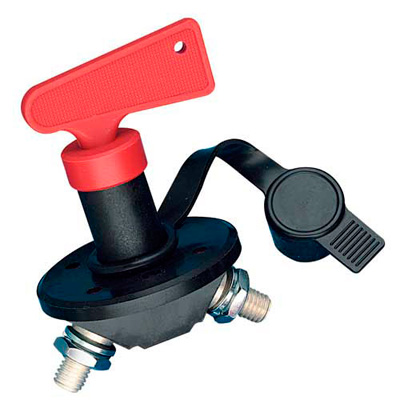
\includegraphics[width=.5\textwidth]{./img/SDC-TSMS.jpg}
	\caption{TSMS.}
	\label{fig:SDC-TSMS}
\end{figure}

\paragraph{Shutdown Switch}
We use OMRON A165E shutdown buttons, which have 3A current rating at 30VDC.

On the cockpit it is OMRON A165E-LS, shown on \ref{fig:SDC-A165E-LS}.
\begin{figure}[H]
	\centering
	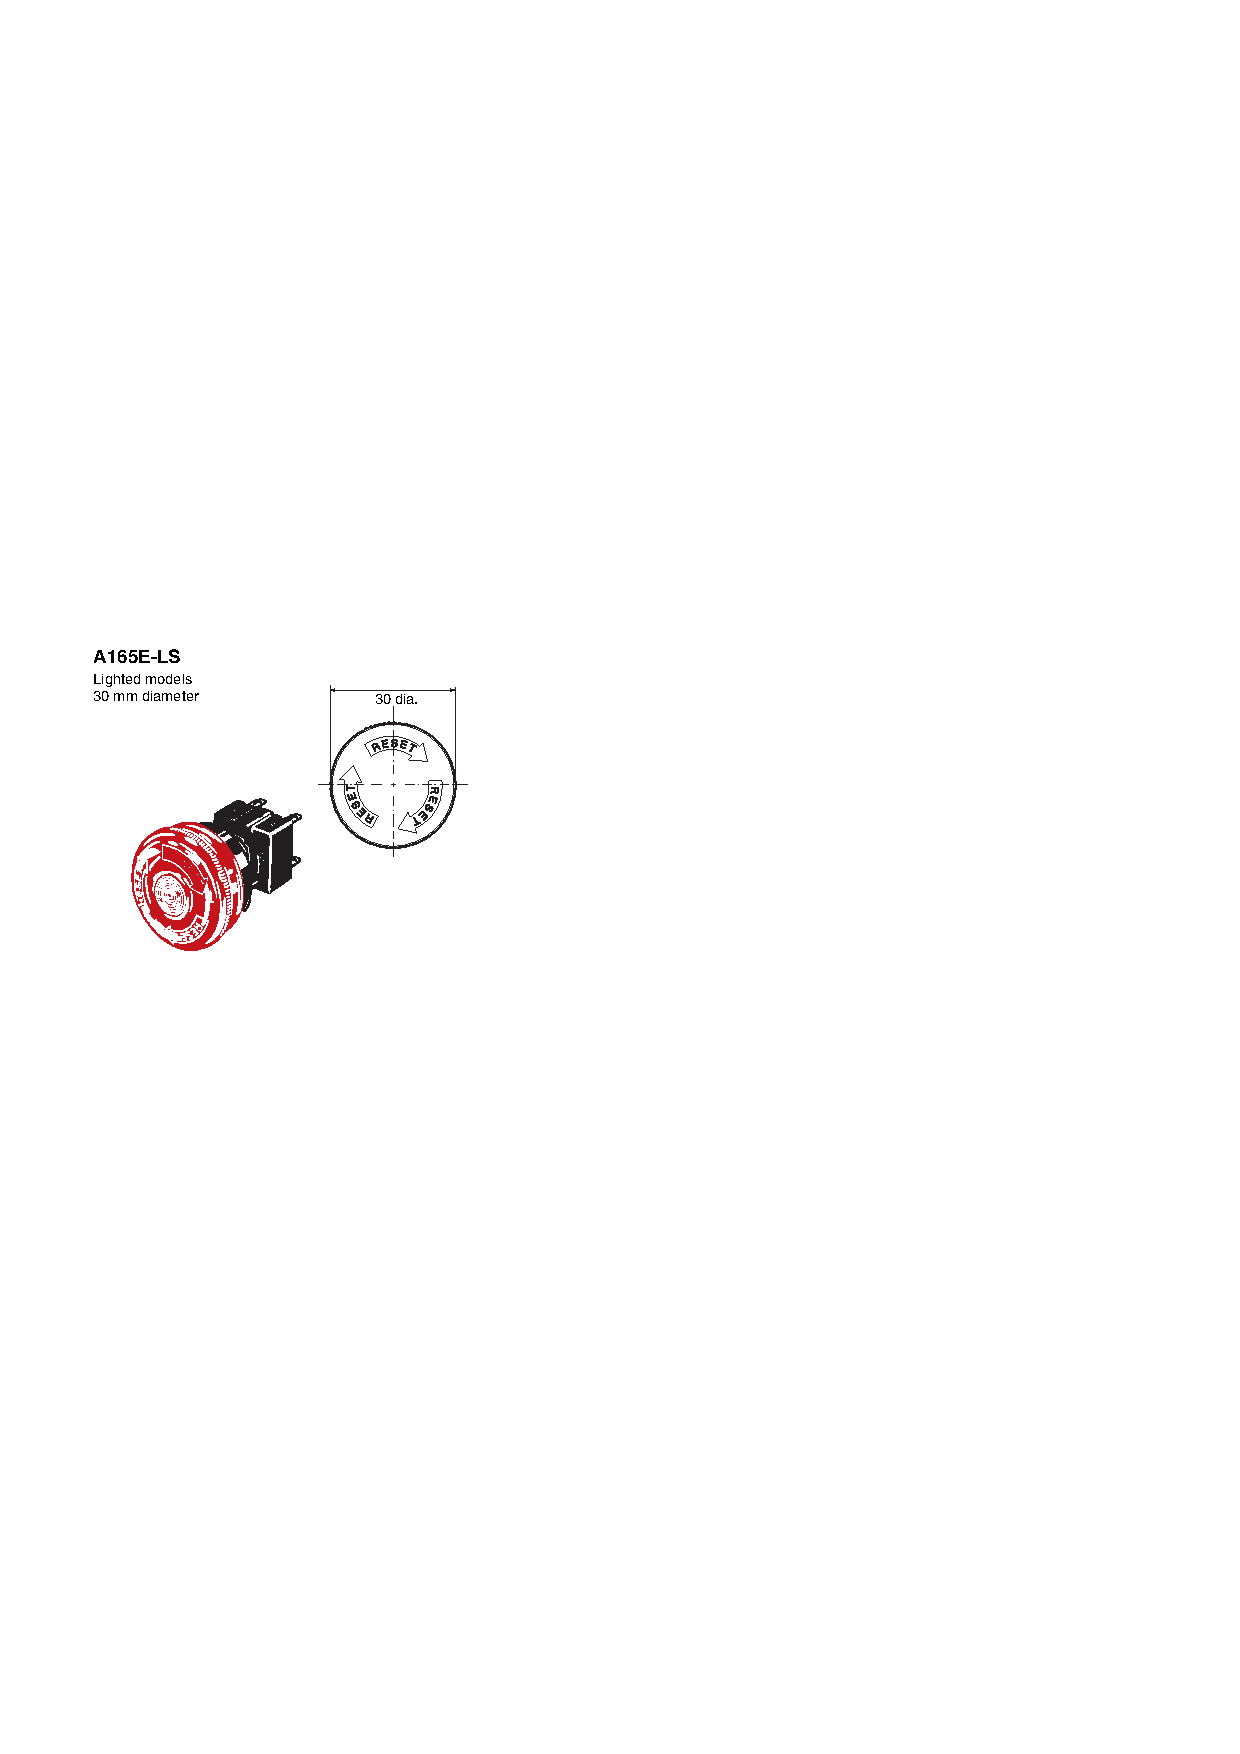
\includegraphics[width=.5\textwidth]{./img/SDC-A165E-LS.pdf}
	\caption{Cockpit SDB.}
	\label{fig:SDC-A165E-LS}
\end{figure}

On the left and on the right sides there are OMRON A165E-LM buttons, shown on \ref{fig:SDC-A165E-LM}.
\begin{figure}[H]
	\centering
	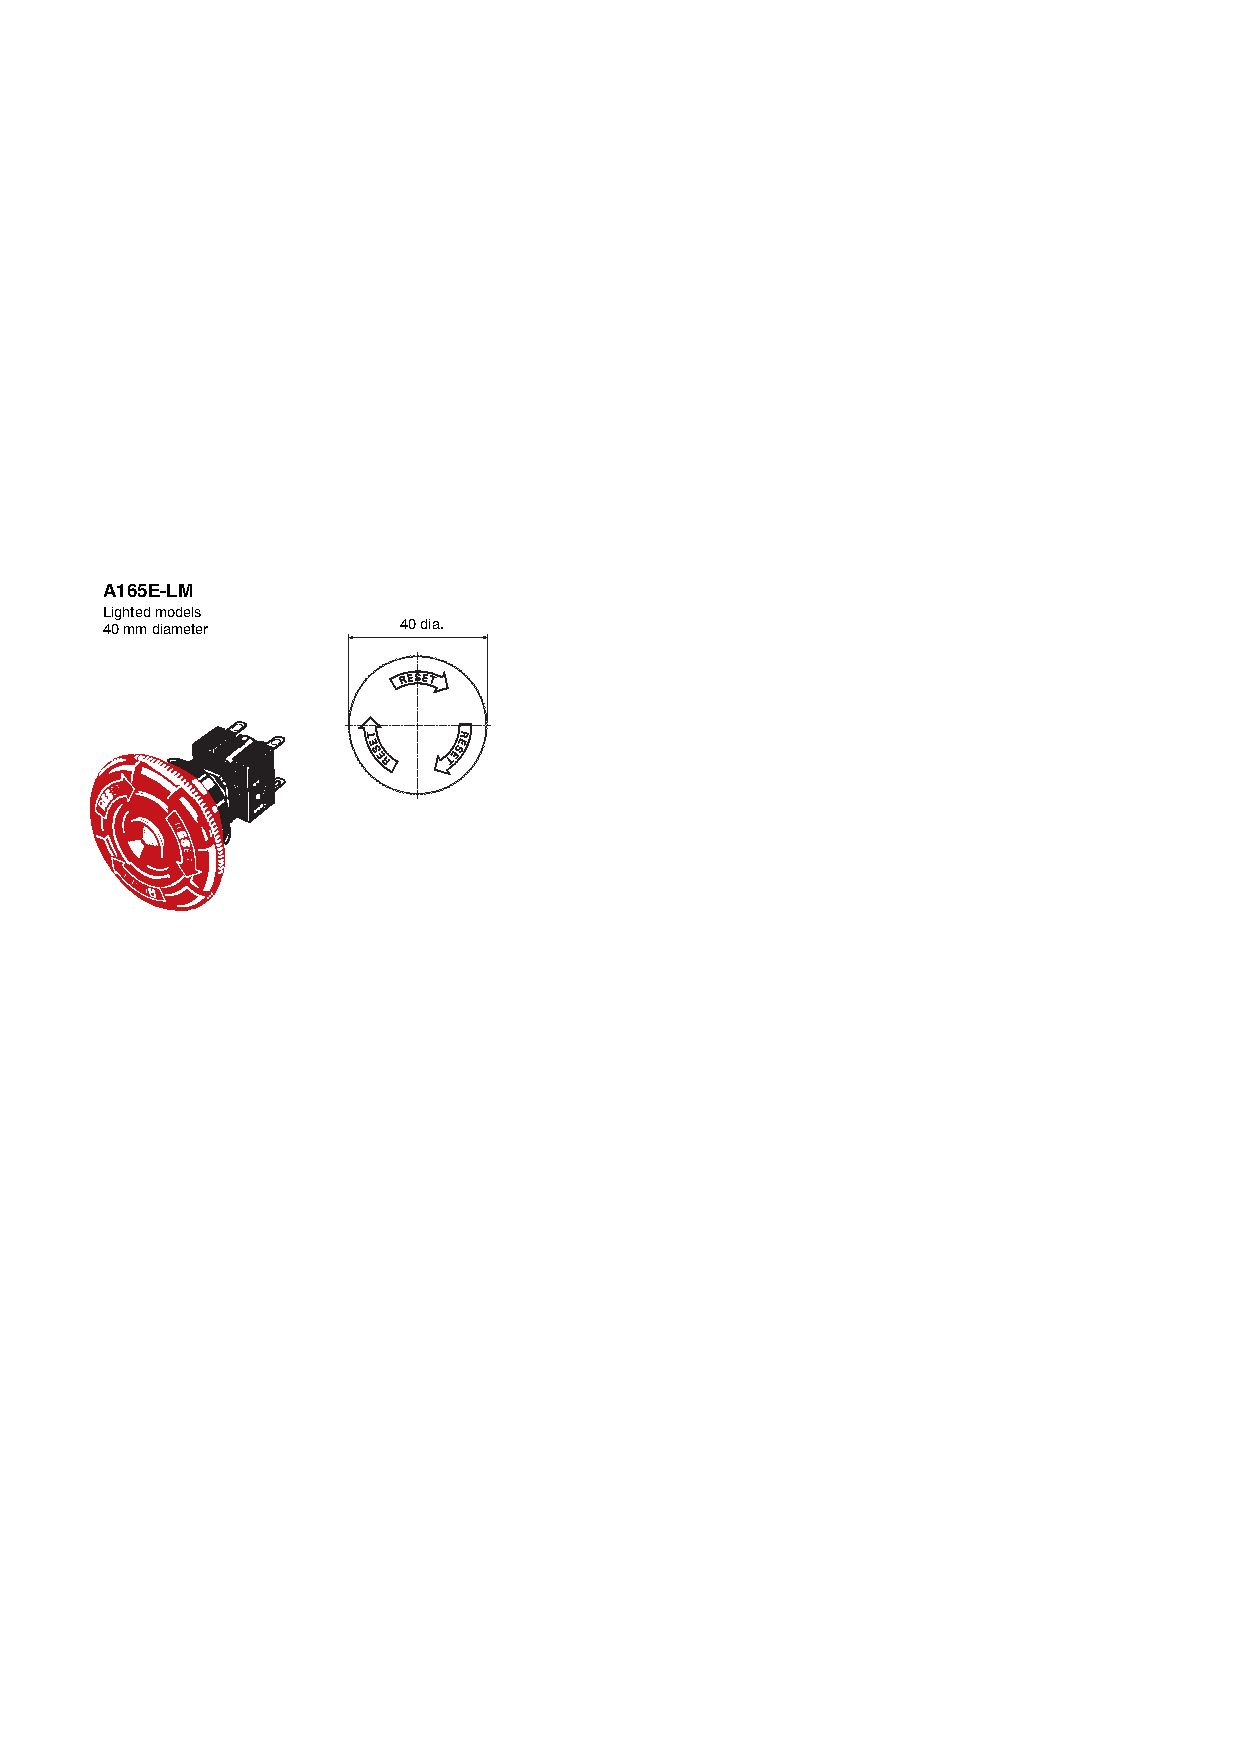
\includegraphics[width=.5\textwidth]{./img/SDC-A165E-LM.pdf}
	\caption{SDB left and right.}
	\label{fig:SDC-A165E-LM}
\end{figure}

\paragraph{Brake Over Travel Switch}
It is type A165E-M, current raging 3A, shown on \ref{fig:SDC-A165E-M}
\begin{figure}[H]
	\centering
	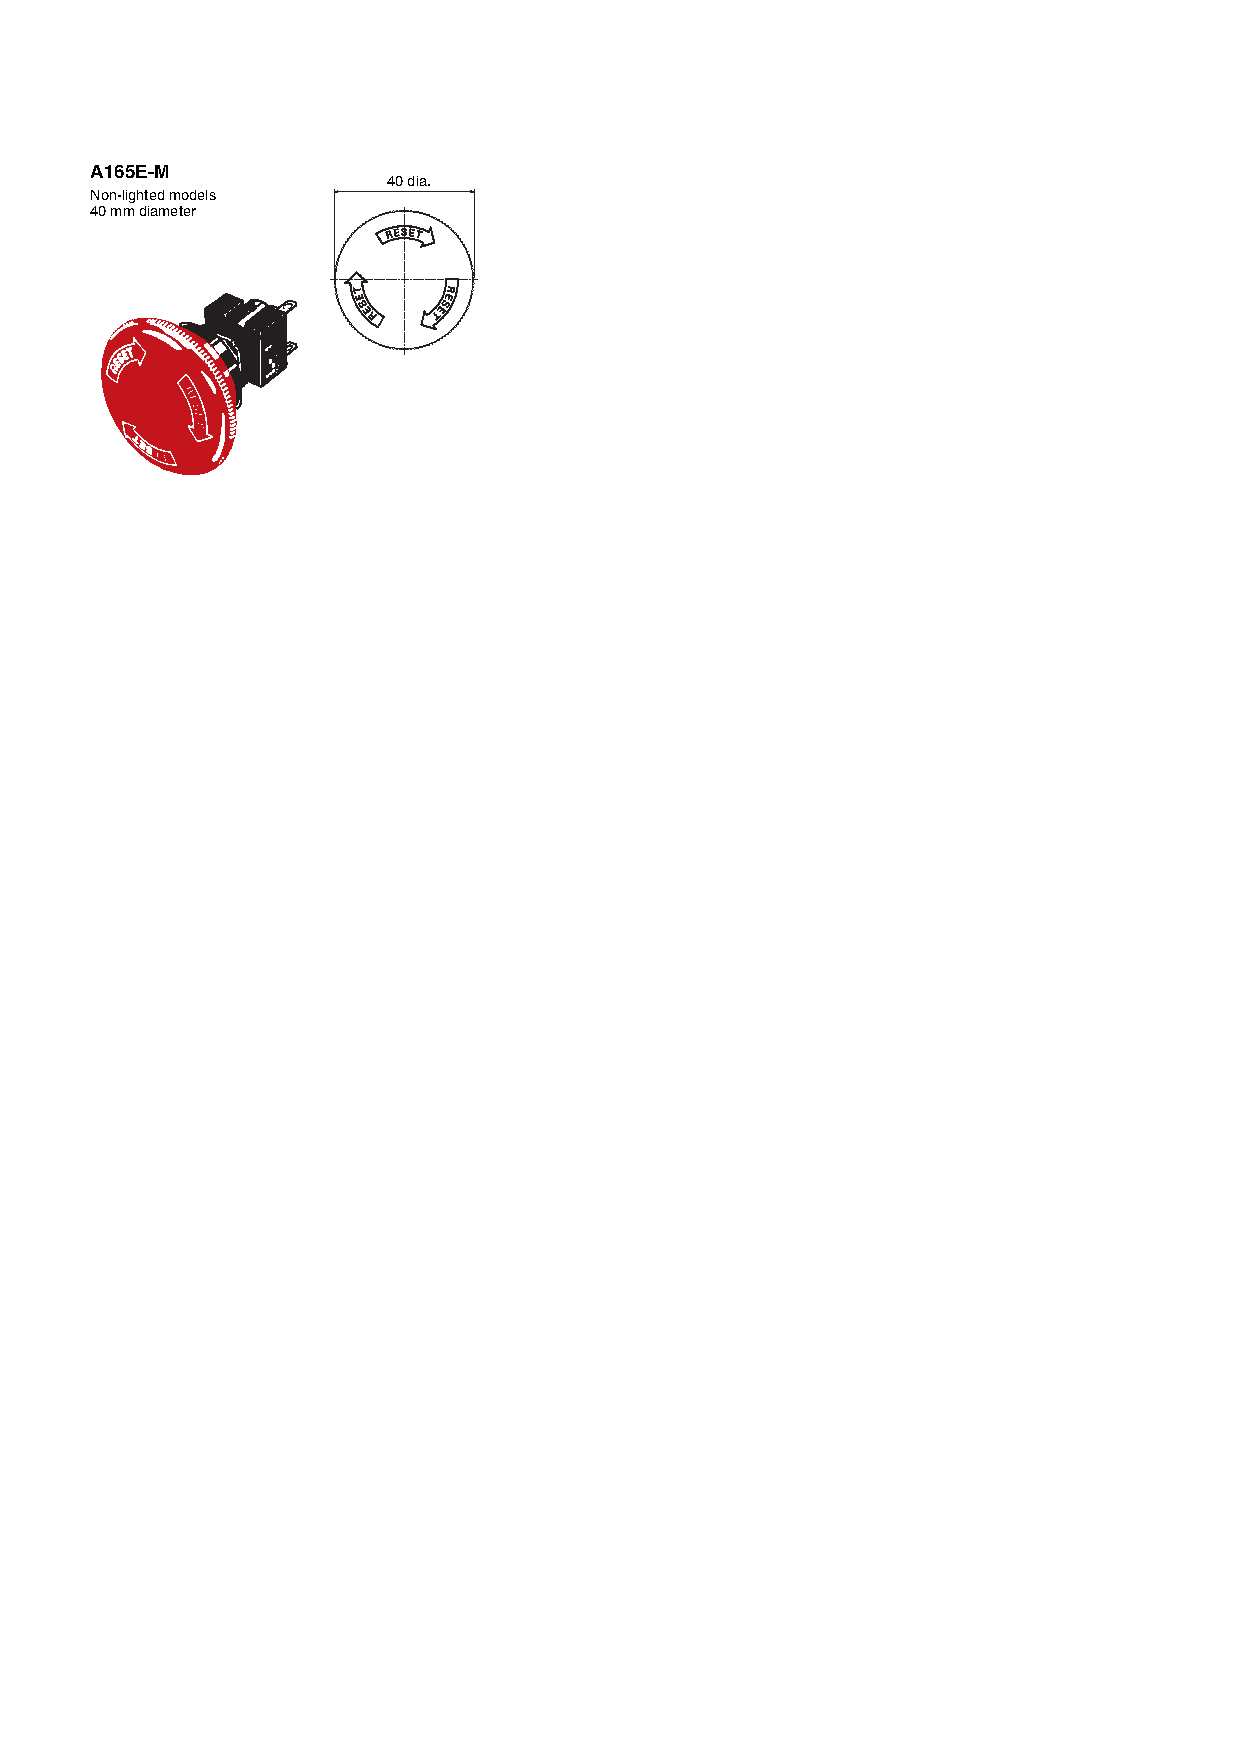
\includegraphics[width=.5\textwidth]{./img/SDC-A165E-M.pdf}
	\caption{Brake over travel switch.}
	\label{fig:SDC-A165E-M}
\end{figure}


\subsubsection{Wiring / additional circuitry}
\iffalse
Describe wiring and additional circuitry, show extra schematics for example if additional transistors etc. are used, also describe the function of additional circuitry and make good use of figures.
Additionally, fill out and add information to the following table:
\fi

If connector is used to connect SDC between control units, disconnecting any of them results in opening SDC and therefore opening AIRs as well. In other words the SDC directly carries the current driving the accumulator isolation relays(AIRs). All circuits that are part of the shutdown circuit have been designed in a way, that, when in disconnected state, they remove the current controlling the AIRs.

The cross-section of Shutdown System wire is AWG22. Block wiring scheme shown on \ref{fig:SDC-schematic}.\\

\begin{figure}[H]
	\centering
	
\includegraphics[width=\textwidth]{./img/sdc-schematic.jpg}
	\caption{Example of used SDC monitoring method with optocouplers.}
	\label{fig:SDC-schematic}
\end{figure}

As shown, 4k7 resistors are used to limit current through optocoupler. With 24V supply that makes 15,2mA per optocoupler. We used 8 optocouplers => 12*15, 2= 182,4mA.
% Table generated by Excel2LaTeX from sheet 'List1'
\begin{table}[H]
	\centering
	\caption{Wiring – Shutdown circuit}
	\begin{tabularx}{\textwidth}{|X|X|}
		\hline
		Total Number of AIRs: & 2 \\[\TableSize]
		\hline
		Current per AIR: & 70mA \\[\TableSize]
		\hline
		Additional parts consumption within the shutdown circuit: & 182,4mA \\[\TableSize]
		\hline
		Total current: & 322,4mA \\[\TableSize]
		\hline
		Cross sectional area of the wiring used: & 0,322mm2 (AWG22) \\[\TableSize]
		\hline
	\end{tabularx}%
	\label{tab:SDC-Wiring}%
\end{table}%


\subsubsection{Position in car}
\iffalse Provide CAD-renderings showing the relevant parts. Mark the parts in the renderings, if necessary. \fi
\begin{figure}[H]
	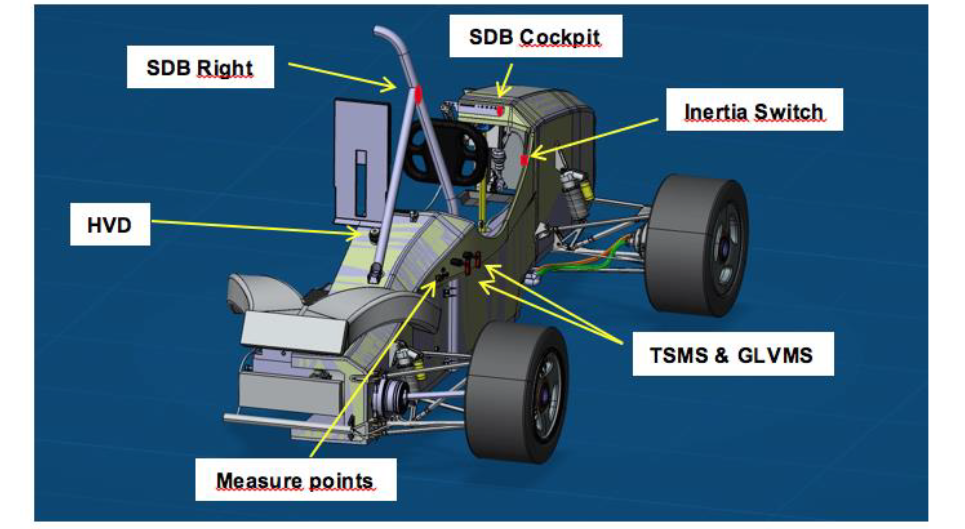
\includegraphics[width=\textwidth]{./img/SDC-positionInCar.png}
	\caption{IMD position.}
	\label{fig:SDC-positionInCar}
\end{figure}

\subsection{IMD}
% chybi tady reference na datasheet
\subsubsection{Description (type, operation parameters)}
\iffalse Describe the IMD used and use a table for the common operation parameters, like supply voltage, set point, etc. Also, describe how the IMD indicator light is wired, etc.
Additionally, fill out the following table replacing the values with your specification:\fi

We use A-ISOMETER® IR155-3203 Insulation monitoring device (IMD) for unearthed DC drive systems. Our maximum tractive voltage is 403.2 VDC. The rules require minimal insulation value between TS and GLVS 500 Ohm/V. Minimal resistance value for our car is 403.2*500 = 201 600 Ohm. This was set as request for manufacturer, and device was programmed in factory.
\begin{table}[H]
	\centering
	\caption{Parameters of the IMD}
	\begin{tabularx}{\textwidth}{|X|l|}
	 \hline	Supply voltage range: & 10..36VDC \\[.4cm]
	 \hline	Supply voltage & 24VDC \\[.4cm]
	 \hline	Environmental temperature range: & -40..105°C \\[.4cm]
	 \hline	Selftest interval: & Always at startup, then every 5 minutes \\[.4cm]
	 \hline	High voltage range: & DC 0..1000V \\[.4cm]
	 \hline	Set response value: & 201.6kΩ (500Ω/Volt) \\[.4cm]
	 \hline	Max. operation current: & 150mA \\[.4cm]
	 \hline	Approximate time to shut down at 50\% of the response value: & 20s \\[.4cm]
	  \hline
	\end{tabularx}%
	\label{tab:IMD}%
\end{table}%

\subsubsection{Wiring/cables/connectors/}
 Describe wiring, show schematics, describe connectors and cables used and show useful data regarding the wiring including wire gauge/temp/voltage rating and fuses protecting the wiring. 

\iffalse Relay of Insulation Monitoring Device is electrically placed between relay in ECUB and relay for AMS measurement. Wiring is done using Raychem Spec44 wire, AWG 26, rated to 600V. Wiring is shown on \ref{label}. Fusing is shown at \ref{label}. IMD opens relay in case of fault. IMD have output for relay, so there is not necessary adding zero diode on output. HV input to IMD is connected in according to datasheet. \fi

\subsubsection{Position in car}
Provide CAD-renderings showing the relevant parts. Mark the parts in the rendering, if necessary

\begin{figure}[H]
	\centering
	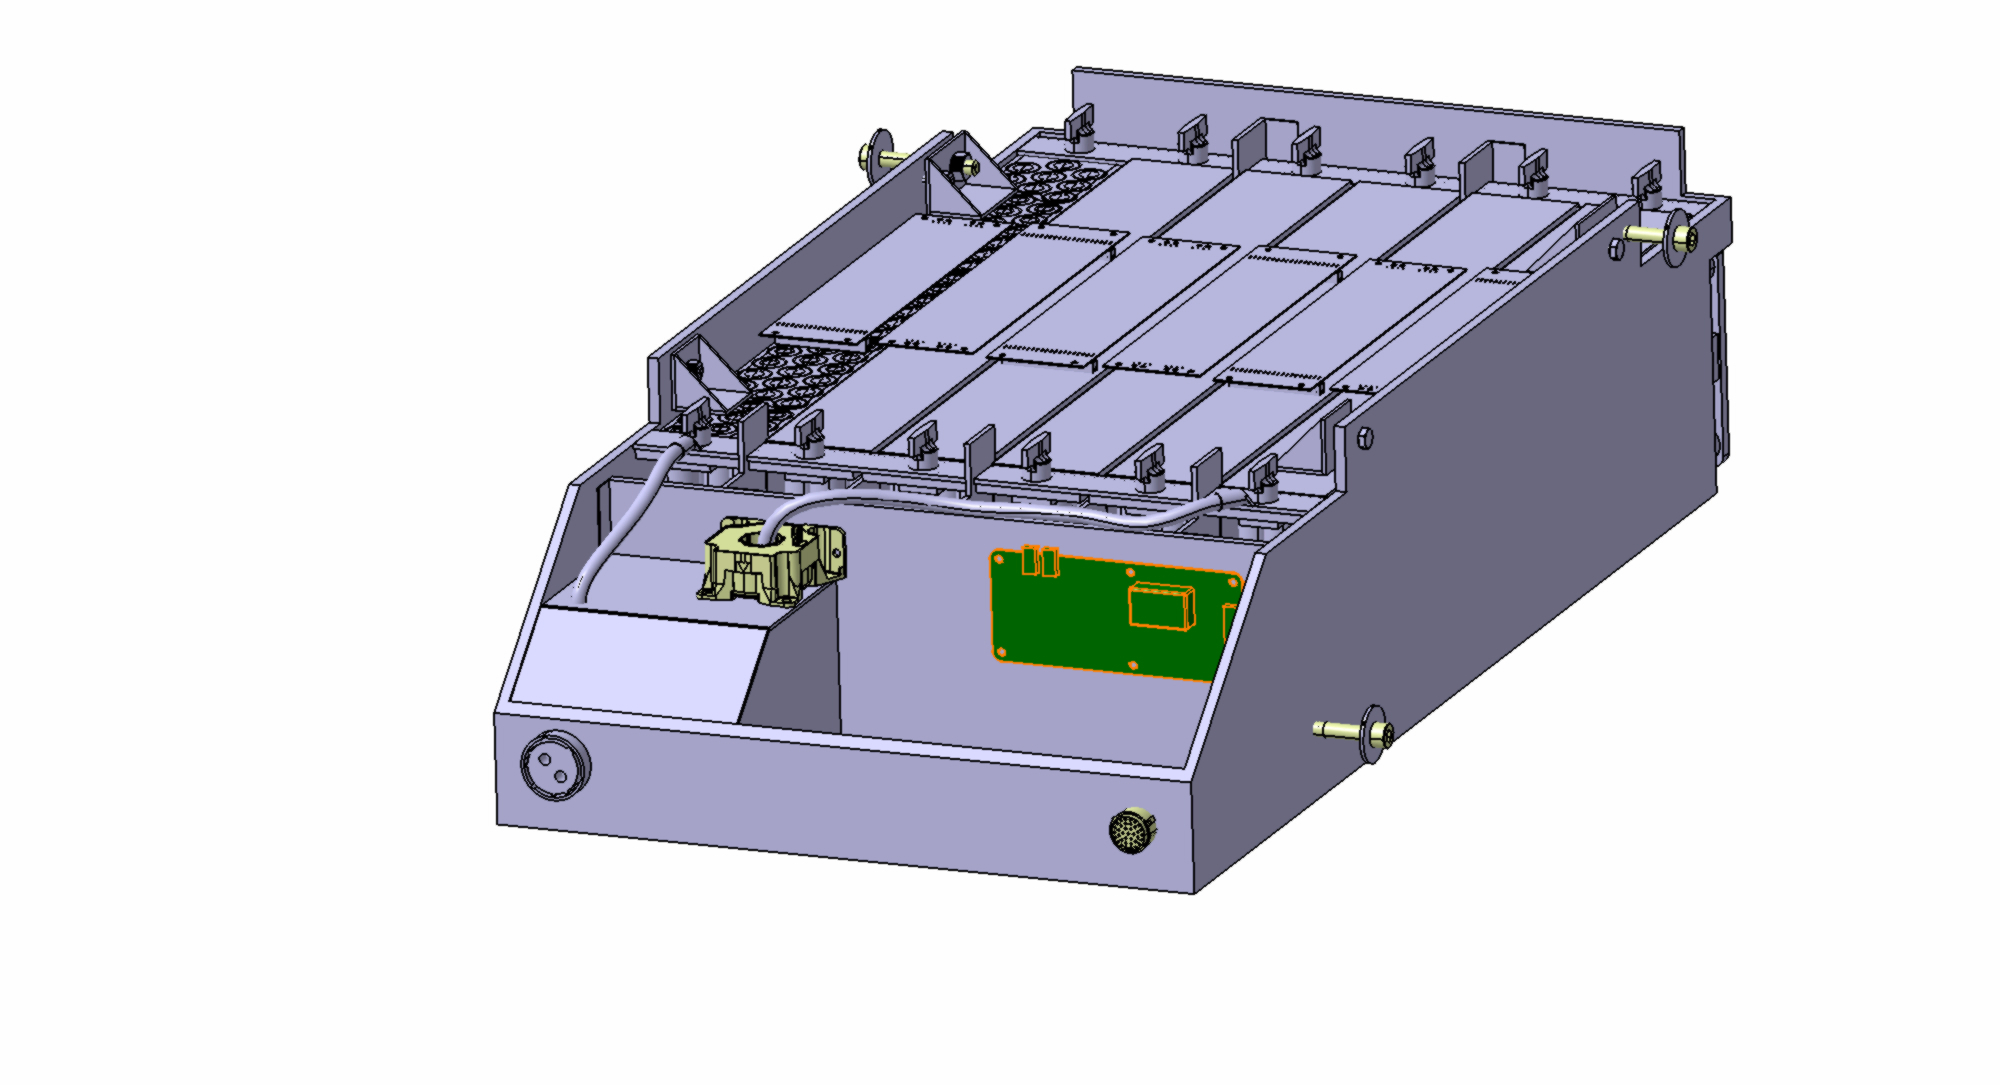
\includegraphics[width=\textwidth]{./img/IMD-position.jpg}
	\caption{IMD position.}
	\label{fig:IMD-position}
\end{figure}
\label{sebsec:IMD}

\subsection{Inertia Switch} \label{subsec:InertiaSwitch}
% nefunguje odakzy
\subsubsection{Description (type, operation parameters)}
\iffalse Describe the Inertia Switch used and use a table for the common operation parameters, like supply voltage, temperature, etc.
Additionally, fill out the following table replacing the values with your specification: \fi

Inertia switch opens shutdown circuit in case of acceleration more than 6g. After acting the driver can reset this switch.
\begin{table}[H]
	\centering
	\caption{Parameters of the Inertia Switch}
	\begin{tabularx}{\textwidth}{|X|l|}
	\hline	Inertia Switch type: & Sensata 510FCS01-01 \\[\TableSize]
	\hline	Supply voltage range: & No supply needed \\[\TableSize]
	\hline	Supply voltage: & No supply needed \\[\TableSize]
	\hline	Environmental temperature range: & -30..120°C \\[\TableSize]
	\hline	Max. operation current: & 10A \\[\TableSize]
	\hline	Trigger characteristics: & 6g for 60ms / 11g for 15ms \\[\TableSize]
	\hline
	\end{tabularx}%
	\label{tab:inertiaSwitch}%
\end{table}%


\subsubsection{Wiring/cables/connectors}
%Describe wiring, show schematics, describe connectors and cables used and show useful data regarding the wiring.

Inertia switch is electrically placed between Shutdown button center on dashboard and the Shutdown input to ECUB, where is connected right Shutdown button on main hoop. Inertia switch will be connected by FQCT connectors. Wiring of inertia switch is shown on \ref{fig:SDC-scheme}. Wiring of inertia switch is shown on \ref{fig:sdc-schema}.
\subsubsection{Position in car}
%Provide CAD-renderings showing the relevant parts. Mark the parts in the rendering, if necessary.

Inertia switch is placed on the right side in the cockpit clearly shown in \ref{fig:SDC-positionInCar}.

\subsection{Brake Plausability Device} \label{subsec:BSPD}
% Responsible: Mark G.
% Author: Mark G.

\subsubsection{Description/additional circuitry}
% Describe how your electronic hardware brake plausibility system works (this is in addition to your ECU controlled brake plausibility software), provide tables with main operation parameters, and describe additional circuitry used to check or for an implausibility. Describe how the system reacts if an implausibility or error is detected.

BSPD is represented by a PCB with an on-board current transducer. Brake state signal is received via wiring from ECUP. Output controls Gate of a MOSFET, that acts as a “normally-closed” switch in SDC loop. In case of a trip event output changes state and gets latched till a GLVMS restart.

\begin{table}[H]
	\centering
	\caption{BSPD data}
	\begin{tabularx}{\textwidth}{|X|X|}
		\hline
		Brake sensor used: & Piezoresistive Pressure Transmitter PA-21Y / 100bar / 81691.1 \\[\TableSize]
		\hline
		Brake sensor physical response value: & Voltage, 4,5V \\[\TableSize]
		\hline
		Tractive system power sensor type & Current Transducer LEM HTFS 200-P \\[\TableSize]
		\hline
		Tractive system sensor physical response value: & Voltage of 85mV \\[\TableSize]
		\hline
		Tractive System power sensor current treshold (5kW/Nominal TS voltage): & 14A \\[\TableSize]
		\hline
		Supply voltages: & 5V \\[\TableSize]
		\hline
		Maximum supply currents: & 22mA \\[\TableSize]
		\hline
		Operating temperature: & -40..105$\circ$C\\[\TableSize]
		\hline
		Output used to control AIRs: & Open a MOSFET in SDC \\[\TableSize]
		\hline
	\end{tabularx}%
	\label{tab:addlabel}%
\end{table}%

\begin{figure}[H]
	\centering
	
\includegraphics[width=\textwidth]{./img/bspd-position.jpg}
	\caption{BSPD flowchart.}
	\label{fig:BSPD-flowchart}
\end{figure}

\subsubsection{Schematic}
Describe the wiring, show schematics including the circuit board, show data regarding the cables and connectors used

\begin{figure}[H]
	\centering
	
\includegraphics[width=\textwidth]{./img/bspd-position.jpg}
	\caption{Connection with the SDC schematic.}
	\label{fig:BSPD-conn}
\end{figure}

\subsubsection{Connection with shutdown circuit}

\begin{figure}[H]
	\centering
	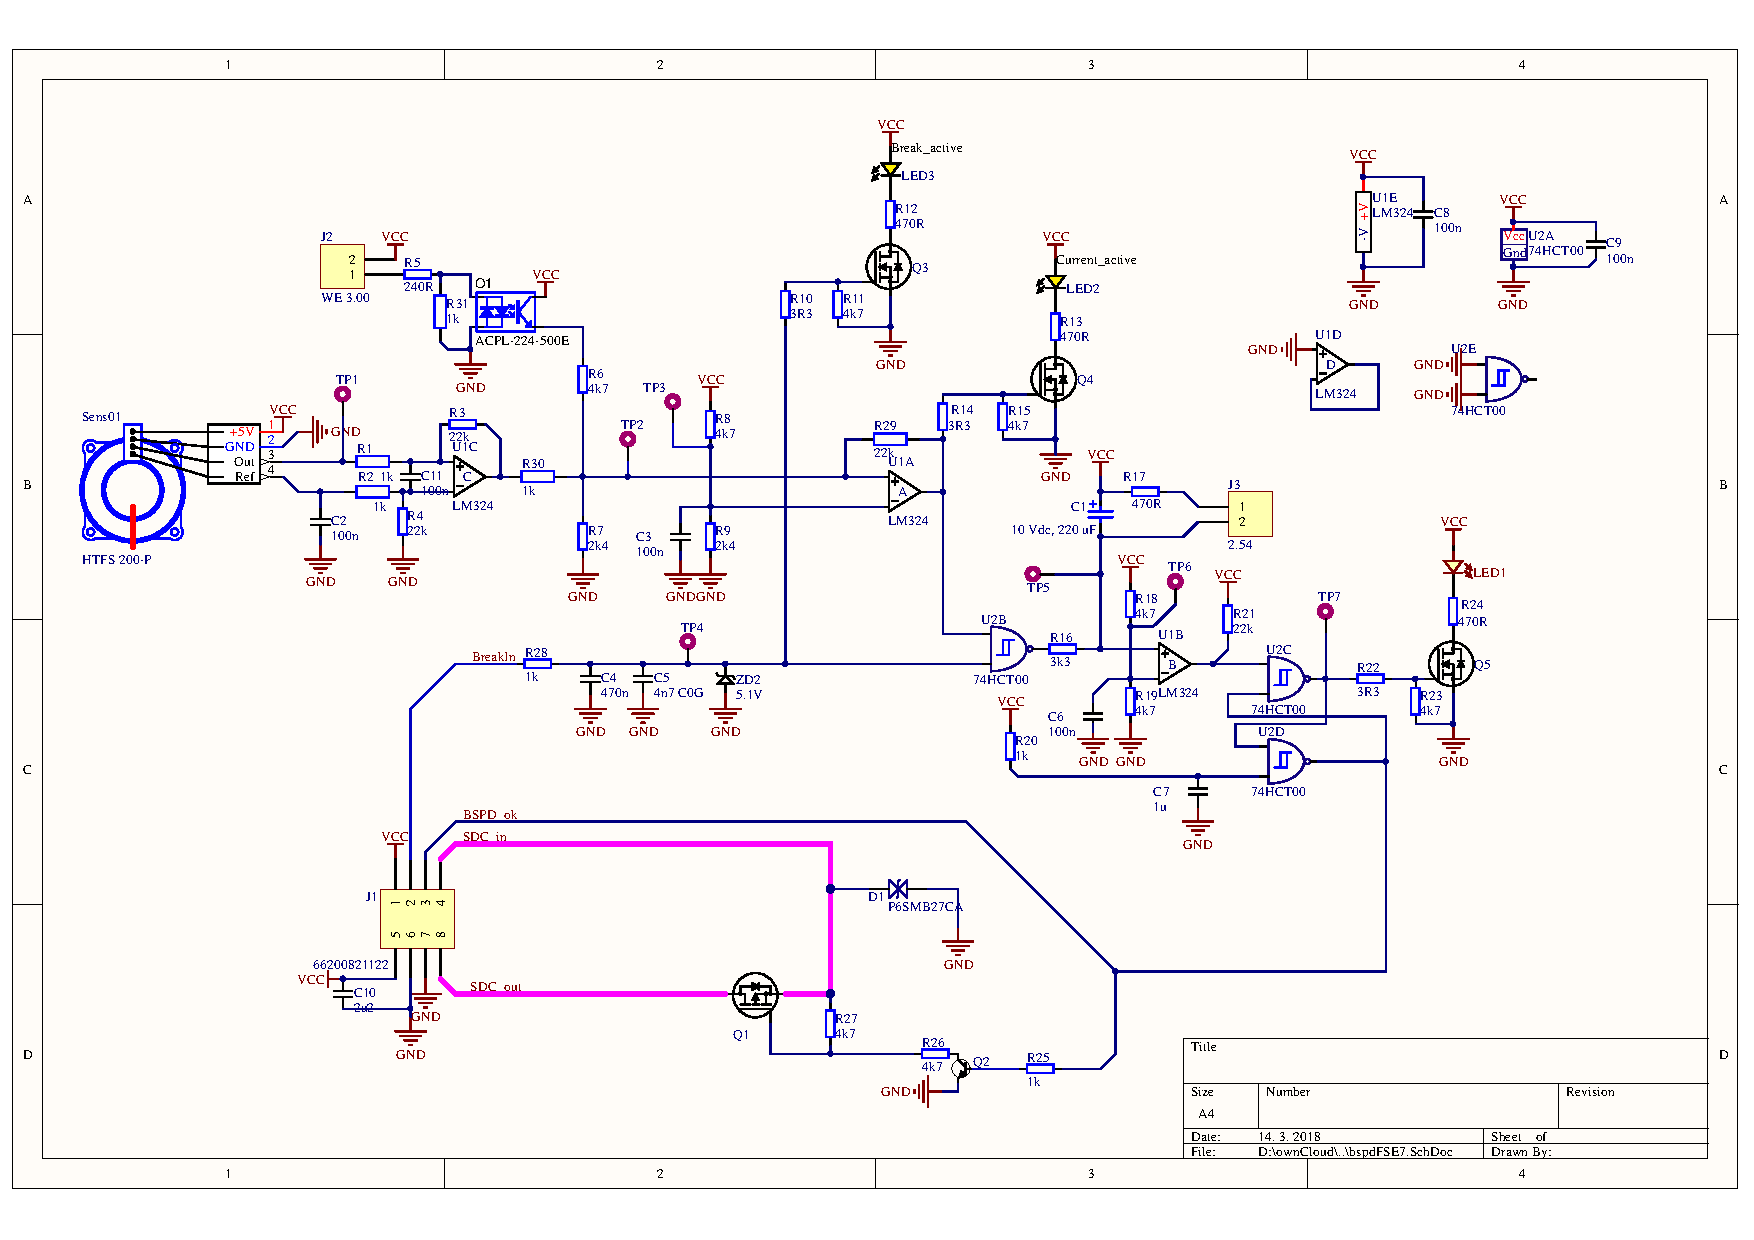
\includegraphics[width=\textwidth]{./img/bspd-schematic.pdf}
	\caption{BSPD schematic sheet.}
	\label{fig:BSPD-schematic}
\end{figure}

\subsubsection{Position in car/mechanical fastening/mechanical connection}
Provide CAD-renderings showing all relevant parts and discuss the mechanical connection of the sensors to the pedal assembly. Mark the parts in the rendering, if necessary.

\begin{figure}[H]
	\centering
	
\includegraphics[width=.5\textwidth]{./img/bspd-position.jpg}
	\caption{BSPD position}
	\label{fig:BSPD-position}
\end{figure}


\subsection{Reset / Latching for IMD and BMS} \label{subsec:Reset}
% Responsible: Kdokoliv
% ECUB scheme and circuitry, state machine and other
\subsubsection{Description/circuitry}
% Describe the concept and circuitry of the latching/reset system for a tripped IMD or AMS.  Describe the method for resetting the IMD and AMS.

\subsubsection{Wiring/cables/connectors}
\iffalse Describe wiring, show schematics, describe connectors and cables used and show useful data regarding the wiring.  If not detailed in section 2.1, be sure to show how the device opens the shutdown circuit.\fi
% SDC monitoring scheme 
Measuring, what was original problem, is done by two optocouplers in ECUB. Figure 16 - Example of used SDC monitoring with optocouplers.
\subsubsection{Position in car}
%Provide CAD-renderings showing the relevant parts. Mark the parts in the rendering, if necessary.
Latch as well as reset of IMD and BMS error is placed in ECUB box on the back of car. See \ref{fig:sdc-position}.

\subsection{Shutdown System Interlocks}\label{subsec:SDCInterlocks}
% figures and renderings 
%Responsible: Jano
\subsubsection{Description/circuitry}
\iffalse Describe the concept and circuitry of the Shutdown System Interlocks.
Note: Interlocks are circuits used to open the shutdown circuit if a connector is disconnected or enclosure is opened.  This is not the entire shutdown circuit.\fi

We have interlocks in ACP HV connector (connector HV\_A), Motor controller HV inputs and outputs, HV connector in Service box, HVD and in the LV connectors from ECUM´s (ECUM Rear and ECUM Front) to motor (connectors M1, M2, M3 and M4). In the M1-4 connectors we have a loop, that protects motor from disconnecting from a vehicle (disconnection of any of them triggers the Shutdown circuit).

\subsubsection{Wiring/cables/connectors}
%Describe wiring, show schematics, describe connectors and cables used and show useful data regarding the wiring.

Scheme of entire Shutdown circuit can be found at Figure 6 - Block SDC wiring scheme
\subsubsection{Position in car}
%Provide CAD-renderings showing the relevant parts. Mark the parts in the rendering, if necessary.
HVD is clearly shown above in Figure 8 - Inertia switch, SDB Left, Right and Cockpit, TSMS, GLVMS, HVD, Measure points. For Service box position see Figure 17 - Motor controllers

Last interlock is in Accumulator Pack HV Connector shown in ACP HV Connector.

\subsection{Tractive System Active Light}\label{subsec:TSAL}
% Responsible: Janko, Emil, Manek
%ECUB, schemata tsal + schema v ecub + schemes + renders
\subsubsection{Description / circuitry}
% Describe the tractive system active light and additional circuitry. Additionally, fill out the table:

Our TSAL system is consists of two parts, LEDs and generator of frequency with power-switch. Generator is in ECUB protected by fuse. The waveform is generated with a 555-based circuit. The TSAL uses pairs of anti-parallel LEDs and is connected with two wires. Color of the light is decided by the polarity of the driving voltage. The following table shows the operation mode depending on conditions C1, C2:

% dodat tabulku

EV4.12.1 is achived by U4 in Figure 21 - TSAL HV part schematic comparing the voltage on R59 with 3v3 reference. MHVout is connected to output connector of accumulator. O4 carries the information about HV presence to LV system and enables powerto TSAL by opening Q5.

\begin{figure}[H]
	\centering
	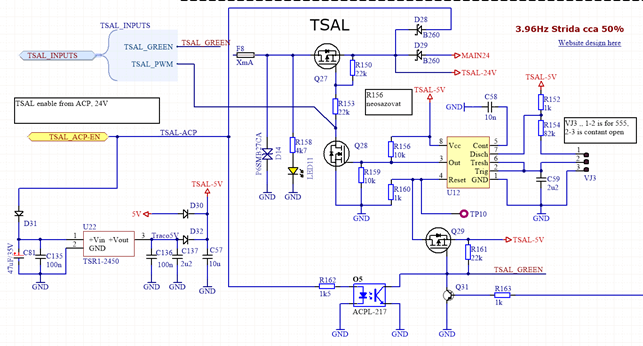
\includegraphics[width=\textwidth]{./img/TSAL-ECUB-schematic.png}
	\caption{Schematic of generator for TSAL.}
	\label{fig:TSAL-ECUB-schematic}
\end{figure}

\begin{table}[H]
	\centering
	\caption{Parameters of the TSAL}
	\begin{tabularx}{\textwidth}{|X|X|}
		\hline
		Supply voltage: & +/- 24VDC \\[\TableSize]
		\hline
		Max. operational current: & 300mA \\[\TableSize]
		\hline
		Lamp type & Bi-color LED \\[\TableSize]
		\hline
		Power consumption: & 7.2 W \\[\TableSize]
		\hline
		Brightness & 124 Lumen (red), 29 Lumen (green) \\[\TableSize]
		\hline
		Frequency: & 3.96Hz \\[\TableSize]
		\hline
		Size (length x height x width): & 128mm x 20mm x 32mm \\[\TableSize]
		\hline
	\end{tabularx}%
	\label{tab:TSAL}%
\end{table}%

\begin{figure}[H]
	\centering
	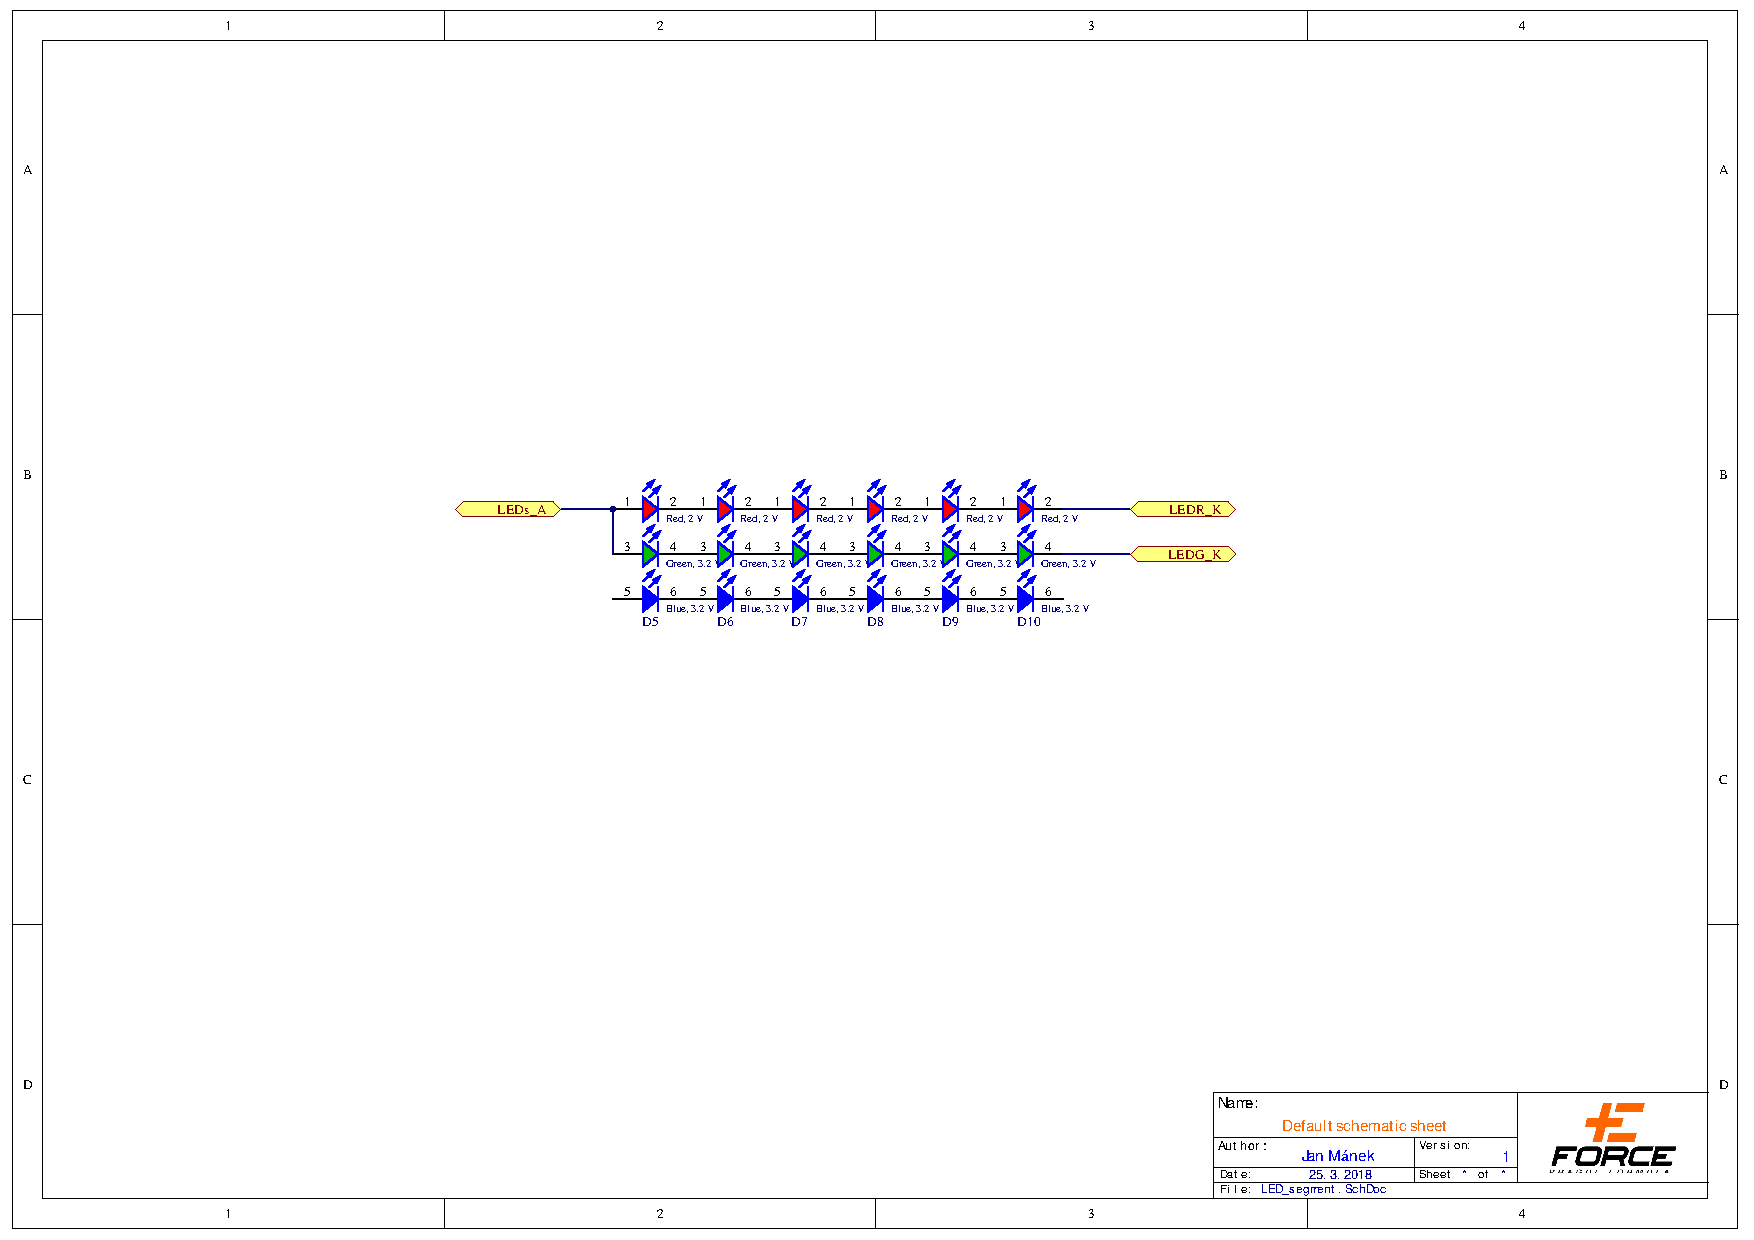
\includegraphics[width=\textwidth,trim={6cm 10cm 6cm 7cm},clip]{./img/TSAL-schematic.pdf}
	\caption{TSAL schematic.}
	\label{fig:TSAL-schematic}
\end{figure}

\begin{figure}[H]
	\centering
	
\includegraphics[width=\textwidth]{./img/tsal-wiring.jpg}
	\caption{TSAL HV part schematic.}
	\label{fig:TSAL-HV}
\end{figure}

\paragraph{Explanation of TSAL circuit}

Left top corner of \ref{fig:TSAL-HV} (input marked as HV-Viper) is directly connected to the output HV pins of ACP. The circuit is designed with STM chip „VIPER16HN“. It behaves as normal fly-back, with input voltage range from 50V up to 500V. Output of flyback is used to directly power the TSAL. ACP indication led is powered from primary side of transformer. To ensure corect beahviour we also measure and comapre input voltage (using U12A OAMP as comparator with little hysteresis), to enable output (Q36 \& Q33) only if input voltage is >=60VDC.

\begin{figure}[H]
	\centering
	
\includegraphics[width=\textwidth]{./img/tsal-wiring.jpg}
	\caption{TSAL enable scheme}
	\label{fig:TSAL-enable}
\end{figure}

Function of circuit on \ref{fig:TSAL-enable} is that the TSAL is enabled even when the 60VDC limit is not reached but the AIR is closed nonetherless. In such state, the TSAL is enabled by signal AIR\_EN. The circuit is powered by MAIN24 power (which is equal to the 24V enabled by GLVMS) or by the TSAL\_ACP-EN power signal from the Viper-TSAL schematic (\ref{fig:TSAL-ACPindicator}) below.

\begin{figure}[H]
	\centering
	
\includegraphics[width=\textwidth]{./img/tsal-wiring.jpg}
	\caption{ACP indication LED wiring}
	\label{fig:TSAL-ACPindicator}
\end{figure}

%schema z backu
\subsubsection{Wiring/cables/connectors}
\iffalse Describe wiring, show schematics, describe connectors and cables used and show useful data regarding the wiring.  Include gauge, voltage and temperature rating of wiring used and any fuses or other overcurrent protection used.\fi

LEDs are supplied from ECUB (by Harness\_D by connector D1) by 2-wire low voltage cable (\ref{fig:TSAL-wiring}).

\begin{figure}[H]
	\centering
	
\includegraphics[width=\textwidth,]{./img/tsal-wiring.jpg}
	\caption{Wiring TSAL from ECUB}
	\label{fig:TSAL-wiring}
\end{figure}

\subsubsection{Position in car}
%Provide CAD-renderings showing the relevant parts. Mark the parts in the rendering, if necessary.
TSAL is placed under the main roll hoop, see \ref{fig:TSAL-position}

\begin{figure}[H]
	\centering
	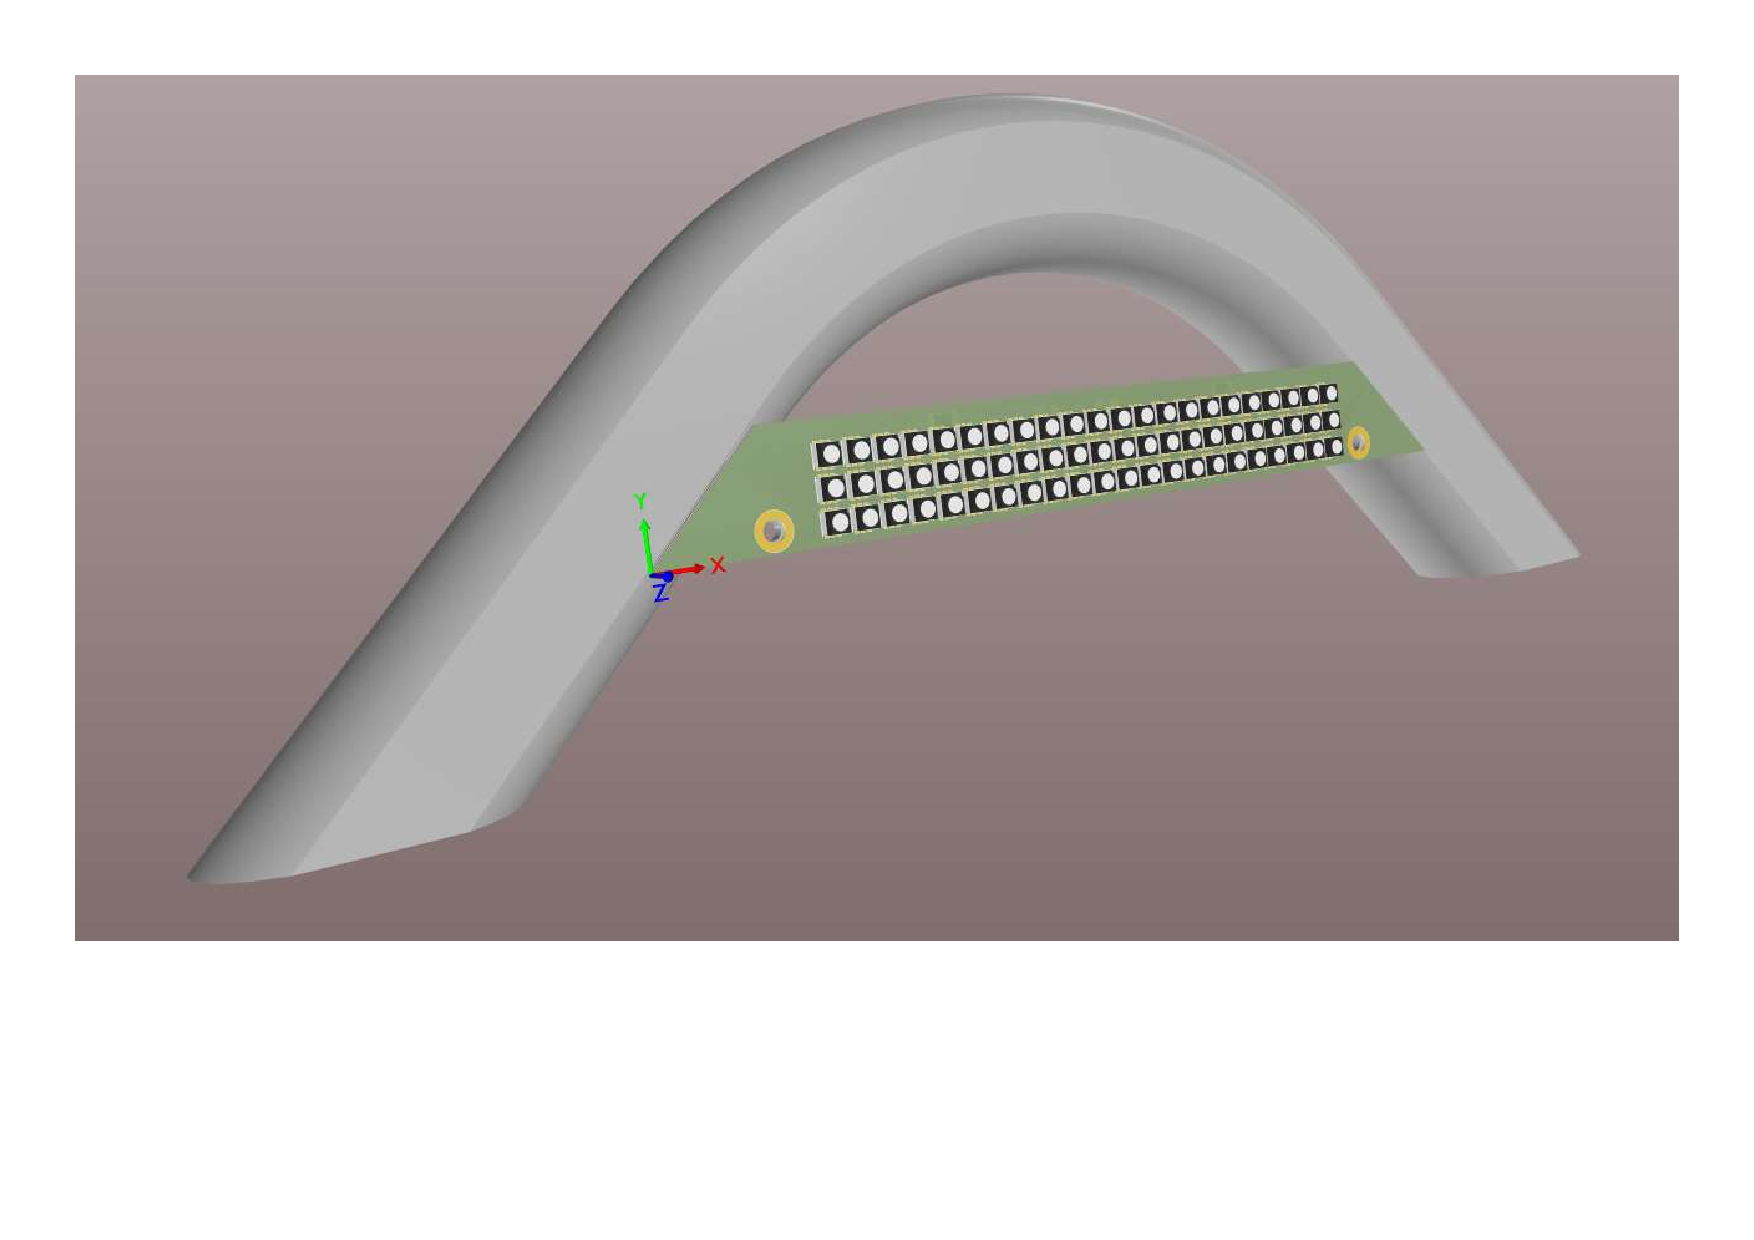
\includegraphics[width=\textwidth,trim={3cm 11cm 2cm 1cm},clip]{./img/tsal-position.pdf}
	\caption{TSAL position.}
	\label{fig:TSAL-position}
\end{figure}

\subsection{Measurement points}\label{subsec:MeasurementPoints}
%Responsible: Janko
%schemata
\subsubsection{Description}
%Describe the housing used and how it can be accessed, etc.  Describe how the measurement points protected/covered when not in use and how the electrical connections on the back of the measurement points are protected when the measurement points are being used.

High voltage measurement points (HVMP) are placed in the Service box. When not in use, they are covered with protective cups made from silicone rubber. From backside they are protected by sealed Service box all the time.
\subsubsection{Wiring, connectors, cables}
%Describe wiring, show schematics, and describe connectors and cables used and show useful data regarding the wiring.  Include details on the protection resistor including resistance, voltage and power rating.

They are connected to ECUB (by Harness\_G with connector G1). In ECUB is TSAL switch circuit and discharge circuit is in ECUM (ECUM is connected to ECUB by Harness\_E – connectors are E1 from ECUB and E2 into ECUM Rear).
HVMP wires will be connected to the board in ECUB box, where is TSAL switch circuit, discharge circuit and 2 resistors 15k 1W (R1, R2) for HVMP. Value of this resistor can be measured from measuring points by multimeter with switched TSMS off.

\subsubsection{Position in car}
%Provide CAD-renderings showing the relevant parts. Mark the parts in the rendering, if necessary.

Measure points are placed on panel next to Master switches and HVD, see Figure 8 - Inertia switch, SDB Left, Right and Cockpit, TSMS, GLVMS, HVD, Measure points.

\subsection{Pre-Charge circuitry}\label{subsec:PrechargeCircuitry}
%Responsible: JSi
%ECUA
\subsubsection{Description}
%Describe your concept of the pre-charge circuitry.
Pre-charge circuit is controlled by ECUA. (Isolation on PCB is refered from 8.3Electronic control unit acp (ECUA)) Our pre-charge is assembled from 3 resistors. 2 of them have the same value 470R, the third is mainly part of safety precaution and has value 2k2. There is always a chance that the resistor fails, in that case the remaining resistors may be used as fully functional pre-charge, only slower.

TS ON button sets whole car in state ‘pre-charging’. ECUA starts pre-charge process. It takes safety precautions and then relay and AIR are switched to close pre-charging current. Fully closed SDC and ECUA decision are needed to start pre-charging. If every point is fulfilled and pre-charge is successfully finished, second AIR closes. Pre-charge relay opens and car leaves pre-charge state. (Pre-charge relay is normally open type.)
% chybi schema - Honza doplni

\paragraph{Pre-charge safety on ECUA}
Except from what rules require we implemented several safety precautions. In case, that SDC error doesn’t occur and driver pushed TS ON button following safety precautions are taken to prevent switching AIR in case of problem that has not yet been detected.

First one is completely non-programmable protection against switching voltage difference by AIR. It uses voltage measurement and then comparators and logic to disable microcontroller decision in case of SW error.
Second one is measuring all states and voltages by microcontroller on ECUA which can determinate error before non-programmable protection would have to act.

Third (time-out) protection is used when everything seems to be OK, but the charging is too slow – caused by too high pre-charge resistance (any of pre-charge resistors fails), or some leakage of charge in capacitor or any other possible error occurs. If voltage difference is not equaled in time less them 2seconds, the ECUA stops pre-charge and waits 5 seconds before trying again. (In order to not overpower resistors.) If number of attempts to pre-charge is in this state higher then 8, something is clearly wrong and ECUA opens SDC and indicates error. Sending message about error and sets car into not-ready state.

\subsubsection{Wiring, cables, current calculations, connectors}
Describe wiring, show schematics, describe connectors and cables used and show useful data regarding the wiring.
\begin{itemize}
\item Give a plot “Percentage of Maximum Voltage” vs. time
\item Give a plot Current vs. time 
\item For each plot, give the basic formula describing the plots
\end{itemize}

Additionally, fill out the tables:

\begin{table}[H]
	\centering
	\caption{General data of the pre-charge resistor}
	\begin{tabularx}{\textwidth}{|X|X|}
		\hline
		Resistor Type: & \\[\TableSize]
		\hline
		Resistance: & \\[\TableSize]
		\hline
		Continuous power rating: & \\[\TableSize]
		\hline
		Overload power rating (1 sec): &  \\[\TableSize]
		\hline
		Overload power rating (5 sec): &  \\[\TableSize]
		\hline
		Overload power rating (15 sec): &  \\[\TableSize]
		\hline
		Voltage rating: & \\[\TableSize]
		\hline
		Cross-sectional area of the wire used: & \\[\TableSize]
		\hline
	\end{tabularx}%
	\label{tab:precharge-general}%
\end{table}%

\begin{table}[H]
	\centering
	\caption{General data of the pre-charge relay}
	\begin{tabularx}{\textwidth}{|X|X|}
		\hline
		Relay Type: & \\[\TableSize]
		\hline
		Contact arrangment: &  \\[\TableSize]
		\hline
		Continuous DC current:  & \\[\TableSize]
		\hline
		Voltage rating  & \\[\TableSize]
		\hline
		Nominal Coil Voltage: &  \\[\TableSize]
		\hline
		FET type: &  \\[\TableSize]
		\hline
		Maximum Drain-Source Current: &  \\[\TableSize]
		\hline
		Drain-Source Breakdown Voltage: &  \\[\TableSize]
		\hline
		On Charasteristics Gate Threshold Voltage: & \\[\TableSize]
		\hline
		Cross-sectional area of the wire used: & \\[\TableSize]
		\hline
	\end{tabularx}%
	\label{tab:precharge-relay}%
\end{table}%

\subsubsection{Position in car}
Provide CAD-renderings showing all relevant parts. Mark the parts in the rendering, if necessary.

\subsection{Discharge circuitry}\label{subsec:PrechargeSafety}
%ECUB
\subsubsection{Description}
%Describe your concept of the discharge circuitry.

Discharge circuit is activated whenever SDC is open, this is ensured by ECUB which monitors latching of SDC. The idea of discharging capacity is to have discharge resistors in the device with that capacity – so in both Motor Controllers. So ECUB sends message to Motor Controllers and they close circuit with Discharge resistors banks. When AIRs are closed, ECUB informs Motor Controllers and they open discharge circuits.

\begin{figure}[H]
	\centering
	
\includegraphics[width=\textwidth]{./img/tsal-wiring.jpg}
	\caption{Discharge circuit.}
	\label{fig:discharge-circuit}
\end{figure}

\subsubsection{Wiring, calbes, current calculations, connectors}
\iffalse Describe wiring, show schematics, describe connectors and cables used and show useful data regarding the wiring.
\begin{itemize}
	\item 	Give a plot “Voltage” vs. time
	\item 	Give the formula describing this behavior
	\item 	Give a plot “Discharge current” vs. time
	\item 	Give the formula describing your plot
\end{itemize}\fi

Following \ref{fig:discharge-circuit} shows a siplified connection of a discharge resistors. It is connected the same way, only unnecessary detail parts of the circuit were cover as a „block“. The resistor is placed in MC right next to only capacity that provides a storrage for potencially dangerous charge/energy. If the HV cable is disconnected on either side, the SDC opens due to the interlocks and AIRs open. Because there is no output capacitance in ACP there is no way the power could be on ACP output HV connector.

The capacity of all the capacitors in Motor Controllers is in the sum 2360 uF. For discharging this capacity in less than 5 seconds to voltage under 60V, maximum value is calculated by solving R from the formula

with values:
VC = 60 V
VS = 403.2 V
t = 5 s
C = 1180-6 F
The resulting R = 1000 Ohm. In total 8 discharge resistors are used in configuration 2s4p – so 2s2p in each motor controller. Each resistor is type THS151K5J (1k5, 15W). In total the final value of Discharge Resistor Bank is R = 750 Ohm, which is less than 1316 Ohm. The 60V threshold with this configuration is reached in 2,84s. Calculated plot “Voltage vs. time”:

\begin{figure}[H]
	\centering
	
\includegraphics[width=\textwidth]{./img/tsal-wiring.jpg}
	\caption{Voltage vs. time plot.}
	\label{fig:dis-voltagae-time}
\end{figure}

I assume the plot Discharge current vs. time as a plot of discharge current through 1 resistor. So the Discharge current of the whole Discharge resistor bank can be obtained by multiplication Y values by 4. So Discharge current (through 1 resistor) vs. time:

\begin{figure}[H]
	\centering
	
\includegraphics[width=\textwidth]{./img/tsal-wiring.jpg}
	\caption{Discharge current on resistor vs. time.}
	\label{fig:dis-curr}
\end{figure}

The formula describing the plot is:
I = VS / RB / 4
VS … Capacitor voltage function
RB … Discharge Resistor Bank resistance = 750 Ohm (resulting resistance of 2s4p 1k5 resistor connection)
4 … Number of parallel connection, so through 1 resistor flows ¼ of total current
Power on 1 resistor is expressed by multiplication ½ VS with resistor current described above.

\begin{figure}[H]
	\centering
	
\includegraphics[width=\textwidth]{./img/tsal-wiring.jpg}
	\caption{Power on resistor vs. time.}
	\label{fig:dis-res}
\end{figure}

Peak power is 15 W and the resistor can handle this power over 20 s, see \ref{app:discharge-sheet}.

\begin{table}[H]
	\centering
	\caption{General data of the discharge circuit}
	\begin{tabularx}{\textwidth}{|X|X|}
		\hline
		Resistor Type: & THS151K5J (in configuration 2s4p) \\[\TableSize]
		\hline
		Resistance: & 1500$\Omega$ \\[\TableSize]
		\hline
		Continuous power rating: & 15W \\[\TableSize]
		\hline
		Overload power rating (1 sec): & \\[\TableSize]
		\hline
		Overload power rating (5 sec): &  \\[\TableSize]
		\hline
		Overload power rating (15 sec): &  \\[\TableSize]
		\hline
		Voltage rating: & 265V (2 in series result in ~530V) \\[\TableSize]
		\hline
		Maximum expected current: & 0.1A per resistor, (2s4p configuration with total 0.4A current) \\[\TableSize]
		\hline
		Average current: & 0.04A on resistor(taking account 4 seconds of discharging) \\[\TableSize]
		\hline
		Cross-sectional area of the wire used: & 0.129 mm² \\[\TableSize]
		\hline
	\end{tabularx}%
	\label{tab:dischrage-circ}%
\end{table}%

\begin{table}[H]
	\centering
	\caption{General data of the dis-charge relay}
	\begin{tabularx}{\textwidth}{|X|X|}
		\hline
		Relay Type: &  \\[\TableSize]
		\hline
		Contact arrangment: &  \\[\TableSize]
		\hline
		Continuous DC current:  &  \\[\TableSize]
		\hline
		Voltage rating  & \\[\TableSize]
		\hline
		Nominal Coil Voltage: & \\[\TableSize]
		\hline
		FET type: &  \\[\TableSize]
		\hline
		Maximum Drain-Source Current: &\\[\TableSize]
		\hline
		Drain-Source Breakdown Voltage: &  \\[\TableSize]
		\hline
		On Charasteristics Gate Threshold Voltage: & \\[\TableSize]
		\hline
		Cross-sectional area of the wire used: & \\[\TableSize]
		\hline
	\end{tabularx}%
	\label{tab:discharge-relay}%
\end{table}%


\subsubsection{Position in car}
%Provide CAD-renderings showing all relevant parts. Mark the parts in the rendering, if necessary.

Discharge resistors are mounted on aluminum cooler also with IGBT modules in Motor Controller boxes.

\subsection{HV Disconect (HVD)}\label{subsec:HVD}
%Responsible: Jano
%Datasheety, rendery
\subsubsection{Description}
%Describe your concept of the HVD and how it can be operated.

A circular connector ASHD 0 24-44420 S N + ASHD 6 24-44420 P N is used as HVD. By disconnecting HVD positive and negative pole of Tractive System is quickly disconnected. Disconnection is done by turning the plug left, this motion is clearly hinted by a label. By turning left the lever system in connector disconnect pins and release plug. There are sockets used in the receptacle rather than pins, therefore no harm can be done to crew by touching the receptacle. 

Interlock is achieved by using ASHD 0 24-44420 S N - 016 as a receptacle and ASHD 6 24-44420 P N - 016 as plug. This connector has several other low current pins size AWG 22. Two of them are used as interlock, there is only shunt loop at the plug.

Datasheet is to be seen in \ref{app:HVD}.

\subsubsection{Wiring, cables, current calculations, connectors}
%Describe wiring, show schematics, describe connectors and cables and show useful data regarding the wiring.  Include information on the working voltage and current rating of the HVD.

HVD is placed between Accumulator Pack and Motor Controllers, Energy Meter is also placed after Motor Controller in the circuit. Positive pole of Tractive system is interrupted. There are four pins connected to each other in the plug and the back of the plug is sealed. OLFLEX HEAT 180 SiF are used as HV wires, four pins are used. One HV pin is rated to 200A.

\subsubsection{Position in car}
%Provide CAD-renderings showing all relevant parts. Mark the parts in the rendering, if necessary.

HVD is placed on panel next to Maser switches and Measure points, see \ref{fig:hvd-position}.

\begin{figure}[H]
	\centering
	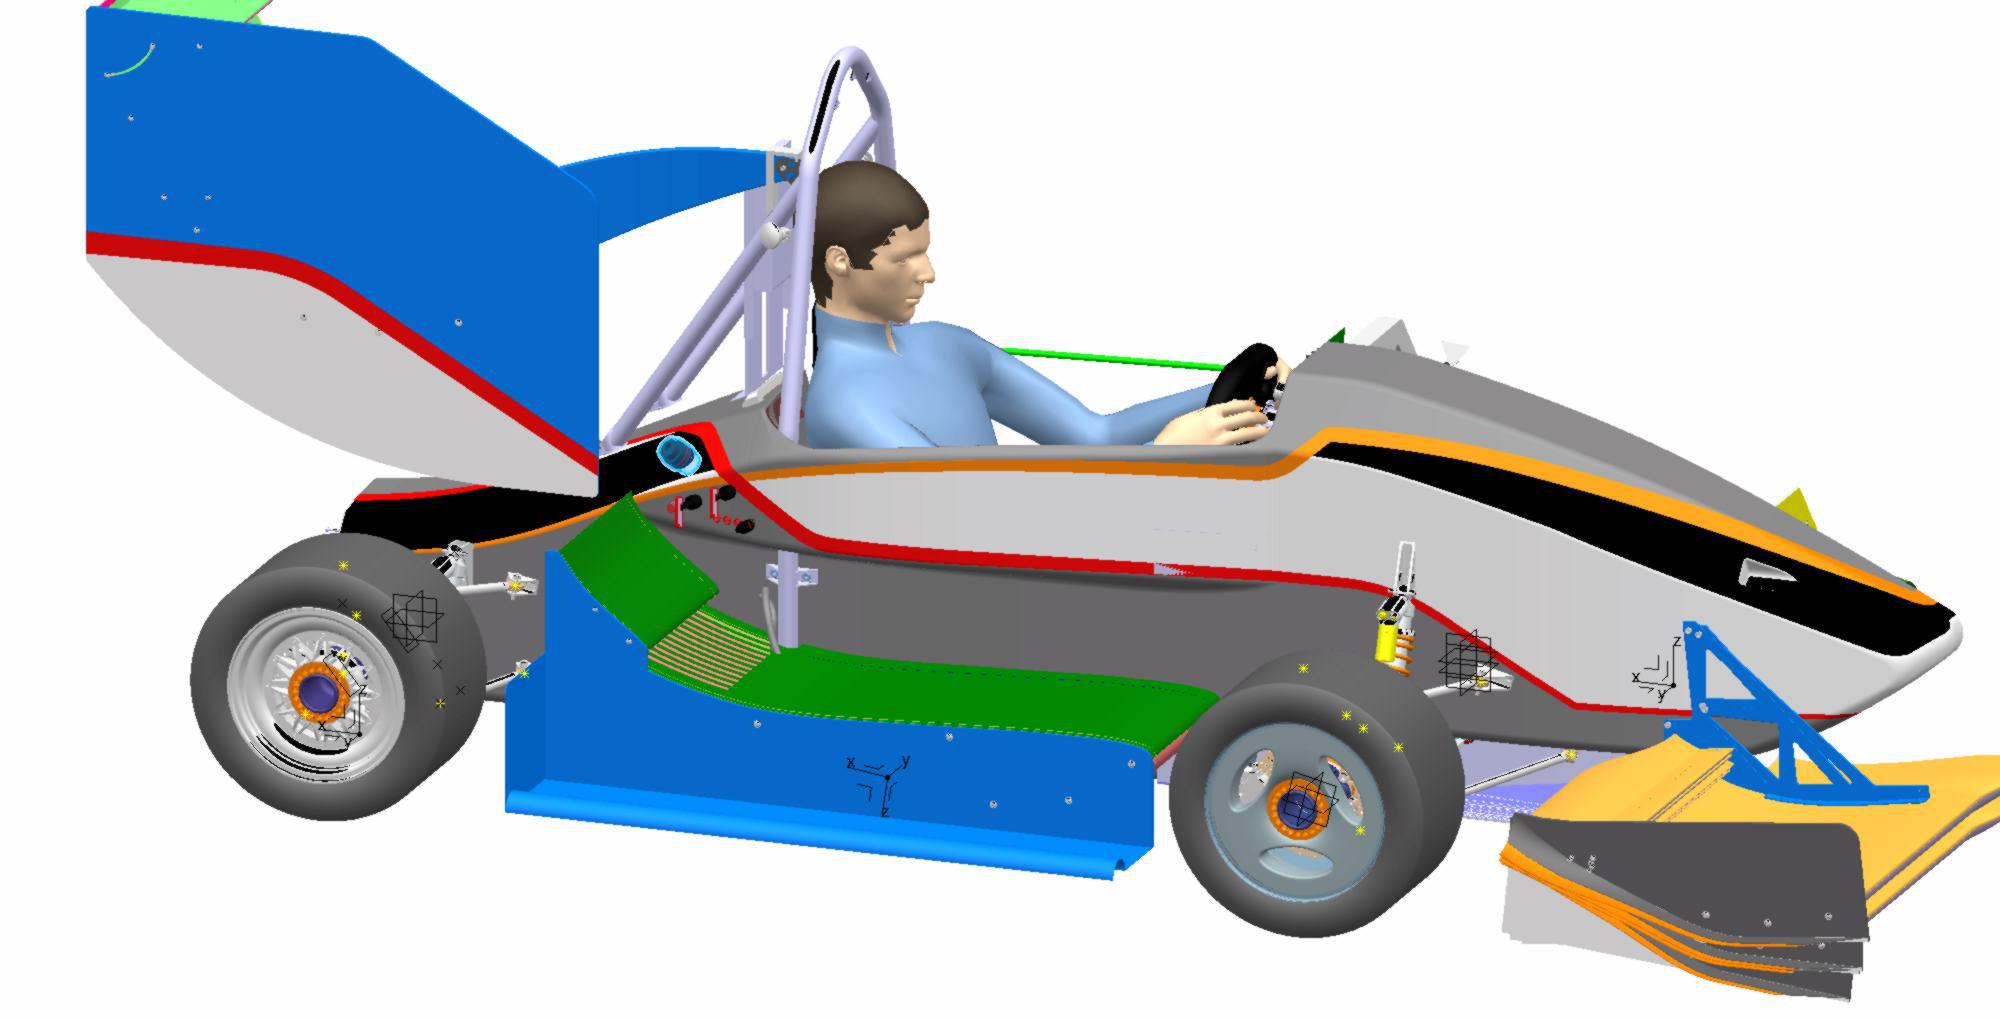
\includegraphics[width=\textwidth,trim={15cm 2cm 15cm 5cm},clip]{./img/hvd-position.jpg}
	\caption{HVD position.}
	\label{fig:hvd-position}
\end{figure}

\subsection{Ready-To-Drive-Sound (RTDS)}\label{subsec:RTDS}
%Responsible: Jano
% obrazky, schemata, rendery
% Dodelat odkazy a obrazky

\subsubsection{Description}
%Describe your concept of the RTDS, how the sound is produced, what are the parameters for activating the RTDS, etc.

We use piezo siren AE20M. The siren makes sound when ECUB recognize ready-to-drive state of car, it receives message from ECUF about TS ON button and SDC is in non-error state, if message would be lost ECUB doesn’t send confirmation status and ECUF does not allow to activate ready to drive status. Sound pressure level of this siren is more than 90 dB(A) at 1 m, Output frequency is from 2,9 kHz. Controlling of RTDS is done by ECUB by transistor. RTDS beeps 2 seconds.

\begin{figure}[H]
	\centering
	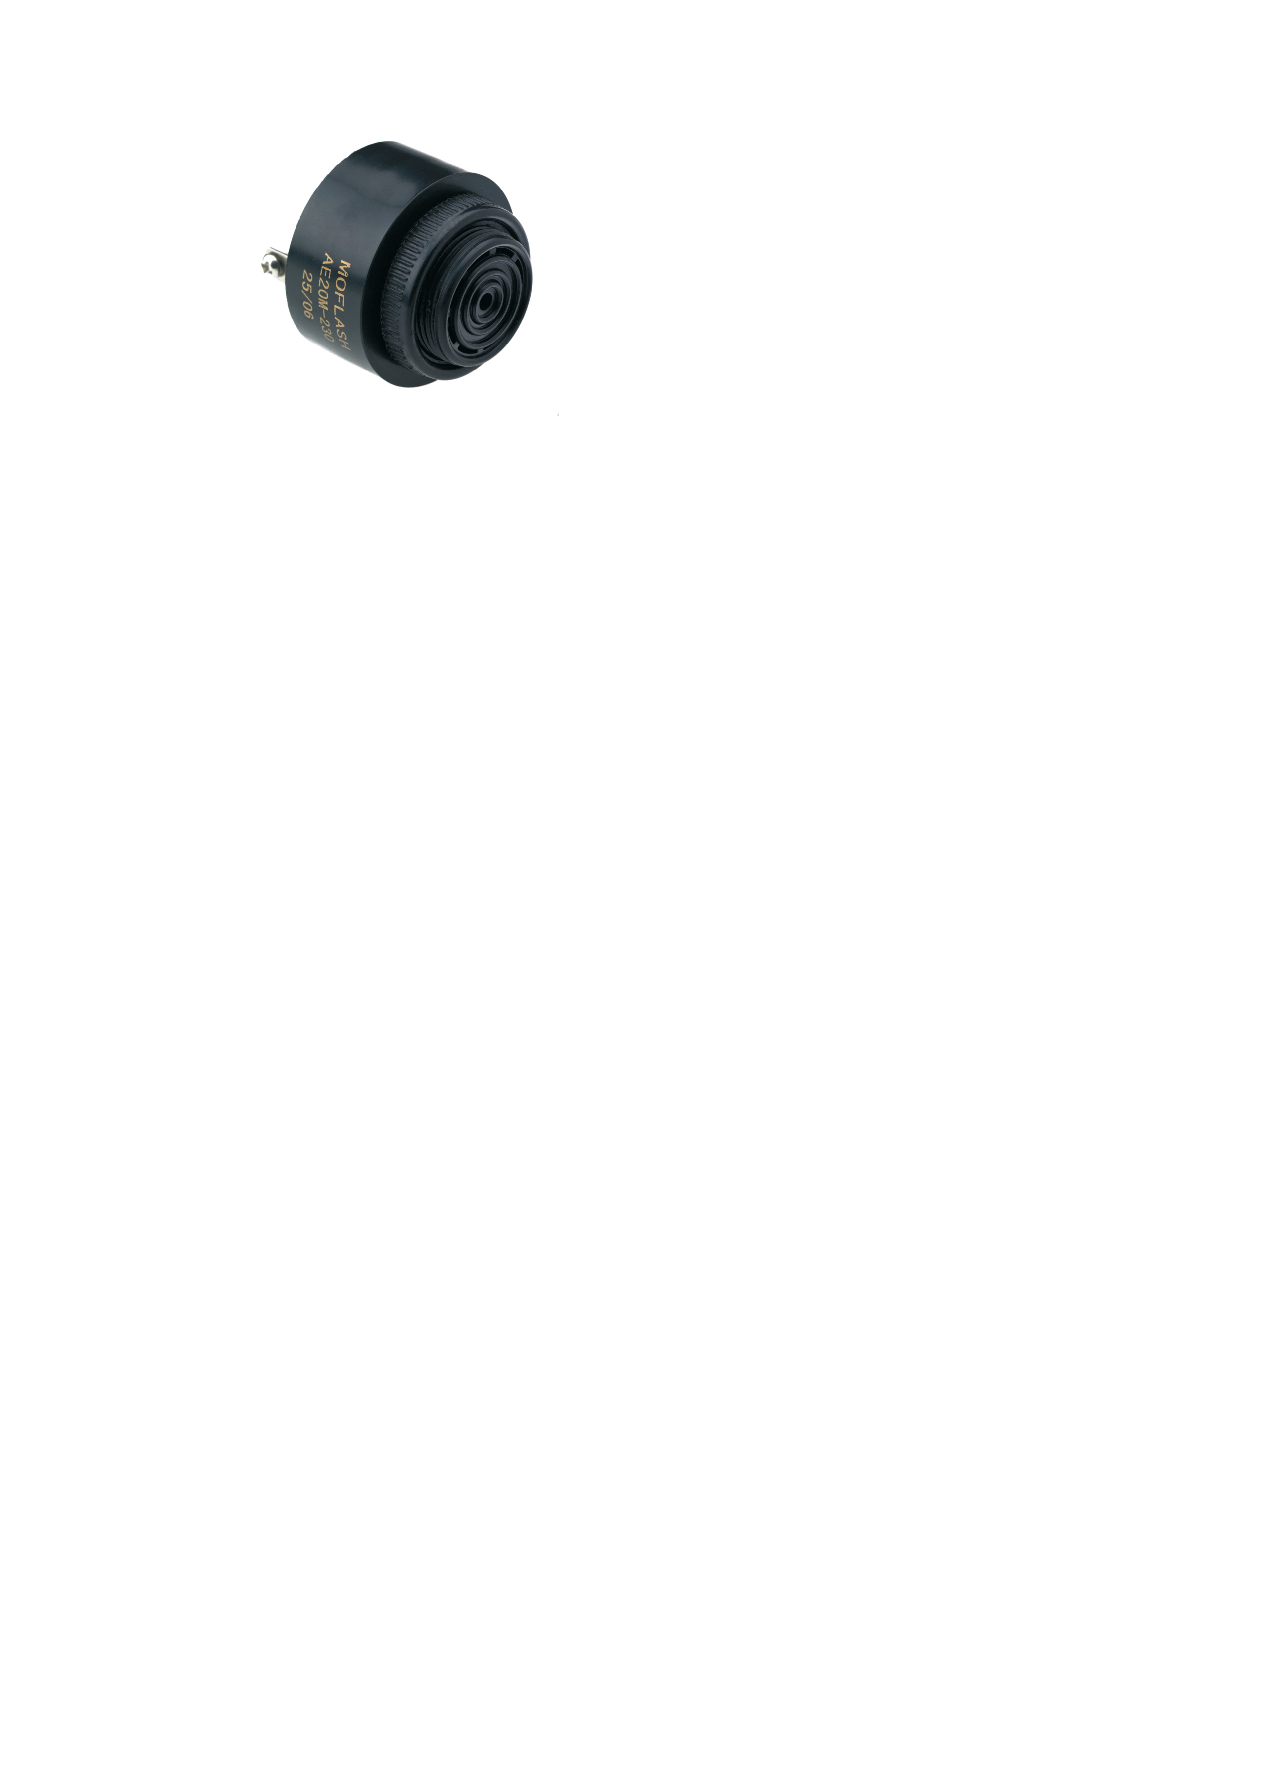
\includegraphics[width=.5\textwidth]{./img/RTDS.pdf}
	\caption{RTDS.}
	\label{fig:RTDS}
\end{figure}

\subsubsection{Wiring, cables, current calculations, connectors}
%Describe wiring, show schematics, describe connectors and cables and show useful data regarding the wiring.

There are only two wires from ECUB to RTDS piezo siren, one switched by transistor and and the second is ground (block connections is on \ref{fig:RTDS-wiring}).

\begin{figure}[H]
	\centering
	
\includegraphics[width=\textwidth]{./img/rtds-wiring.jpg}
	\caption{RTDS wiring.}
	\label{fig:RTDS-wiring}
\end{figure}
\subsubsection{Position in car}
%Provide CAD-renderings showing all relevant parts. Mark the parts in the rendering, if necessary.

Ready to drive sound is placed on the top of Accumulator Pack next to the Motor Controller, see \ref{fig:RTDS-position}.
\begin{figure}[H]
	\centering
	
\includegraphics[width=\textwidth]{./img/rtds-position.jpg}
	\caption{RTDS position.}
	\label{fig:RTDS-position}
\end{figure}

\newpage
\section{Accumulator}\label{sec:Accumualtor}
\subsection{HV Accumulator pack}\label{subsec:AccumulatorPack1}
%Responsible: Adam, JM
\subsubsection{Overview / description/parameters}
Describe concept of accumulator pack, provide table with main parameters like number of cells, cell stacks separated by maintenance plugs, cell configuration, resulting voltages->minimum, maximum, nominal, currents, capacity etc.
Fill out the following table:

\begin{table}[H]
	\centering
	\caption{Main accumulator parameters}
	\begin{tabularx}{\textwidth}{|X|X|}
		\hline
		Maximum Voltage: & 400 VDC \\[\TableSize]
		\hline
		Nominal Voltage: & 345.6 VDC \\[\TableSize]
		\hline
		Minimum Voltage: & 182 VDC \\[\TableSize]
		\hline
		Maximum output current: & 315 A (until any cell reaches 80 $^\circ$C) \\[\TableSize]
		\hline
		Maximum nominal current: & 270 A \\[\TableSize]
		\hline
		Maximum charging current: & 54 A \\[\TableSize]
		\hline
		Total numbers of cells: & 864 \\[\TableSize]
		\hline
		Cell configuration: & 96s9p \\[\TableSize]
		\hline
		Total Capacity: & 27.99 MJ \\[\TableSize]
		\hline
		Number of cell stacks < 120VDC & 6 \\[\TableSize]
		\hline
	\end{tabularx}%
	\label{tab:acc-main}%
\end{table}%

\subsubsection{Cell description}
Describe the cell type used and the chemistry, provide table with main parameters.
Fill out the following table:

\begin{table}[H]
	\centering
	\caption{Main cell specification}
	\begin{tabularx}{\textwidth}{|X|X|}
		\hline
		Cell Manufacturer and Type & SONY VTC5A \\[\TableSize]
		\hline
		Cell nominal capacity: & 2.5 Ah \\[\TableSize]
		\hline
		Maximum Voltage: & 4.25 V \\[\TableSize]
		\hline
		Nominal Voltage: & 3.6 V \\[\TableSize]
		\hline
		Minimum Voltage:  & 2 V \\[\TableSize]
		\hline
		Maximum output current: & 35 A (until cell reaches 80 $^\circ$C) (14C)\\[\TableSize]
		\hline
		Maximum nominal output current: & 30A(12C) \\[\TableSize]
		\hline
		Maximum charging current: & 6A(2.4C) \\[\TableSize]
		\hline
		Maximum Cell Temperature (discharging) & 80 $^\circ$C \\[\TableSize]
		\hline
		Maximum Cell Temperature (charging) & 60 $^\circ$C \\[\TableSize]
		\hline
		Cell chemistry: & Lithium-Ion \\[\TableSize]
		\hline
	\end{tabularx}%
	\label{tab:acc-cell}%
\end{table}%

\subsubsection{Cell configuration}
%Describe cell configuration, cell interconnect, show schematics of electrical configuration and CAD of connection techniques, cover additional parts like internal cell fuses etc.

Cell configuration is 96s9p. Cells are divided into 6 stacks, configuration of each stack is 16s9p. Cells are connected by welding. Main cells interconnection is done by nickel sheet. This sheet is welded to each cell. There is additional copper sheet welded over the nickel sheet (for lowering resistance of the main current path). 
\subsubsection{Cell temperature monitoring}
%Describe how the temperature of the cells is monitored, where the temperature sensors are placed, how many cells are monitored, etc. Show schematics, cover additional parts, etc.

The cells’ temperature is monitored by NTC temperature sensors. The manufacturer is TDK, type is: B57330V2103F260. Insulation of the sensors is done by 3M™ PTFE Film Electrical Tape. Breakdown voltage of this tape 9.5 kV, operating temperature is 180 $^\circ$C. Thickness of this tape is 0.1 mm. Sensors are soldered in PCBs that are covered with insulating tape and then mounted to each stack. 

Position of temperature sensors on the top of each stack (highlighted objects)
\begin{figure}[H]
	\centering
	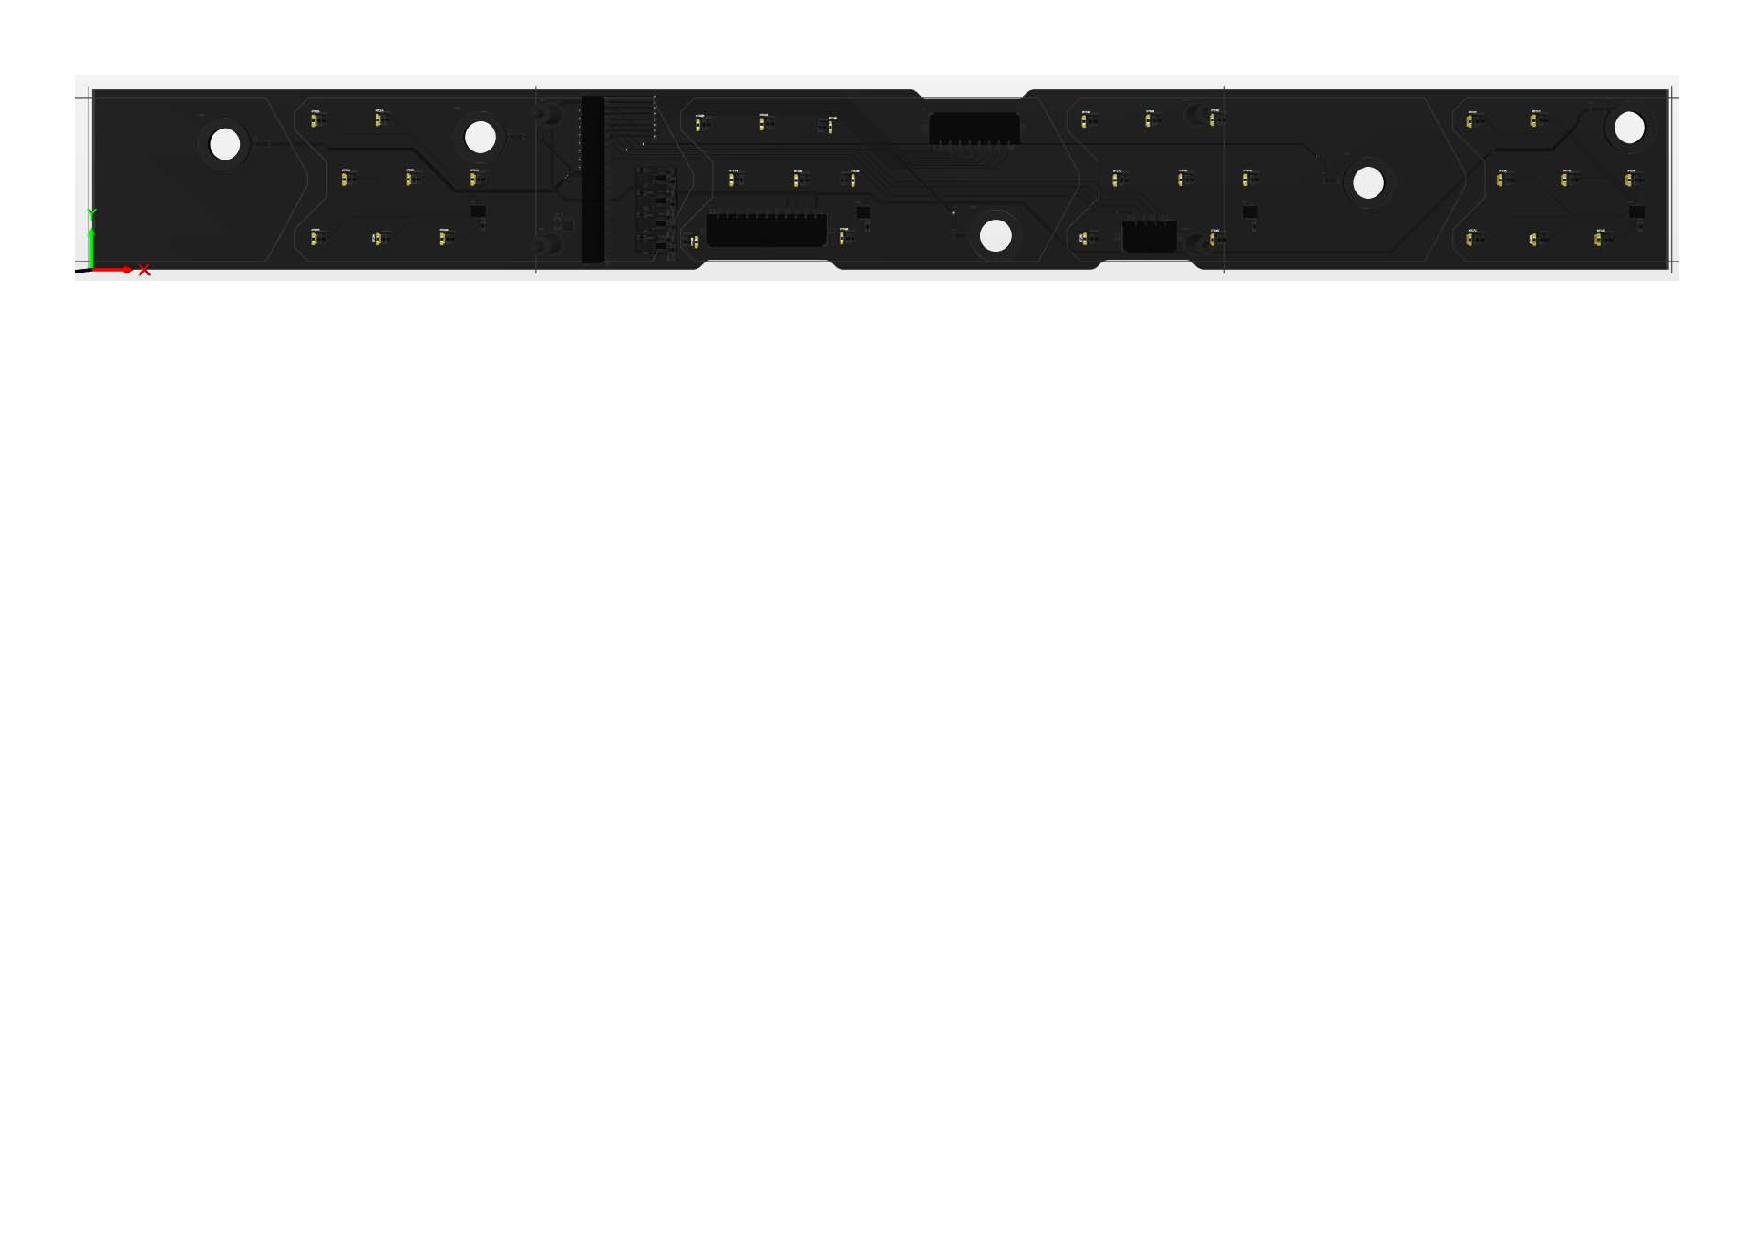
\includegraphics[width=\textwidth,trim={0cm 16cm 0cm 0cm}, clip]{./img/BMS-top-sensors.pdf}
	\caption{Top position of sensors.}
	\label{fig:BMS-top}
\end{figure}
Position of temperature sensors on the bottom of each stack (highlighted objects)
\begin{figure}[H]
	\centering
	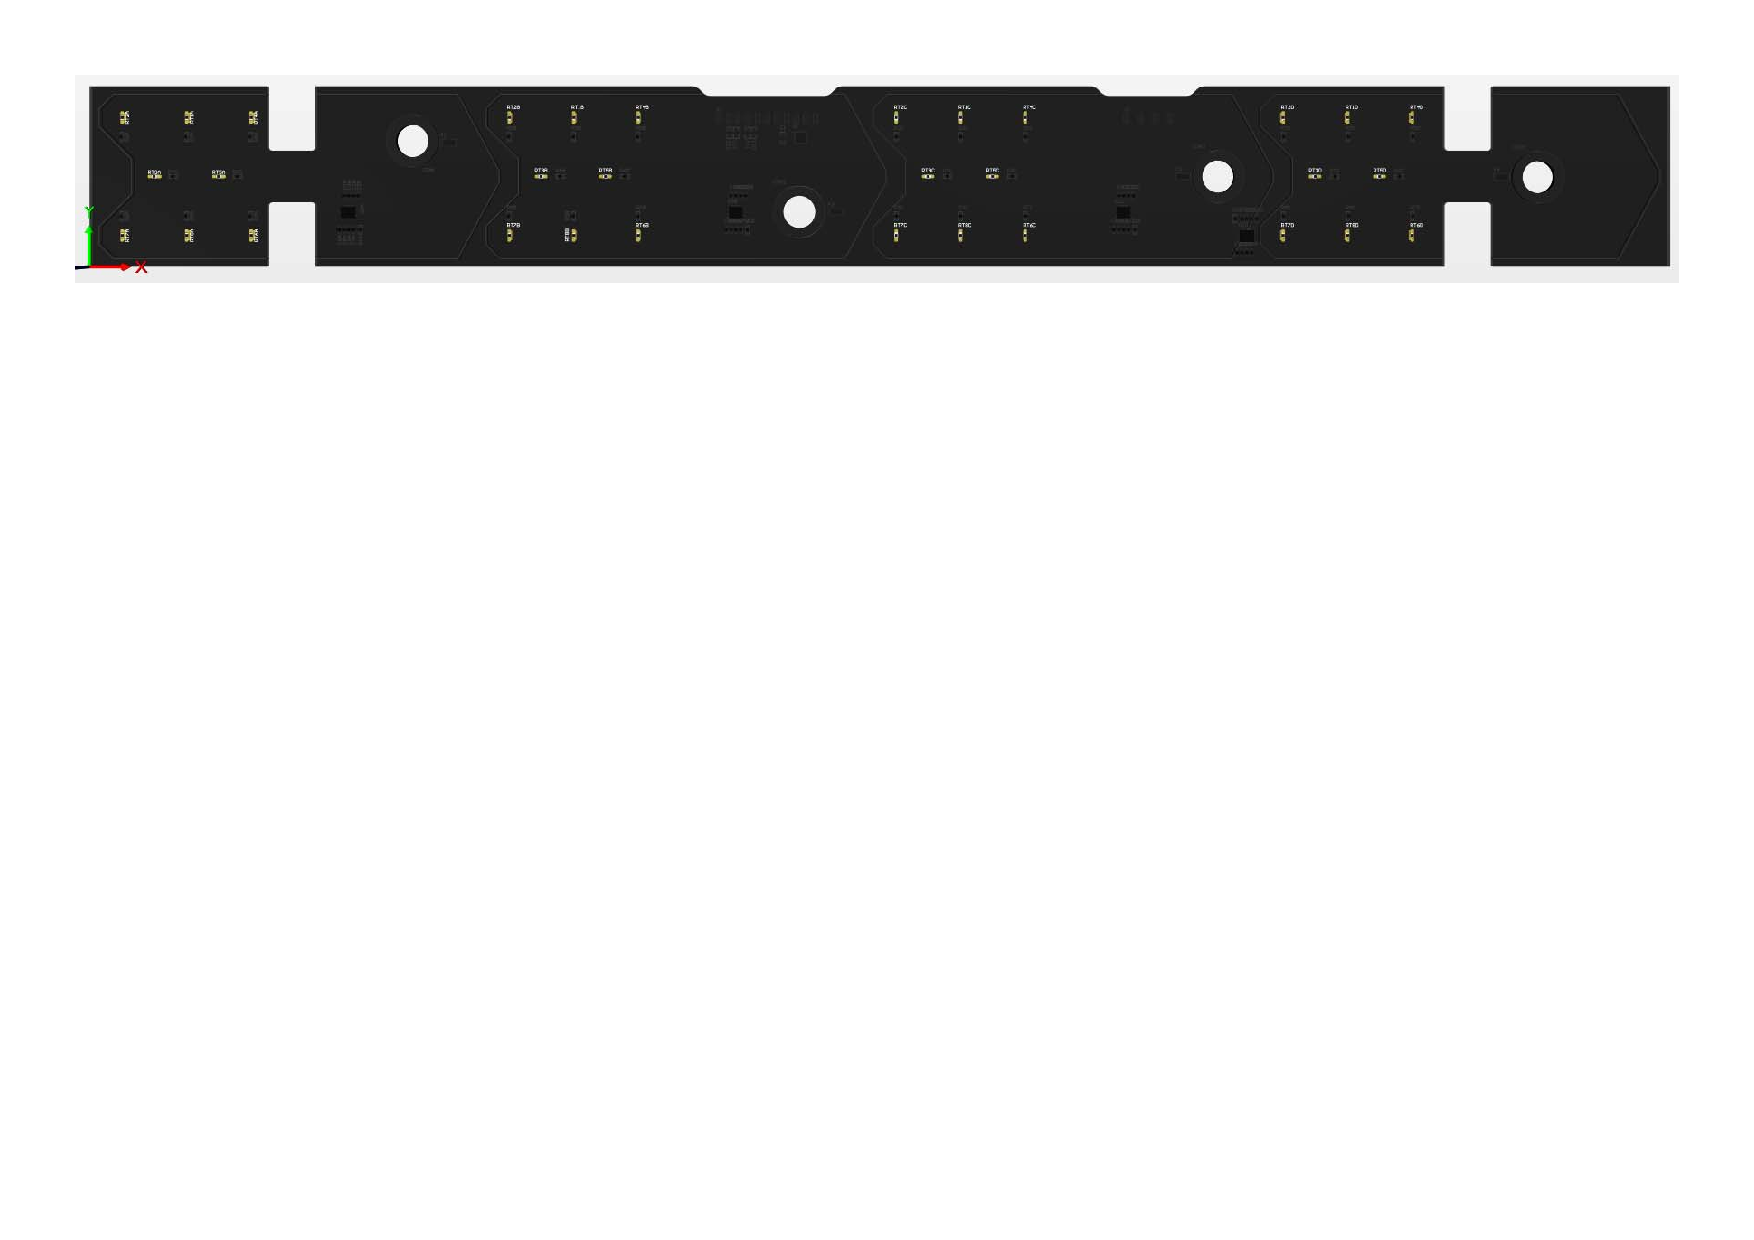
\includegraphics[width=\textwidth,trim={0cm 16cm 0cm 0cm}, clip]{./img/BMS-bottom-sensors.pdf}
	\caption{Bottom position of sensors.}
	\label{fig:bms-bottom}
\end{figure}
Top and bottom view of one stack 
\begin{figure}[H]
	\centering
	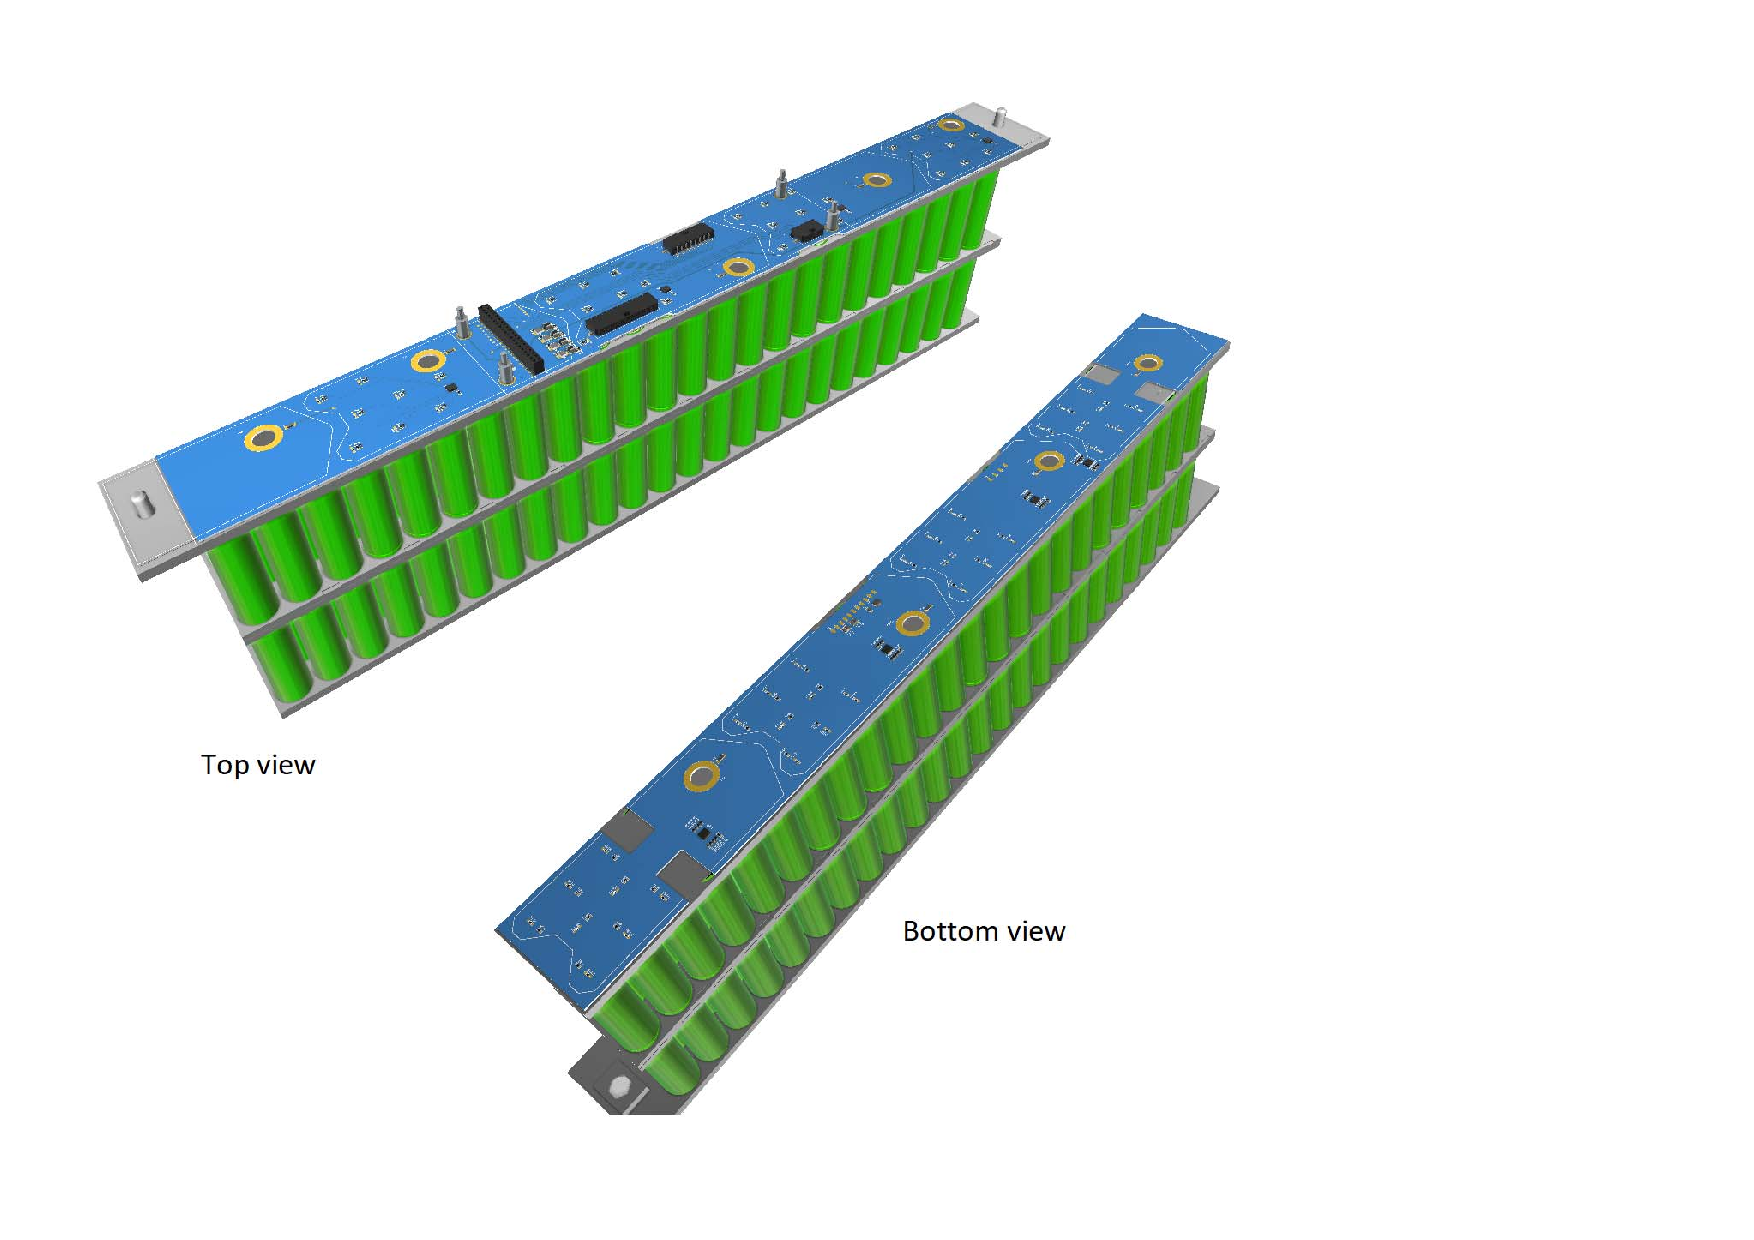
\includegraphics[width=\textwidth]{./img/BMS-top-andbottom.pdf}
	\caption{Rear and bottom view.}
	\label{fig:torque1}
\end{figure}

\begin{table}[H]
	\centering
	\caption{General cell temperature parameters.}
	\begin{tabularx}{\textwidth}{|X|X|}
		\hline
		Temperature sensor accuracy: & 1\% \\[\TableSize]
		\hline
		Total number of cells: & 864 \\[\TableSize]
		\hline
		Total number of sensors: &  384 \\[\TableSize]
		\hline
		Max. distance from monitored negative cell terminal: & 2 mm \\[\TableSize]
		\hline
		AMS opens AIRs during dis-charging if cell temperature is above: & 60$^\circ$C \\[\TableSize]
		\hline
		AMS opens AIRs during charging if cell temperature is above: & 60$^\circ$C \\[\TableSize]
		\hline
	\end{tabularx}%
	\label{tab:acc-temp}%
\end{table}%

\subsubsection{Acumulator Managment System}
Describe the AMS used including at least the following:

% Table generated by Excel2LaTeX from sheet 'List1'
\begin{table}[H]
	\centering
	\caption{Cell voltage limits.}
	\begin{tabularx}{\textwidth}{|X|X|}
		\hline
		Minimum cell voltage (shutdown limit): & 2.2 V \\[\TableSize]
		\hline
		Maximum cell voltage (shutdown limit): & 4.2 V \\[\TableSize]
		\hline
		Measurement precision (mV): & $\pm$ 0.75 \\[\TableSize]
		\hline
	\end{tabularx}%
	\label{tab:acc-limits}%
\end{table}%
\iffalse
\begin{itemize}
	\item 	Sense wiring protection (fusing / fusible link wire used)
	\item What upper and lower voltage does the AMS react at and how does it react?
	\item What cell temperature does the AMS react at and how does it react?
	\item Show tables of operation parameters
	\item Describe how many cells are sensed by each AMS board, the configuration of the cells, the configuration of the boards and how any comms wiring between boards is protected 
	\item Describe how the AMS is able to open the AIRs if any error is detected
	\item Describe where galvanic isolation occurs between TS and GLV system connections.
\end{itemize}\fi
Each sense connection is protected with fuse. There are two types of fuses used: 

\noindent Littelfuse 0251001.MXL (Those are used, where the cells are contacted via PCB)

\noindent Eaton TR/3216LV1-R (Those are used, where measure wires are connected directly to cells)

Cell highest allowed voltage is 4.25 V so AMS reacts when the voltage is above 4.2 V. Cell lowest allowed voltage is 2 V so AMS reacts when the voltage is below 2.2 V. Reaching any of limits causes AIRs disconnection.

Highest allowed temperature (by datasheet) for discharging is 80 $^\circ$C and for charging 60 $^\circ$C. Due to FSE rules our battery pack is limited to 60 $^\circ$C. AMS reacts when the temperature is higher than 60 $^\circ$C reaching limit causes AIRs disconnection.

\paragraph{Recommended Operating Conditions}
TA = 25°C and TOP = 57.6 V; Min/Max values stated where TA = –40°C to 105⁰C and TOP = 12 V to 79.2 V (unless otherwise noted)
\begin{figure}[H]
	\centering
	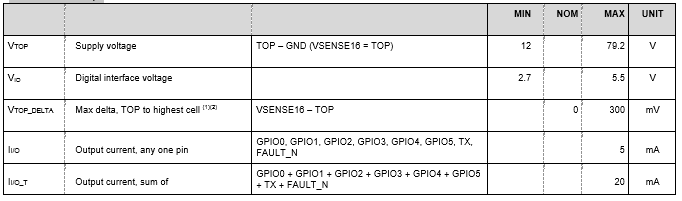
\includegraphics[width=\textwidth]{./img/BMS-operatingparms.png}
	\caption{Recomended operating parameters.}
	\label{fig:BMS-op-params}
\end{figure}


Each AMS board senses whole stack, that means it senses 144 cells, connected in 16s9p configuration. Comms wirings are protected by two 1kV 1nF capacitors CC1206KKX7RCBB102 by Yageo. There is placed one on each side (there is one on every AMS). The AMS is connected to Accumulator ECU that has capability of direct AIRs shutdown. The galvanic isolation between TS and GLV is done by two 1kV 1nF capacitors CC1206KKX7RCBB102 by Yageo. It is located on separated board connected between first AMS and Accumulator ECU.




\subsubsection{Accumulator indicator}
Describe the indicator, show wiring, provide tables with operation, PCB design, etc

\subsubsection{Wiring, cables, current calculations, connectors}
Describe the internal wiring, show schematics, provide calculations for currents and voltages and show data regarding the cables and connectors used.
\begin{itemize}
	\item 	Discuss maximum expected current, DC and AC how long will this be provided?
	\item Compare the maximum values to nominal currents
	\item Give a table for each kind of wire in your tractive-system:
	\item Describe your maintenance plugs, provide pictures
	\item Use tables like the one shown below:
\end{itemize}

% Table generated by Excel2LaTeX from sheet 'List1'
\begin{table}[htbp]
	\centering
	\caption{Wire data of company A, 0.205 mm$^2$.}
	\begin{tabularx}{\textwidth}{|X|X|}\hline
		Wire type &  \\[\TableSize]\hline
		Continuous current rating: &  \\[\TableSize]\hline
		Cross-sectional area &  \\[\TableSize]\hline
		Maximum operating voltage: &  \\[\TableSize]\hline
		Temperature rating: &  \\[\TableSize]\hline
		Wire connects the following components: &  \\[\TableSize]\hline
	\end{tabularx}%
	\label{tab:acc-wire}%
\end{table}%

\subsubsection{Accumualtor insulation relays}
Describe the AIRs used and their main operation parameters, use tables, etc.
Additionally, fill out the following table:

% Table generated by Excel2LaTeX from sheet 'List1'
\begin{table}[H]
	\centering
	\caption{Basic AIR data.}
	\begin{tabularx}{\textwidth}{|X|X|}
		\hline
		Relay Type: &  \\[\TableSize]
		\hline
		Contact arragment: &  \\[\TableSize]
		\hline
		Continous DC current rating: &  \\[\TableSize]
		\hline
		Overload DC current rating:  &  \\[\TableSize]
		\hline
		Maximum operation voltage: &  \\[\TableSize]
		\hline
		Nominal coil voltage: &  \\[\TableSize]
		\hline
		Normal Load switching: & \\[\TableSize]
		\hline
		Maximum Load switching &  \\[\TableSize]
		\hline
	\end{tabularx}%
	\label{tab:acc-air}%
\end{table}%

\subsubsection{Fusing}
Describe the fuses used and their main operation parameters, use tables, etc.
Additionally, fill out the following table for each fuse type used:

\begin{table}[H]
	\centering
	\caption{Basic fuse data}
	\begin{tabularx}{\textwidth}{|X|X|}
		\hline
		Fuse manufacturer and type: &  \\[\TableSize]
		\hline
		Continous current rating:  &  \\[\TableSize]
		\hline
		Maximum operating voltage  &  \\[\TableSize]
		\hline
		Type of fuse: &  \\[\TableSize]
		\hline
		I2t rating: &  \\[\TableSize]
		\hline
		Interrupt Current (maximum current at which the fuse can interrupt the current) &  \\[\TableSize]
		\hline
	\end{tabularx}%
	\label{tab:acc-fuse}%
\end{table}%

Create a table with components and wires protected by the fuse(s) and the according continuous current rating, below is an example table with some potential entries.  Complete this table with information for your design and add/remove additional locations as applicable.  Ensure that the rating of all the components is greater than the rating of the fuse such that none of the other components become the fuse.

% Table generated by Excel2LaTeX from sheet 'List1'
\begin{table}[H]
	\centering
	\caption{Fuse Protection Table}
	\begin{tabularx}{\textwidth}{|X|X|X|X|X|}
		\hline
		Location & Wire Size & Wire Ampacity & Fuse type & Fuse rating\\[\TableSize]
		\hline
		Cells to AIRs & 2 AWG & XXX & MNO Fuse & XXX \\[\TableSize]
		\hline
		AIR to Motor controller & 0 AWG & XXX & 2x MNO Fuse & XXX \\[\TableSize]
		\hline
		AIR to TSAL & 20 AWG & XXX & EFG Fuse & XXX \\[\TableSize]
		\hline
		Accumulator output connector & 2 AWG & XXX &     &  \\[\TableSize]
		\hline
		Cells to AMS &     &     &     &  \\[\TableSize]
		\hline
	\end{tabularx}%
	\label{tab:acc-fuse-protection}%
\end{table}%

\subsubsection{Charging}
Describe how the accumulator will be charged. How will the charger be connected? How will the accumulator be supervised during charging? Show schematics, CAD-Renderings, etc., if needed
Additionally, fill out the table:

\begin{table}[H]
	\centering
	\caption{General charger data}
	\begin{tabularx}{\textwidth}{|X|X|}
		\hline
		Charger Type: & \\[\TableSize]
		\hline
		Maximum charging power: &\\[\TableSize]
		\hline
		Maximum charging voltage: &  \\[\TableSize]
		\hline
		Maximum charging current: &  \\[\TableSize]
		\hline
		Interface with accumulator &  \\[\TableSize]
		\hline
		Input voltage: & \\[\TableSize]
		\hline
		Input current: &  \\[\TableSize]
		\hline
	\end{tabularx}%
	\label{tab:acc-charger}%
\end{table}%

\subsubsection{Mechanical Configuration/materials}
Describe the concept of the container, show how the cells are mounted, use CAD-Renderings, show data regarding materials used, etc.

\subsubsection{Position in car}
Provide CAD-renderings showing the relevant parts. Mark the parts in the rendering, if necessary.  Ensure that the required mechanical structure to protect the accumulator and other electrical components is clearly identified.








\subsection{GLVS Accmulator}
\subsubsection{Description}
Describe your concept of the GLVS Accumulator.

\subsubsection{Wiring, cables, current calculations, connectors}
Describe wiring, show schematics, describe connectors and cables and show useful data regarding the wiring.  Include information on the working voltage and current rating of the accumulator.

\begin{table}[H]
	\centering
	\caption{GLVS accumualtor general parameters.}
	\begin{tabularx}{\textwidth}{|X|X|}\hline
		Cell/Accumulator: & Li-ion\\[\TableSize]\hline
		Accumulator configuration – parallel: & 1 \\[\TableSize]\hline
		Accumulator configuration – series: & 6 \\[\TableSize]\hline
		Maximum Voltage: & 25.5 V \\[\TableSize]\hline
		Nominal Voltage: & 21.6V \\[\TableSize]\hline
		Minimum Voltage: & 12V \\[\TableSize]\hline
		Max. Continuous Discharge Current: &  \\[\TableSize]\hline
		Peak Discharge Current: &  \\[\TableSize]\hline
		Peak Discharge Current Time: &  \\[\TableSize]\hline
		Max. Continuous Charge Current &  \\[\TableSize]\hline
		Total capacity[MJ]: &  \\[\TableSize]\hline
	\end{tabularx}%
	\label{tab:LVbatt-general}%
\end{table}%

\subsubsection{Position in car}
Provide CAD-renderings showing all relevant parts. Mark the parts in the rendering, if necessary.

\newpage
\section{Energy meter mounting}\label{sec:DataLogger}
%Responsible: Kosina
\subsection{Description}
Describe where the energy meter is mounted and how, etc.

\subsection{Wiring, cables, current calculations, connectors}
Describe the wiring, show schematics, provide calculations for currents and voltages, and show data regarding the cables and connectors used.

\subsection{Position in car}
%Provide CAD-renderings showing all relevant parts. Mark the parts in the rendering, if necessary.

\begin{figure}[H]
	\centering
	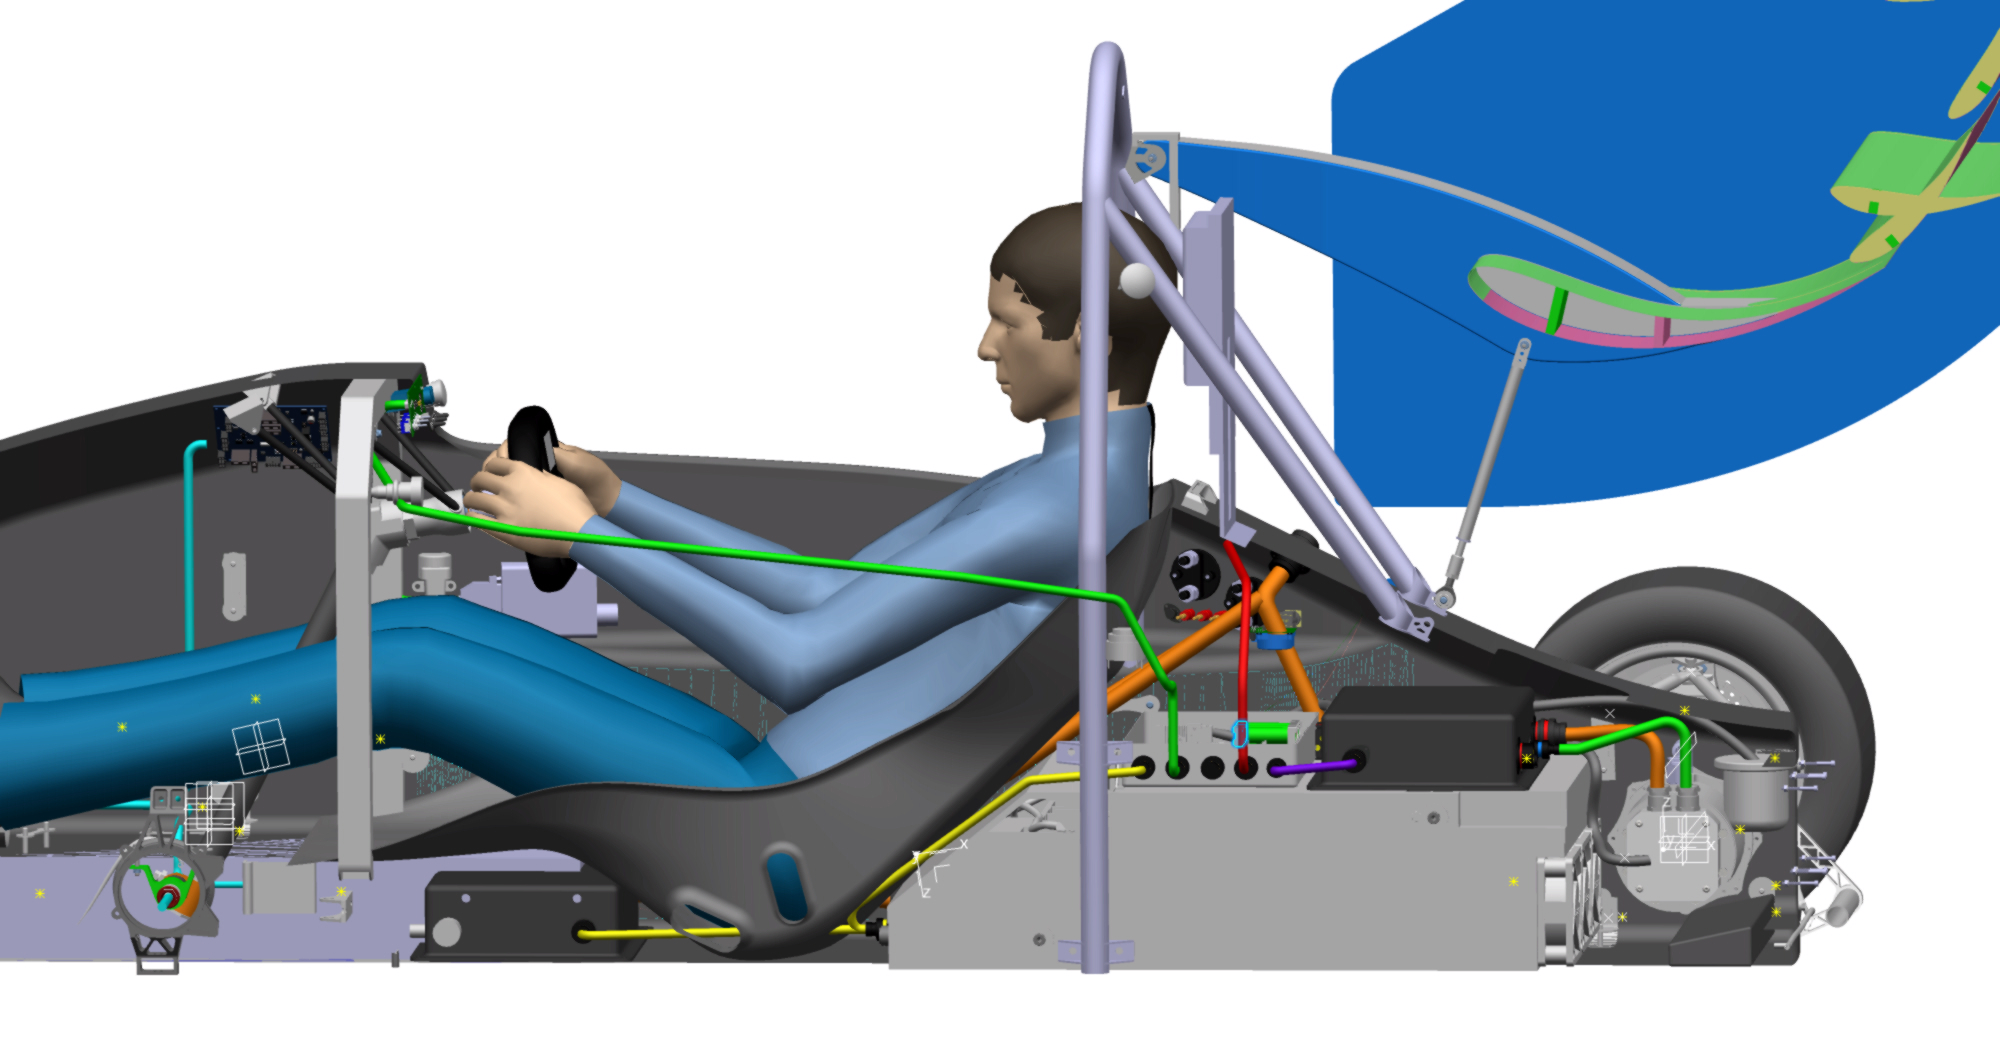
\includegraphics[width=.5\textwidth]{./img/ServiceBox-position.jpg}
	\caption{Service box position.}
	\label{fig:ServiceBox-position}
\end{figure}







\newpage
\section{Motor Controller}\label{sec:MotorController}
%Res:Hotovo
%Kontrola kabelaze
\subsection{Motor Controller 1}
% Kabeláž
% add schematic and datasheet

\subsubsection{Description, type, operation parameters}
%Describe important functions; provide table with main parameters like resulting voltages->minimum, maximum, nominal, currents etc.
Motor controller is a prototype of MiRy X-Boss Motor Controller. It is fully self-designed for driving 2 PMSM motors simultaneously with Resolver sensors as a position feedback. Field Oriented Control is implemented with galvanic isolated current sensors LEM HTFS 200-P.

Galvanic isolation on PCB is shown in \ref{app:mc-top} and \ref{app:mc-bot}. The only place where isolation is smaller then required 4mm is between pins of DC/DC NME1215SC. Real space gap is 1.54mm. The NME1215SC has rated voltage of 1kV. See \ref{app:NME1215SC}.

Motor Controller communicate with traction control unit by private CAN bus. If any error occurs in their communication – Motor Controller stops driving both motors (error mode). It also implements discharge circuit which is activated by CAN or in case of Auxiliary supply disconnection (resistors are driven by normally-closed relay).

A current limit is set to not overload used motors. For each motor controller different. Rear motor controller has set peak current limit to 202A and temperature limit to 120°C. Front Motor Controller’s current limit is 70A and temperature limit also 120$\circ$C.

\begin{table}[H]
	\centering
	\caption{General motor controller data}
	\begin{tabularx}{\textwidth}{|X|X|}\hline
		Motor controller type: & MiRy X-Boss \\[\TableSize]\hline
		Maximum continous power: & 2 x 90kW (in:400V, out:200A) \\[\TableSize]\hline
		Maximum peak power: & 2 x 146kW for 5s (in:400V, out:300A) \\[\TableSize]\hline
		Maximum Input voltage: & 410VDC \\[\TableSize]\hline
		Output voltage: & 282 VAC \\[\TableSize]\hline
		Maximum continuous output current: & 2 x 200A \\[\TableSize]\hline
		Maximum peak current: & 2 x 300A for 5s \\[\TableSize]\hline
		Control method: & CAN \\[\TableSize]\hline
		Cooling method: & Water \\[\TableSize]\hline
		Auxiliary supply voltage: & 24VDC \\[\TableSize]\hline
	\end{tabularx}%
	\label{tab:MC:general}%
\end{table}%

\subsubsection{Wiring, cables, current calculations, connectors}
%Describe the wiring, show schematics, provide calculations for currents and voltages and show data regarding the cables and connectors used.

Motor controllers are connected with HVD box by high voltage cable. High current connector “ASHD 0 22-24320 P N” by Deutsch is used. 

\begin{table}[H]
	\centering
	\caption{Wire data of Raychem TR-16-16$^2$}
	\begin{tabularx}{\textwidth}{|X|X|}\hline
		Wire type: & Raychem TR-16-16  \\[\TableSize]\hline
		Current rating: & 100A \\[\TableSize]\hline
		Fuse current rating: & ??? \\[\TableSize]\hline
		Maximum operating voltage: & 600V \\[\TableSize]\hline
		Temperature rating: & 125 °C \\[\TableSize]\hline
	\end{tabularx}%
	\label{tab:MC:wire}%
\end{table}%

%table
\subsubsection{Position in car}
%Provide CAD-renderings showing the relevant parts. Mark the parts in the rendering, if necessary.

The position of both motor controllers is shown in \ref{fig:MC:position}.

\begin{figure}[H]
	\centering
	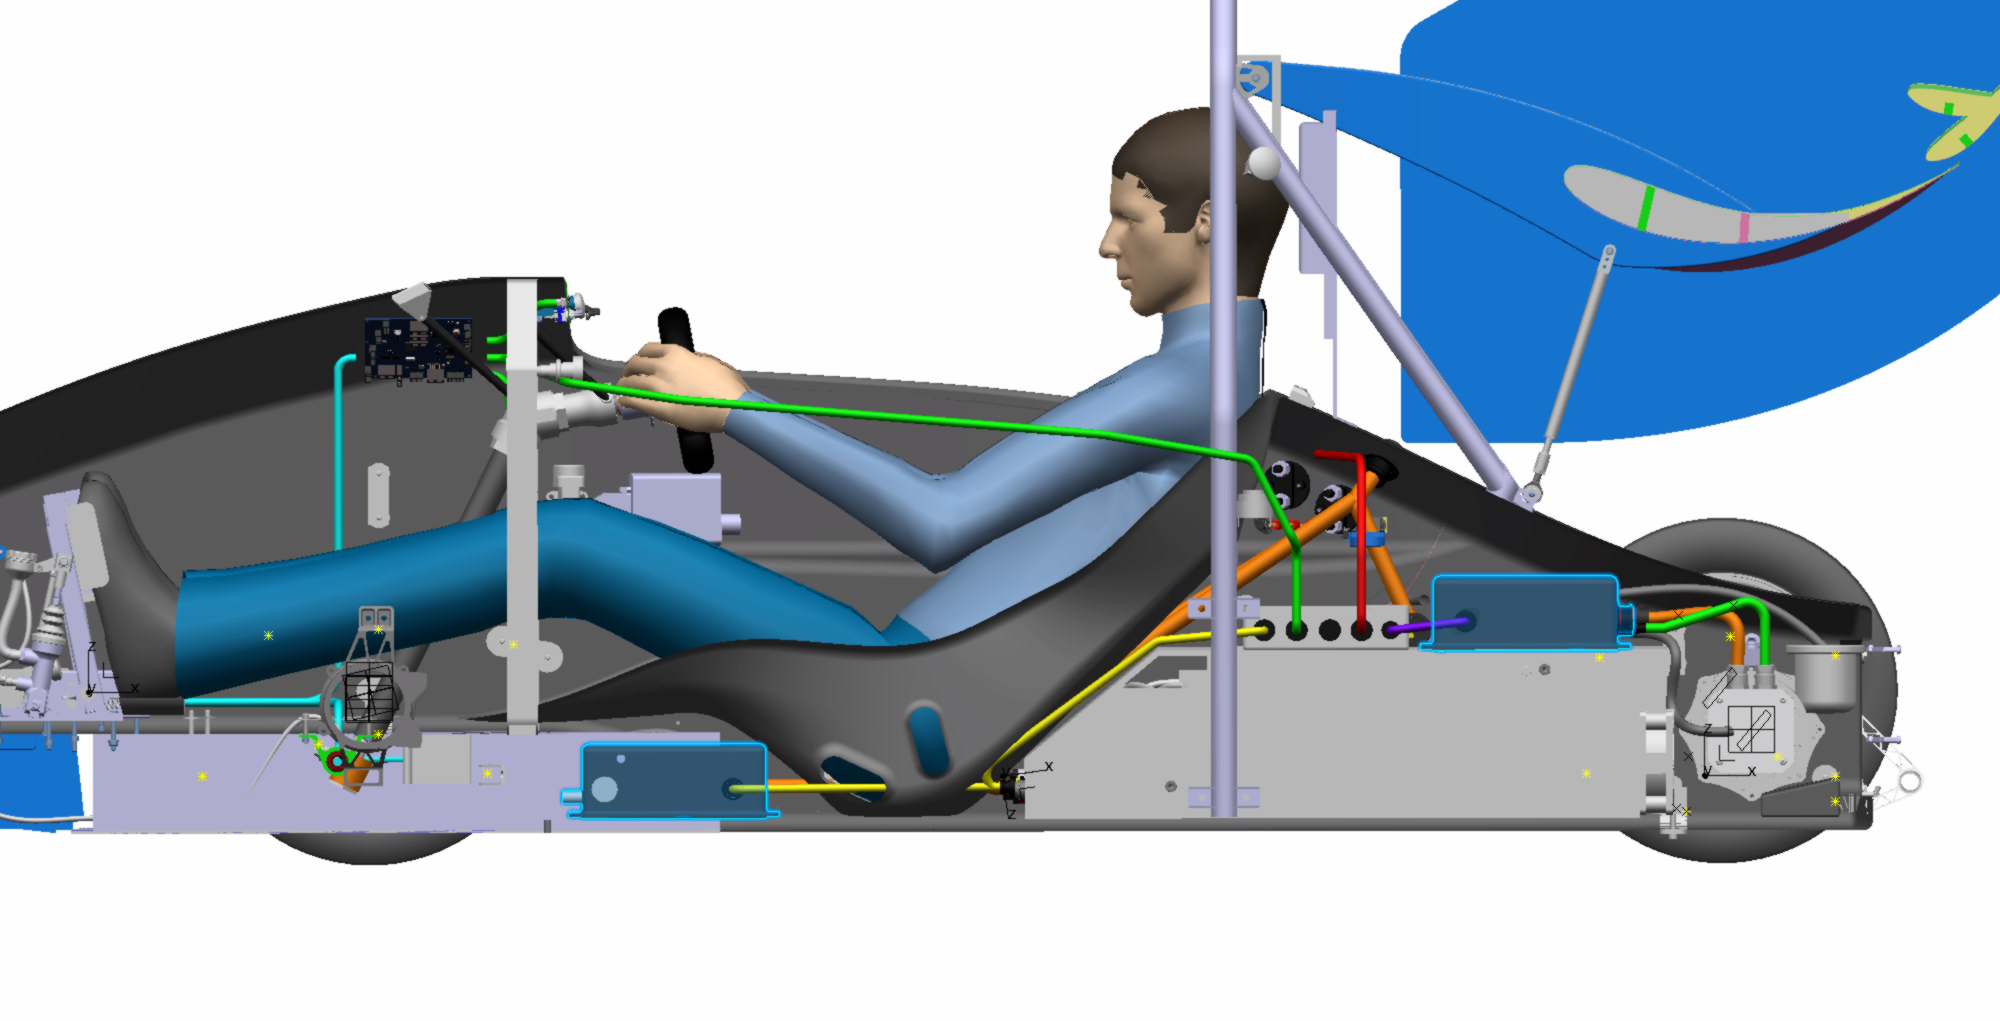
\includegraphics[width=\textwidth]{./img/MC-position.jpg}
	\caption{MC position.}
	\label{fig:MC:position}
\end{figure}
\subsection{Motor Controller 2}
%If identical parts are used, just refer to the corresponding sections, don’t copy and paste.
Motor controller 2 is identical as Motor controller 1.






\newpage
\section{Motors}\label{sec:Motors}
%res: Nove datasheet
%Kontrola ale nakopirovano
\subsection{Motor 1}

\subsubsection{Description, type, operation parameters}
%Describe the motor used, provide table with main parameters like resulting voltages->minimum, maximum, nominal, currents, resulting motor power, use figures to show important characteristics.

We are using prototype motors from company TG Drives. They developed prototype motors with special parameters and water cooling. We are using two motors on rear axle (motor 1) and two motors on front axle.
\begin{table}[H]
	\centering
	\caption{General motor 1 data}
	\begin{tabularx}{\textwidth}{|X|X|}\hline
		Motor Manufacturer and Type: & TG Drives – N5-1600-100-380a-h-special-v2 \\[\TableSize]\hline
		Motor principle & PMSM \\[\TableSize]\hline
		Maximum continuous power: & 11.5 kW \\[\TableSize]\hline
		Peak power: & 35 kW \\[\TableSize]\hline
		Input voltage: & 260 VAC \\[\TableSize]\hline
		Nominal current: & 38.2 A \\[\TableSize]\hline
		Peak current: & 171 A \\[\TableSize]\hline
		Maximum torque: & 48 Nm \\[\TableSize]\hline
		Nominal torque: & 11 Nm \\[\TableSize]\hline
		Cooling method: & Water \\[\TableSize]\hline
	\end{tabularx}%
	\label{tab:motors1-general}%
\end{table}%

\begin{figure}[H]
	\centering
	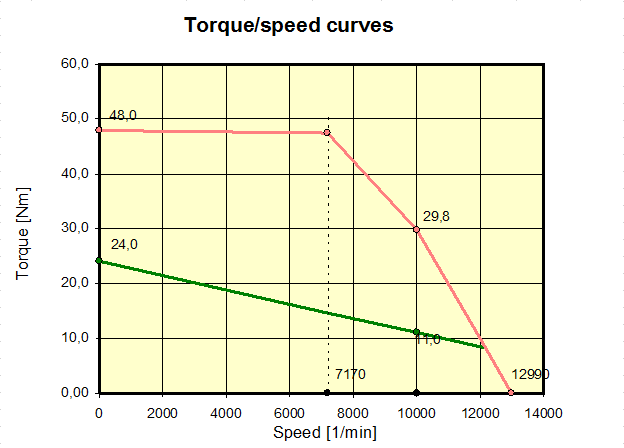
\includegraphics[width=\textwidth]{./img/MOTOR1-torque.png}
	\caption{Rear motor characteristics.}
	\label{fig:torque1}
\end{figure}

\iffalse\begin{itemize}
\item 	Give a plot of power vs. Rpm including a line for nominal and maximum power
\item give a plot of torque vs. rpm including a line for nominal and maximum torque
\end{itemize}\fi

\subsubsection{Wiring, cables, current calculations, connectors}
We use Raychem TR 16-10-0 and TR 16-6-0. There are leadthrough used for cables in motors and connectors Souriau „8STA 0 18 18” are used in Motor controllers.

\subsubsection{Position in car}
%Provide CAD-renderings showing all relevant parts. Mark the parts in the rendering, if necessary and clearly identify the structure used to protect all relevant parts.

Rear motors are situated in the rear-most part of the frame. 

\begin{figure}[H]
	\centering
	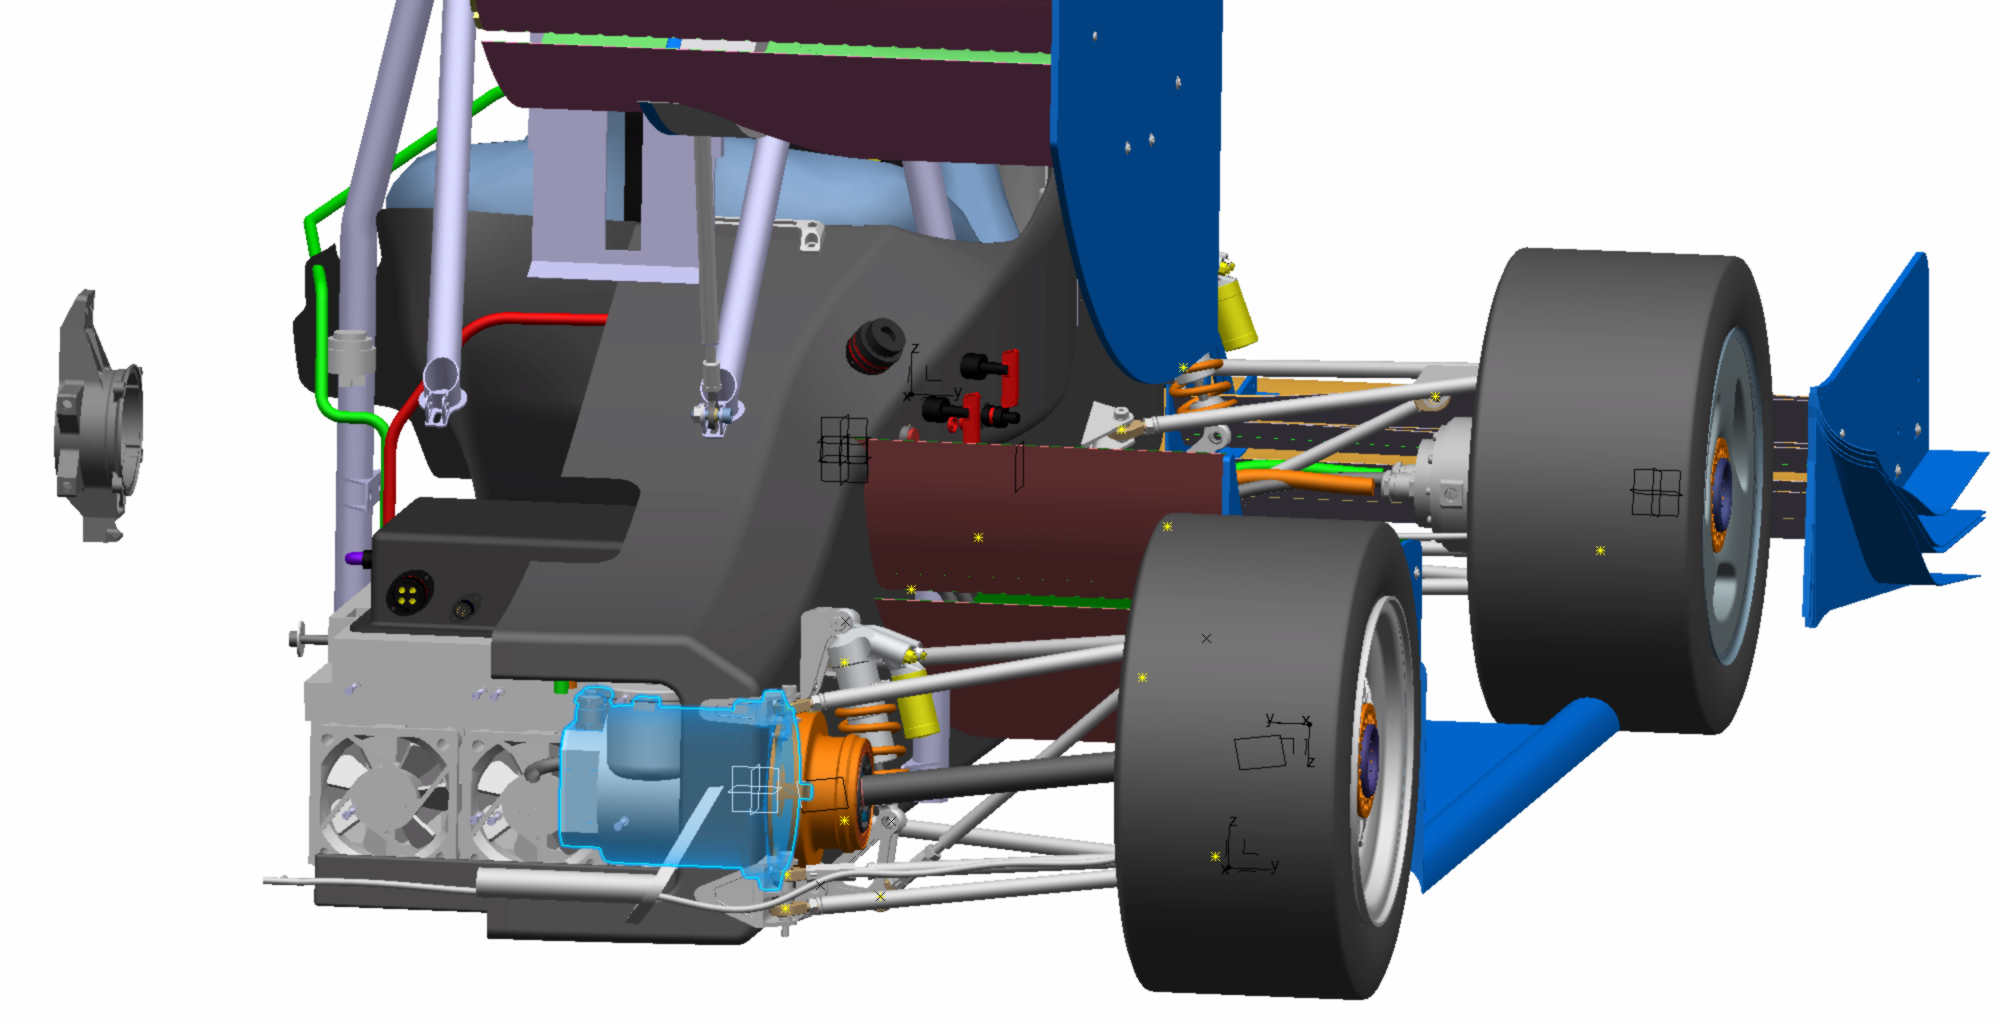
\includegraphics[width=\textwidth]{./img/Motor-rear-position.jpg}
	\caption{Rear motor position.}
	\label{fig:Motor-rear-position}
\end{figure}

\subsection{Motor 2}% Front

\begin{table}[H]
	\centering
	\caption{General motor 2 data}
	\begin{tabularx}{\textwidth}{|X|X|}\hline
		Motor Manufacturer and Type: & TG Drives – M4-0470-90-380a-h-special-water-cooling-lfe-60mm \\[\TableSize]\hline
		Motor principle & PMSM \\[\TableSize]\hline
		Maximum continuous power: & 4.2 kW \\[\TableSize]\hline
		Peak power: & 8.2 kW \\[\TableSize]\hline
		Input voltage: & 260VAC \\[\TableSize]\hline
		Nominal current: & 12.2 A \\[\TableSize]\hline
		Peak current: & 67 A \\[\TableSize]\hline
		Maximum torque: & 16.2 Nm \\[\TableSize]\hline
		Nominal torque: & 4.4 Nm \\[\TableSize]\hline
		Cooling method: & Water \\[\TableSize]\hline
	\end{tabularx}%
	\label{tab:motors2-general}%
\end{table}%

\begin{figure}[H]
	\centering
	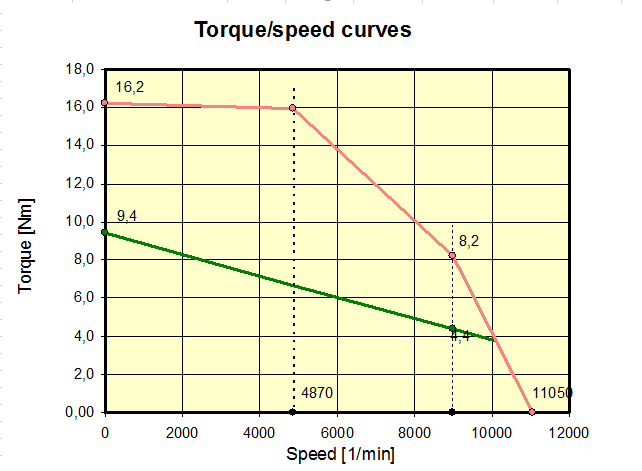
\includegraphics[width=\textwidth]{./img/MOTOR2-torque.png}
	\caption{Front motor characteristics.}
	\label{fig:torque2}
\end{figure}


\subsubsection{Wiring, cables, current calculations, connectors}
We use Raychem TR 16-10-0 and TR 16-6-0. There are leadthrough used for cables in motors and connectors Souriau „8STA 0 18 18” are used in Motor controllers.

\subsubsection{Position in car}
Front motors are situated directly in the front uprights.

\begin{figure}[H]
	\centering
	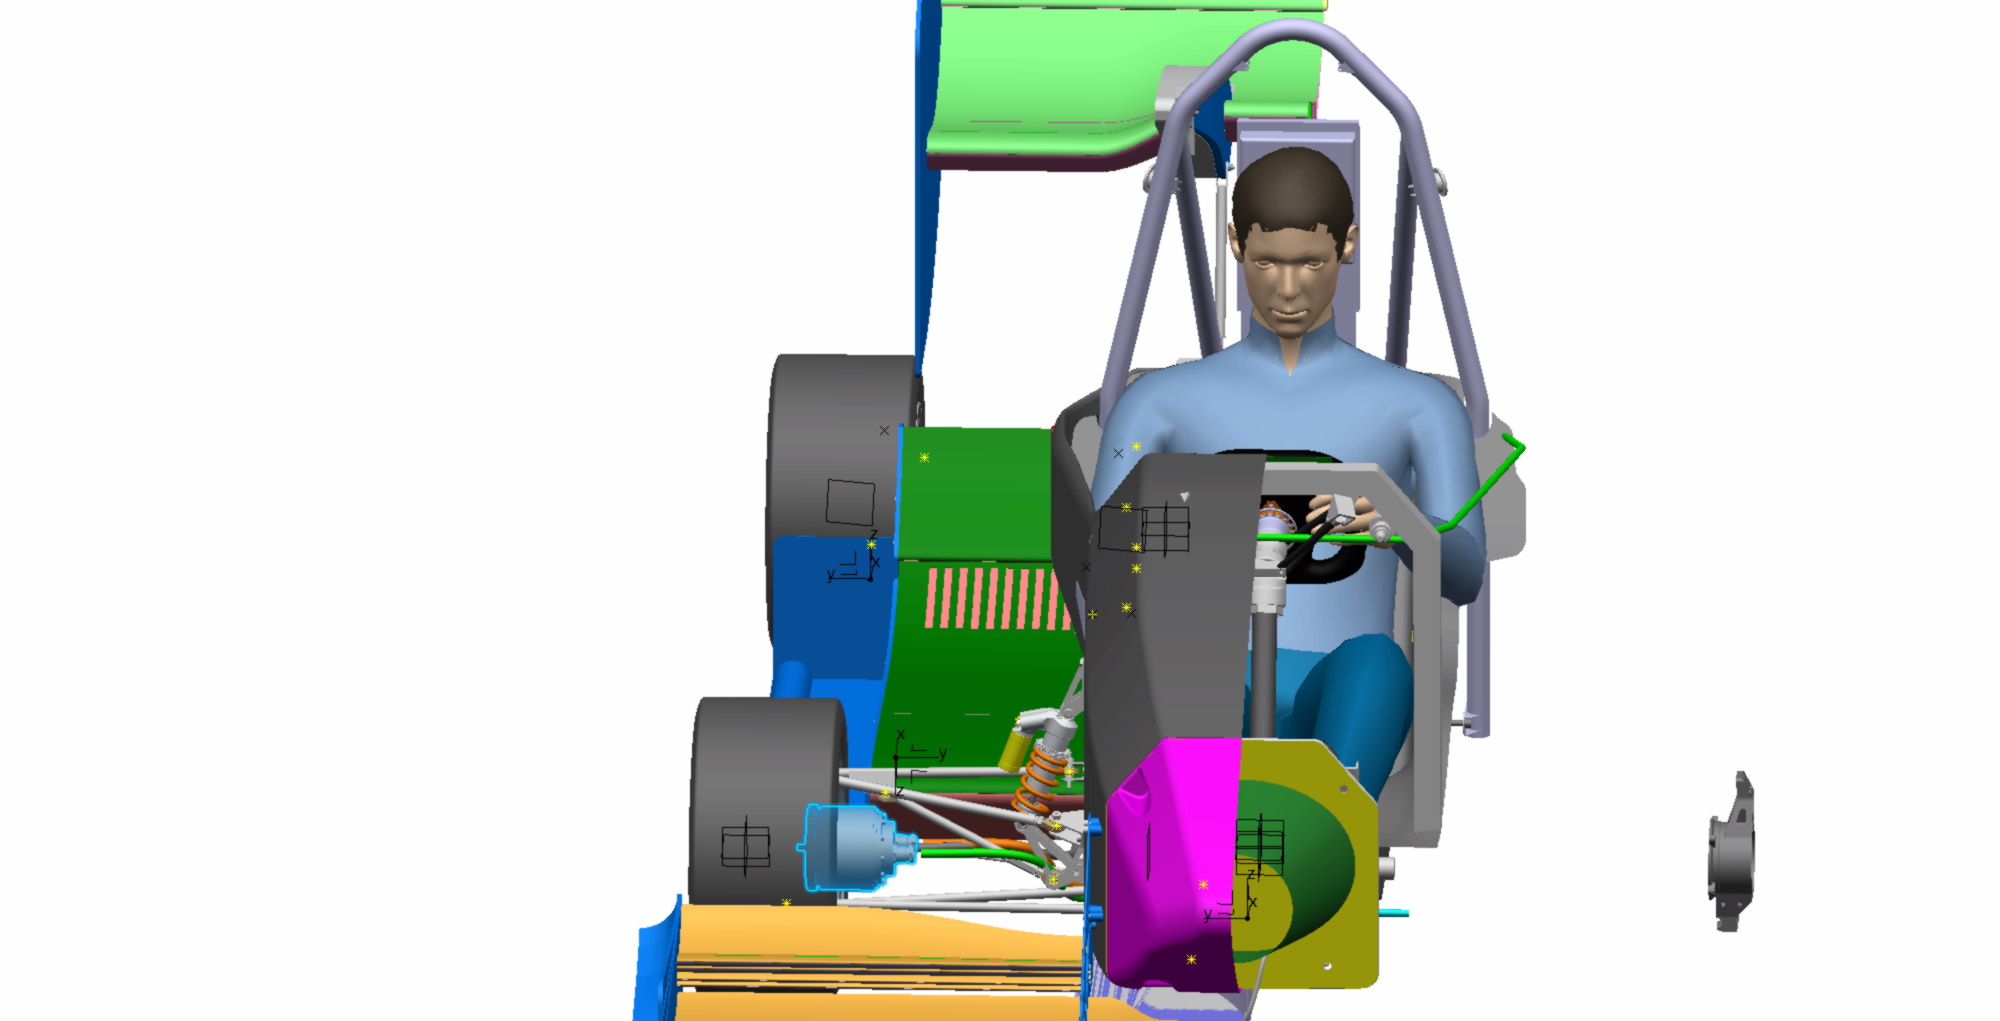
\includegraphics[width=\textwidth]{./img/Motor-front-position.jpg}
	\caption{Front motor position.}
	\label{fig:Motor-front-position}
\end{figure}




\newpage
\section{Torque Encoder}\label{sec:TorqueEncoder}
%Responsible: Bacha
%ECUP
\subsection{Description/additional circuitry}
Car is using two torque encoders for accelerator pedal. Encoders are linear potentiometers. Sensors are powered and measured by ECU-P (electrical control unit - pedals). They output analog voltage signal equal to accelerator pedal position. Both output signals goes through \label{fig:ecup_analog_input} and low pass filters. Then they are fed to ADC (analog to digital converter) and analyzed by MCU (microcontroller unit) for validity and plausability. Information about position and errors is send though CAN.

\begin{table}[H]
	\centering
	\caption{Torque encoder data}
	\begin{tabularx}{\textwidth}{|X|X|}
		\hline
		Torque encoder manufacturer: & TE connectivity  \\[\TableSize]\hline
		Torque encoder type: & MLP-50  \\[\TableSize]\hline
		Torque encoder principle: & linear potentiometer  \\[\TableSize]\hline
		Total number of Torque Encoder Sensors: & 2  \\[\TableSize]\hline
		Supply voltage: & +5V  \\[\TableSize]\hline
		Maximum supply current: & 1mA  \\[\TableSize]\hline
		Operating temperature: & -30degC to -150degC  \\[\TableSize]\hline
		Used output: & DC voltage 0V to 5V\\[\TableSize]\hline
	\end{tabularx}%
	\label{tab:encoder-general}%
\end{table}%

\subsection{Torque Encoder Plausability Check}
Torque encoder implausability, short circuit and open circuit checks are done by MCU. Sensors are powered from +5V. Used travel of sensors does not contain end positions. Converted analog signal ranges are normalized according to calibration.
If any following sensor error is detected, motor controllers are shut down and message is send through CAN to other units.

\paragraph{Electrical check} 
Using only part of whole range of sensor excluding end positions allows detection of signal short to Ground or voltages higher or equal to sensor's power voltage.

Analog input circuitry of ECUP is shown in \ref{fig:ecup_analog_input}. In normal conditions, signal from sensor (RAW) goes through R2, then is clamped by D1 and continues through R1 and C1 to filters and other circuits of ECUP (AIN). TEST signal is held \textit{low} but due to high resistance of R3 has minimal impact on input signal.

When ADC measures 0V or value close to 0V, TEST signal logic level is switched \textit{high} to charge C1 through R3. After short while, logic level of TEST signal is read back. If \textit{high} logic level is read, sensor input is evaluated as \textit{open circuit}, otherwise it is \textit{short circuit} to GND. If measured value is close to power voltage of sensor or above measurable range, it is evaluated as \textit{short circuit} to power voltage or higher.

\paragraph{Implausability}
Position values difference is calculated and compared with maximal allowed error threshold (10\%).

\begin{figure}[H]
\begin{center}
	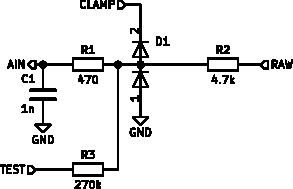
\includegraphics[width=0.5\textwidth]{./img/ECUP_AIN.pdf}
	\caption{ECU-P analog input circuit}
	\label{fig:ecup_analog_input}
\end{center}
\end{figure}



\subsection{Wiring}
\ref{fig:ecup_wiring} is diagram of sensor wiring.

\begin{figure}[H]
\begin{center}
	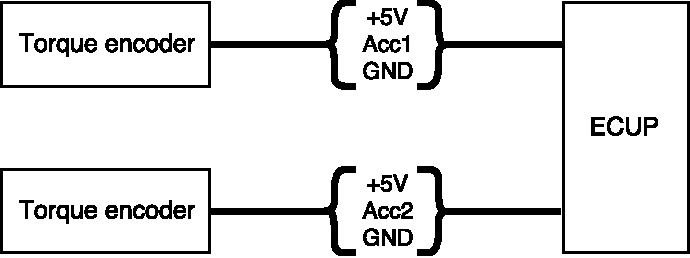
\includegraphics[width=0.5\textwidth]{./img/ECUP_wiring.pdf}
	\caption{ECU-P sensor wiring}
	\label{fig:ecup_wiring}
\end{center}
\end{figure}

\subsection{Position in car/mechanical fastening/mechanical connection}
In \ref{fig:torque_encoder_position} is shown position of two torque encoder sensors (piston shape objects).

\begin{figure}[H]
\begin{center}
	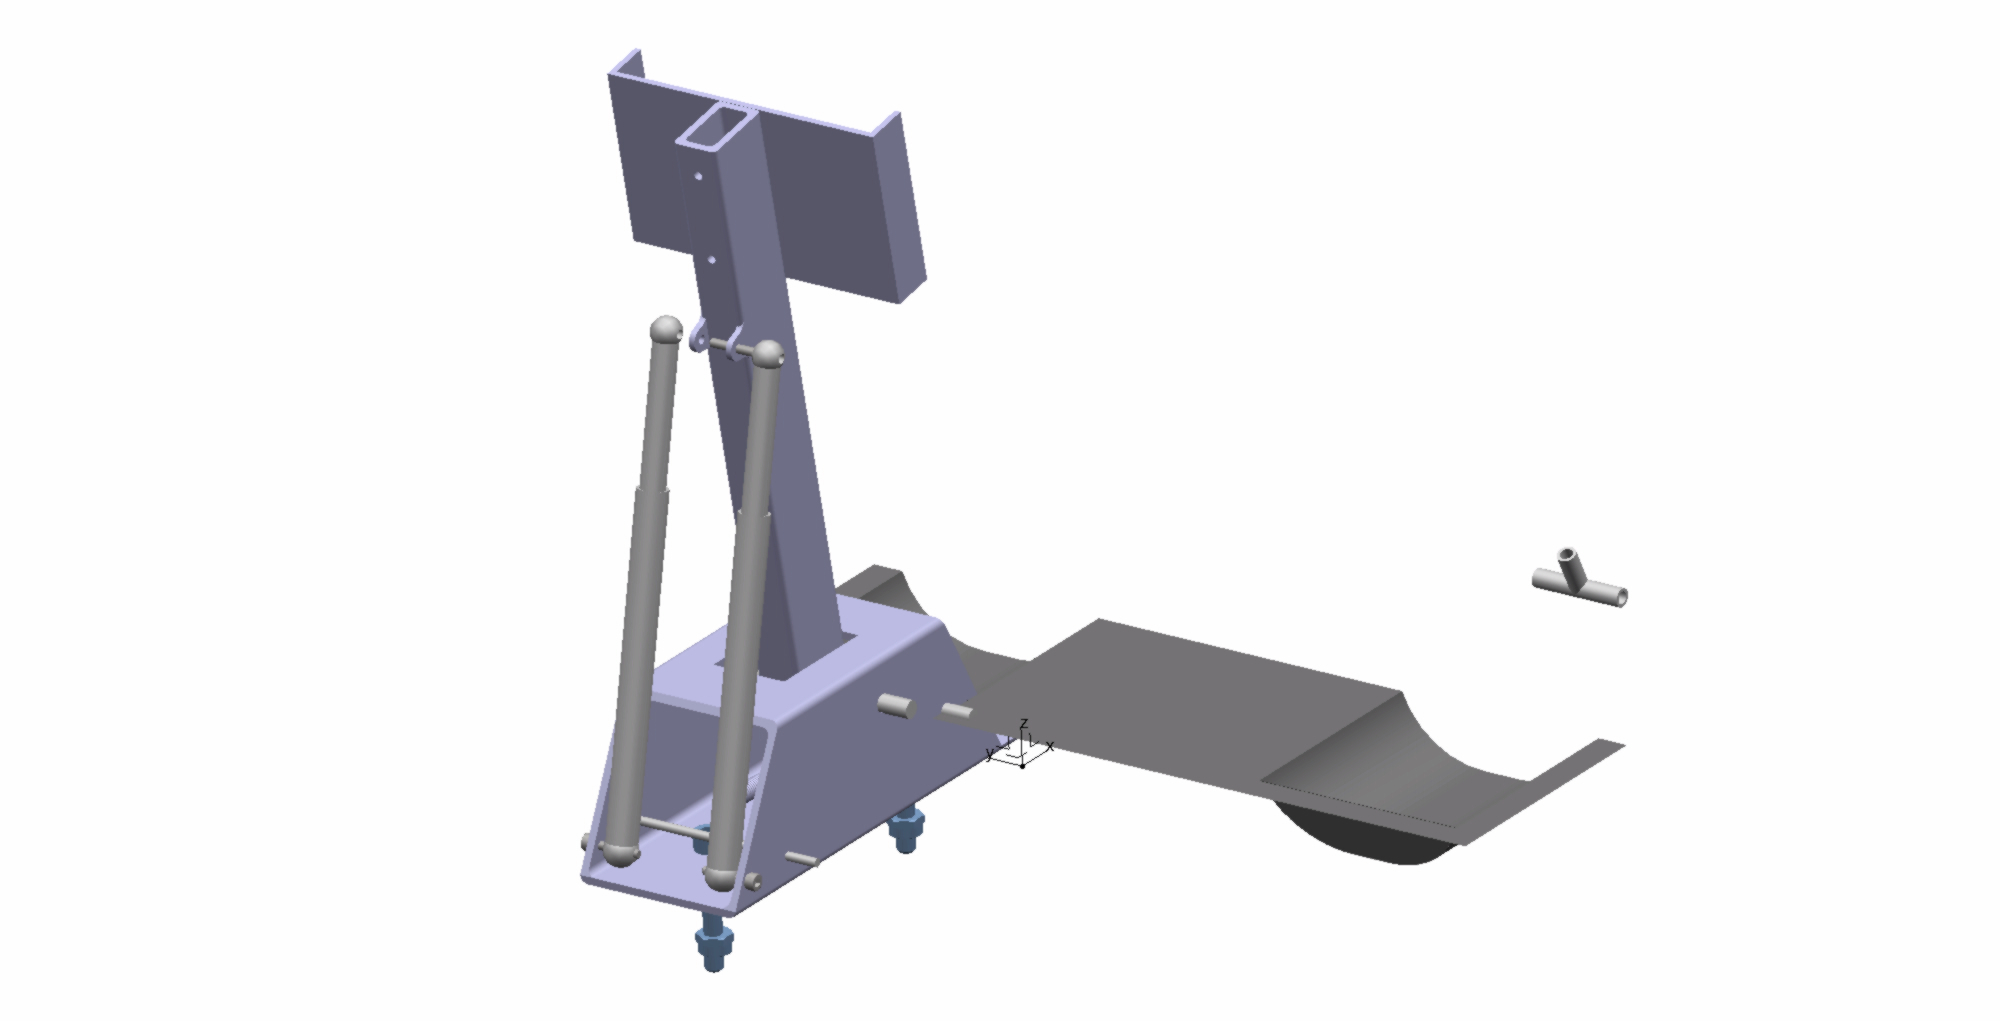
\includegraphics[width=0.8\textwidth]{./img/ACC-pedal-pos.jpg}
	\caption{Torque encoder position}
	\label{fig:torque_encoder_position}
\end{center}
\end{figure}



%\begin{figure}[H]
%\begin{center}
%	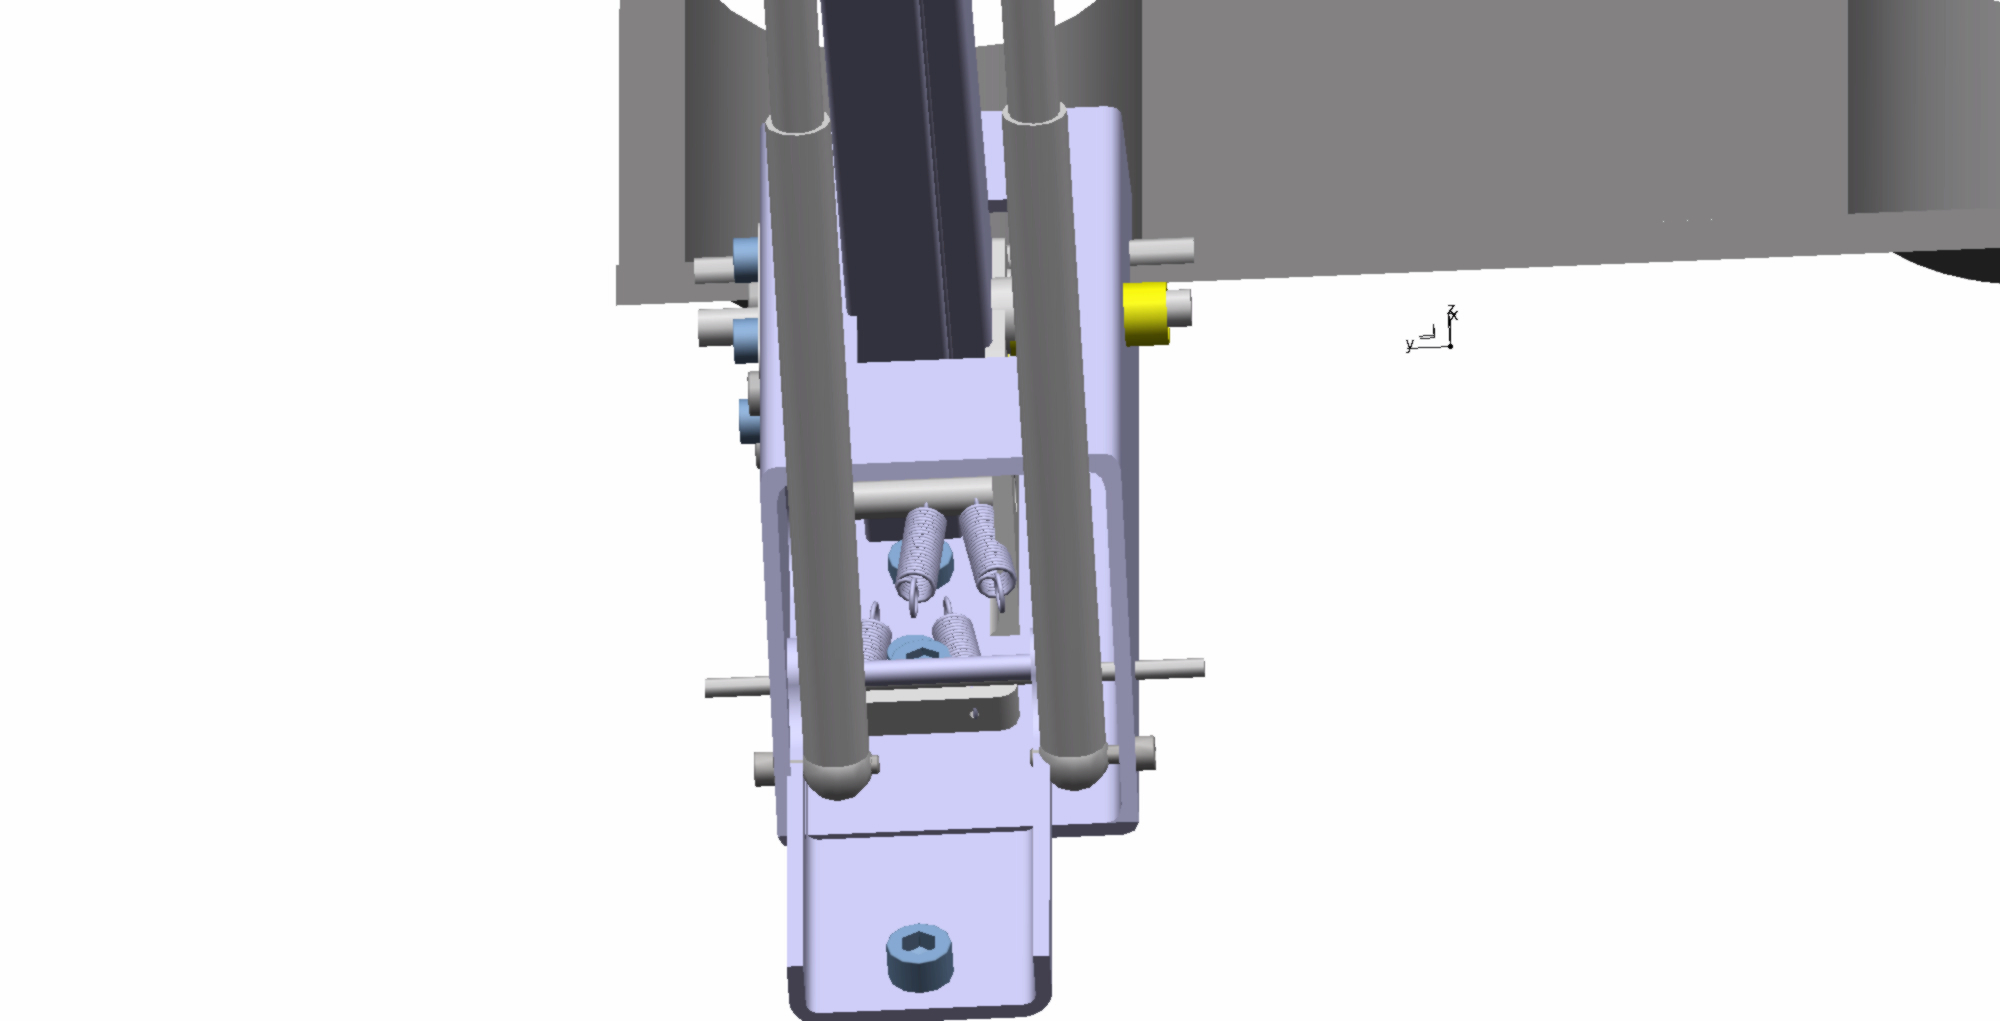
\includegraphics[width=0.8\textwidth]{./img/ACC-pedal-pos2.jpg}
%	\caption{Torque encoder position}
%	\label{fig:torque_encoder_position_alt}
%\end{center}
%\end{figure}




\newpage
\section{Brake Encoder}\label{sec:BrakeEncoder}%added
%Responsible: Bacha
%ECUP
\subsection{Description/additional circuitry}
Car is using two pressure sensors as encoders for brake pedal. Each one is for separate brake system. Sensors are powered and measured by ECU-P, same unit as \label{sec:TorqueEncoder}. Pressure sensors output analog voltage signal equal to brake system pressure. 

%\def\tabularxcolumn#1{m{#1}}

\begin{table}[H]
	\centering
	\caption{Brake encoder data}
	\begin{tabularx}{\textwidth}{|X|X|}
		\hline
		Torque encoder manufacturer: &  Keller \\[\TableSize]\hline
		Torque encoder type: & PA-21 Y \\[\TableSize]\hline
		Torque encoder principle: & pressure sensor \\[\TableSize]\hline
		Total number of Torque Encoder Sensors: & 2 \\[\TableSize]\hline
		Supply voltage: & +24V \\[\TableSize]\hline
		Maximum supply current: &  4mA  \\[\TableSize]\hline
		Operating temperature: & -40degC to 100degC \\[\TableSize]\hline
		Used output: & DC voltage 0,5V to 4,5 V \\[\TableSize]\hline
	\end{tabularx}%
	\label{tab:brake-general}%
\end{table}%

\subsection{Brake Encoder Plausability Check}
Implausability is not checked, because eForce does not use brake pedal information to control motor controllers.

%
%\subsection{Wiring}
%Describe the wiring, show schematics, show data regarding the cables and connectors used.
%
%\subsubsection{Position in car/mechanical fastening/mechanical connection}
%Provide CAD-renderings showing all relevant parts and discuss the mechanical connection of the sensors to the pedal assembly. Mark the parts in the rendering, if necessary.






\newpage
\section{Additional LV-parts interfering with tractive system}\label{sec:AdditionalLV}
\subsection{VDCU(Vehicle Dynamics Control Unit)}
VDCU is a vehicle dynamics control unit. It manipulates torque request from driver pedal to calculate final torque for all 4 motors. The calculated torque never exceed driver request as driver request is processed as torque limitation Traction control can only decrease the total amount of requested torque.

\subsubsection{Description}
Board uses only LV and 2x CAN bus.\\
HW :\\
-Texas Instruments C2000 Delfino F28377 MCU\\
-5V can transceiver TJA1049\\

\noindent SW:\\
Board is programmed using simulink embedded coder. Advantage is that we can use our developed code for IPG Carmaker simulation (MIL) directly into our formula. VDCU uses pedal position, inertial measurement, steering wheel sensor, wheel speed sensor and motor encoders to manipulate the torque. Measurements are fed into our yaw rate control system. Output is a torque vector fed to torque vectoring algorithm that calculates the torque distribution for all wheels The resultant torque for individual wheels is lowered by traction control algorithm if needed and fed to motors.

\begin{figure}[H]
	\centering
	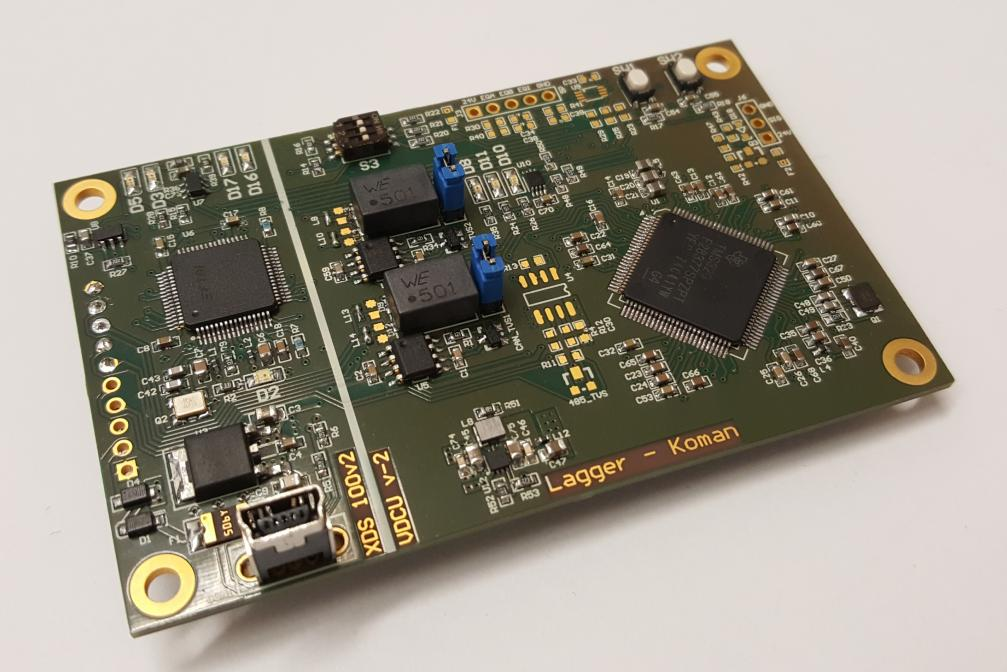
\includegraphics[width=\textwidth]{./img/VDCU-pcb.jpg}
	\caption{PCB of VDCU.}
	\label{fig:VDCU-pcb}
\end{figure}

\subsubsection{Wiring, cables}
Module is connected using headers to ECUB.

\subsubsection{Position in car}
Inside ECUB box.

\subsection{LV part 2}
Describe those parts here which interfere or influence the tractive system, for example a controlling unit that measures wheel speeds and steering angle and calculates a target torque for each motor or a DC/DC-Converter providing power for the LV-system from the HV-system, etc.

\subsubsection{Description}
Describe the parts used and their circuitry, and provide main operation parameters, use tables or figures, etc.

\subsubsection{Wiring, cables}
Describe the wiring, show schematics, etc.

\subsubsection{Position in car}
Provide CAD-renderings showing the relevant parts. Mark the parts in the rendering, if necessary.

\newpage
\section{Overall Grounding Concept}\label{sec:GroundingConcept}
%Zalaminovat, kopie
\subsection{Description of the Grounding Concept}
We are using net of thin wires from grounding point laminated into composite.
\subsection{Grounding Measurements}
For measuring we are using 4 point method with current power supply to ensure 5 Ohms. In carbon fiber we have copper wires.


\newpage
\section{Firewall}\label{sec:Firewall}
%Responsible: hotov
\subsection{Description/materials}
%Describe the concept, layer structure and the materials used for the firewall. Show how the low resistance Control System ground connection is achieved.

We are using standard concept of firewall as described in the rules (T4.5.4). So the firewall is made from 2 layers. The first one is 0,5 mm thick aluminum sheet and the second one is 0,8 mm thick glass fiber/polyester plastic sheet with UL 94-V0 certificate (type: UPM 203 / UPM 71/S included in appendix). These are glued together and bended to the shape of final firewall. Aluminum sheet is oriented to the dangerous side and glass fiber to the driver side.
\subsubsection{Position in car}
%Provide CAD-renderings showing all relevant parts. Mark the parts in the rendering, if necessary.

Firewalls are located behind the seat and above the front motor controller (under drivers knees). These firewalls are connected with "firewall tunnel" where are located the high voltage cables.

\begin{figure}[H]
	\centering
	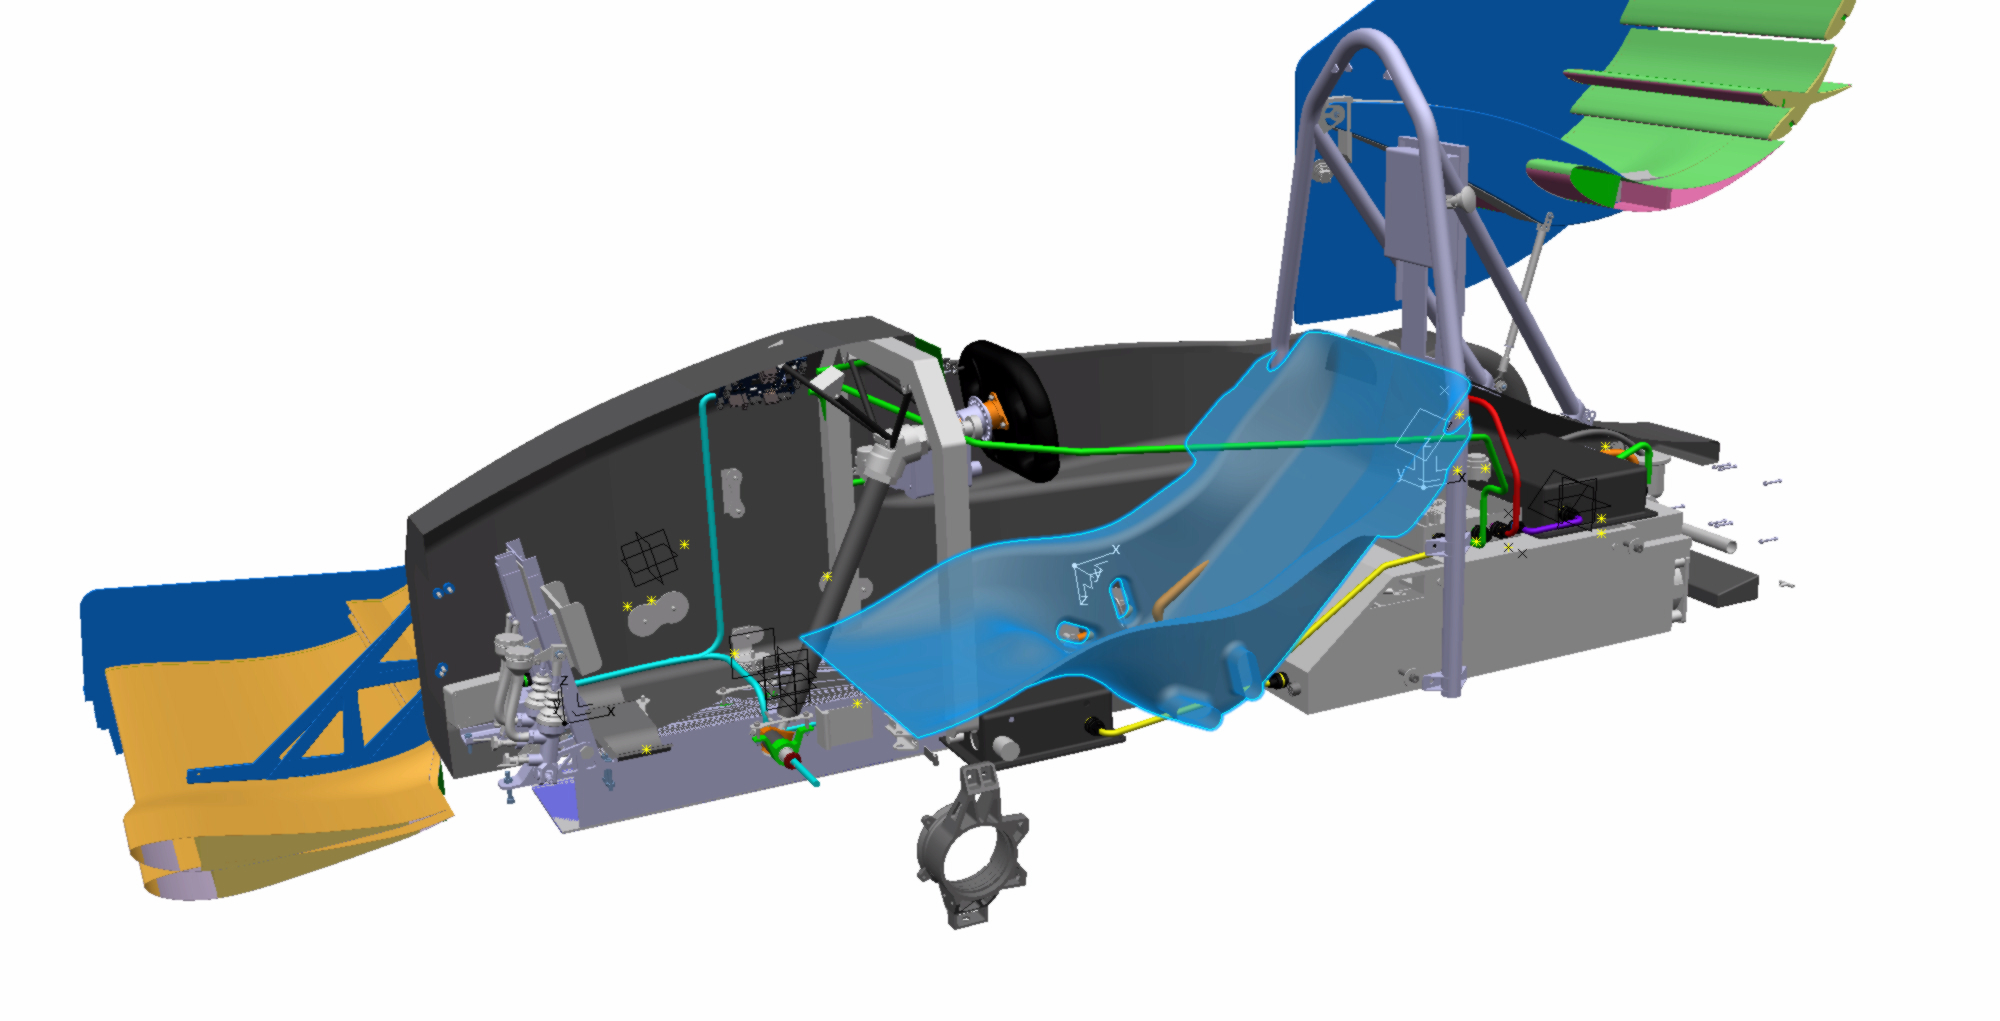
\includegraphics[width=\textwidth]{./img/Firewall-position.jpg}
	\caption{Firewall position.}
	\label{fig:Firewall-position}
\end{figure}

%------Appendix------
\appendix
%\setcounter{figure}{0} 
\renewcommand{\figurename}{Appendix}

\section{Appendix}\label{sec:Appendix}

\subsection{HV Disconnect (HVD)}

\begin{figure}[H]
	\centering
	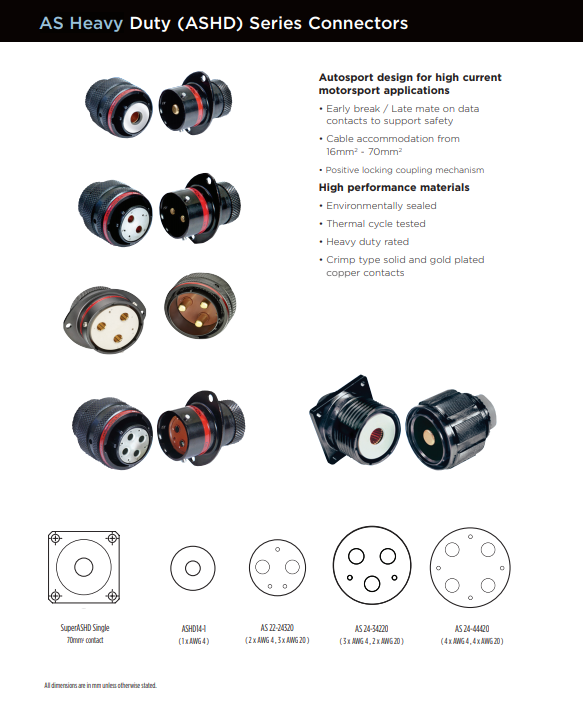
\includegraphics[width=\textwidth]{./img/app-HVD.png}
	\caption{HVD interlock datasheet.}
	\label{app:HVD}
\end{figure}

Full datasheet \url{http://www.te.com/commerce/DocumentDelivery/DDEController?Action=srchrtrv&DocNm=1-1773721-8_as_interconnection&DocType=DS&DocLang=EN}

\subsection{Motor controller}

Datasheet of NME1215SC, refered from \ref{sec:MotorController}.
\begin{figure}[H]
	\centering
	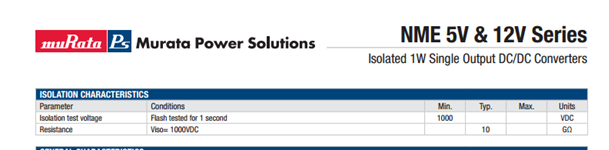
\includegraphics[width=\textwidth]{./img/NME1215SC.png}
	\caption{NME1215SC isolation.}
	\label{app:NME1215SC}
\end{figure}
Full datasheet to be found at \url{http://power.murata.com/data/power/ncl/kdc_nme.pdf}

\begin{figure}[H]
	\centering
	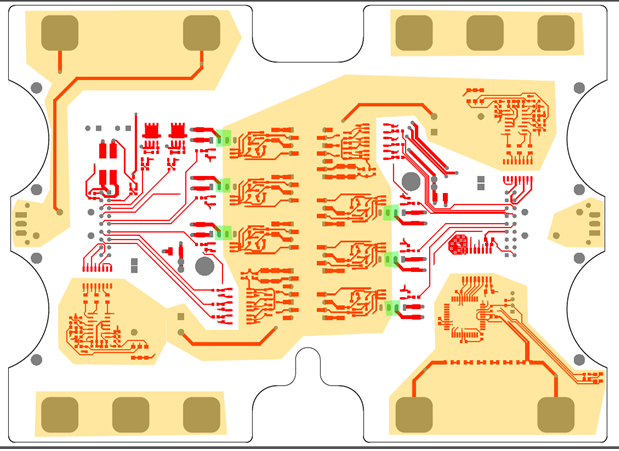
\includegraphics[width=.7\textwidth]{./img/mc-top.png}
	\caption{Motor controller TOP.}
	\label{app:mc-top}
\end{figure}

\begin{figure}[H]
	\centering
	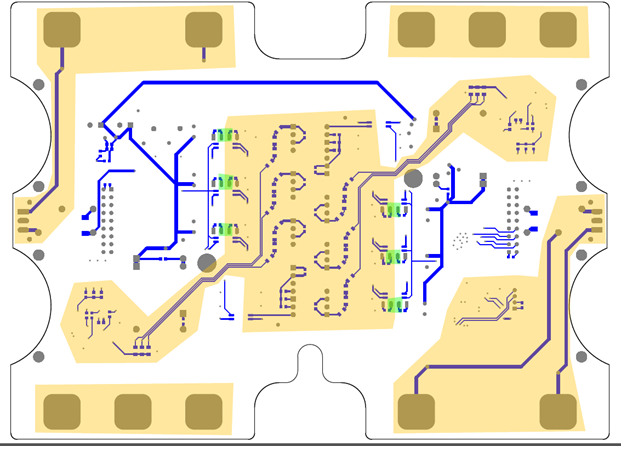
\includegraphics[width=.7\textwidth]{./img/mc-bot.png}
	\caption{Motor controller BOTTOM.}
	\label{app:mc-bot}
\end{figure}

\subsection{Motor}

\begin{figure}[H]
	\centering
	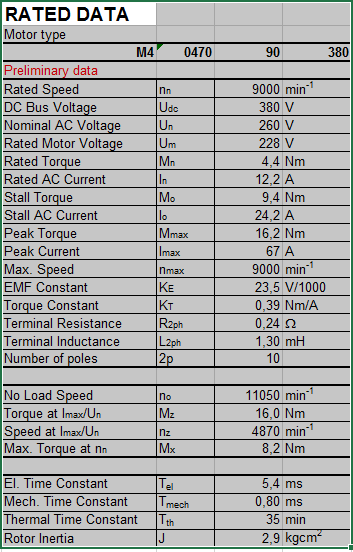
\includegraphics[width=0.3\textwidth]{./img/app-mf.png}
	\caption{Datasheet motor front.}
	\label{app:mf}
\end{figure}

\begin{figure}[H]
	\centering
	\includegraphics[width=.3\textwidth]{./img/app-mr.png}
	\caption{Motor controller BOTTOM.}
	\label{app:mr}
\end{figure}

\subsection{Overall Grounding Concept}

\subsection{Firewall}

\end{document}